\documentclass{article}

\usepackage{neurips_2026}

\usepackage[utf8]{inputenc}
\usepackage[T2A,T1]{fontenc}
\usepackage[english,russian]{babel}
\usepackage{tempora} % Times-подобный шрифт с кириллицей (T2A); заменяет ptm из neurips_2026.sty
\usepackage{hyperref}
\usepackage{url}
\usepackage{booktabs}
\usepackage{amsfonts}
\usepackage{amsmath}
\usepackage{nicefrac}
\usepackage{microtype}
\usepackage{xcolor}
\usepackage{graphicx}
\usepackage{array}
\usepackage{enumitem}
\usepackage{placeins}
\usepackage{tikz}
\usetikzlibrary{arrows.meta,positioning}

\newcommand{\method}[1]{\texttt{#1}}

\title{Q/R/M/C: измерительный фреймворк постадийной декомпозиции для навигации на основе памяти}

%\author{%
%  Anonymous Authors \\
%  Anonymous Institution \\
%  Anonymous Address \\
%  \texttt{anonymous@anonymous.edu} \\
%}

\begin{document}

\maketitle

\begin{abstract}
\textbf{Постановка.} Метрики, учитывающие только успех, схлопывают качественно различные отказы навигации на основе памяти в один скаляр, скрывая, \emph{какая стадия} конвейера извлечения (retrieval) за них ответственна. Данная статья вносит вклад в виде \emph{протокола оценивания} (evaluation protocol): постадийной декомпозиции Q/R/M/C (формирование запроса --- \textbf{Q}uery, удовлетворение извлечения --- \textbf{R}etrieval, материализация цели --- \textbf{M}aterialization, завершение после извлечения --- \textbf{C}ompletion), операционализированной так, что четыре условные частоты вычислимы непосредственно из стандартных логов траекторий (Определение~1). Арифметика --- это цепное правило, и это сделано намеренно: как декомпозиция accuracy на precision и recall не добавила математики, но изменила то, что поле смогло \emph{увидеть}, так и здесь ценность --- в идентифицируемости из логов и в том, что декомпозиция вскрывает, а не в теореме.
\textbf{Одноагентные измерения.} На 10-сидовом бенчмарке MiniGrid (FourRooms, LavaGapS7) и проверке переносимости на BabyAI фреймворк локализует бутылочные горлышки: восстановление после опасности ограничено извлечением (оракульное извлечение поднимает успех $0.39\to0.60$), возврат в целевой регион ограничен нижележащими стадиями. Инспекция логов уточняет атрибуцию: ранжирование кандидатов почти оптимально ($96.9\%$), тогда как генерация кандидатов отказывает в 91\% точек принятия решений --- это предел накопления памяти, а не ранжирования.
\textbf{Многоагентные измерения.} На многоагентном свипе из 35{,}640 прогонов по четырём коммуникационным архитектурам (независимая, общая шина, центральный агрегатор, широковещательная рассылка между пирами при восьми каденциях $K{\in}\{1,2,4,8,16,32,48,64\}$, 40 сидов) смещение бутылочного горлышка (bottleneck shift) между звеньями M и C проявляется напрямую как отрицательная внутрикаденционная корреляция с пиком при $K{=}4$ (Пирсон $-0.61$); среднее время до успеха имеет внутренний минимум при $K{=}8$ (устойчивый по положению, но мелкий по запасу --- не отличим от соседних быстрых каденций). Оба знака наклонов (Эмпирическое утверждение~1) подтверждаются как умеренные, кластерно-робастные размеры эффекта (Спирмен $-0.53$ и $+0.43$ от $K$, 95\%-е ДИ $[-0.59,-0.47]$ и $[+0.37,+0.50]$ по 81 конфигурационной ячейке; Приложение~\ref{app:effect-sizes}). Не-утверждения (в частности, об условном произведении $\Phi$) собраны в одном месте (\S1, «Границы применимости и не-утверждения»).
\textbf{Диагностическое применение.} Те же четыре частоты также показывают, почему обученные политики с неявной коммуникацией могут быть конкурентоспособны по успеху, при этом схлопывая наблюдаемость Q/R/M/C: их коммуникационные векторы никогда не бывают информативно пустыми, и у них нет явного интерфейса фиксации цели. На двух локальных LLM-агентах (qwen3:4b, llama3.1 на TextNav) тот же логгер локализует отказ, ограниченный завершением: при жёстком бюджете шагов оба агента формируют запрос, извлекают и фиксируют цель ($Q^\star{=}R^\star{=}M^\star{=}1$), но ни один не завершает ($C^\star{=}0$), так что в остальном непрозрачный провал успеха разрешается в конкретную отказывающую стадию, а не в число в лидерборде. Таким образом, вклад --- это измерительный протокол, делающий отказы памяти сопоставимыми между символьными, обученными, LLM-, одноагентными и многоагентными системами.
\textbf{Границы применимости.} Основные эксперименты проведены в grid-world-субстратах (MiniGrid, BabyAI, собственная сетка $12{\times}10$). Вклад --- диагностический фреймворк и его валидация; предварительная проверка в непрерывном пространстве состояний на VMAS воспроизводит оба знака наклонов направленно (Приложение~\ref{app:vmas}), а полная валидация в непрерывных/3D-средах с кластерно-робастными ДИ (Habitat, ProcTHOR) --- предмет будущей работы.
\end{abstract}

\section{Введение}

\begin{figure}[t]
  \centering
  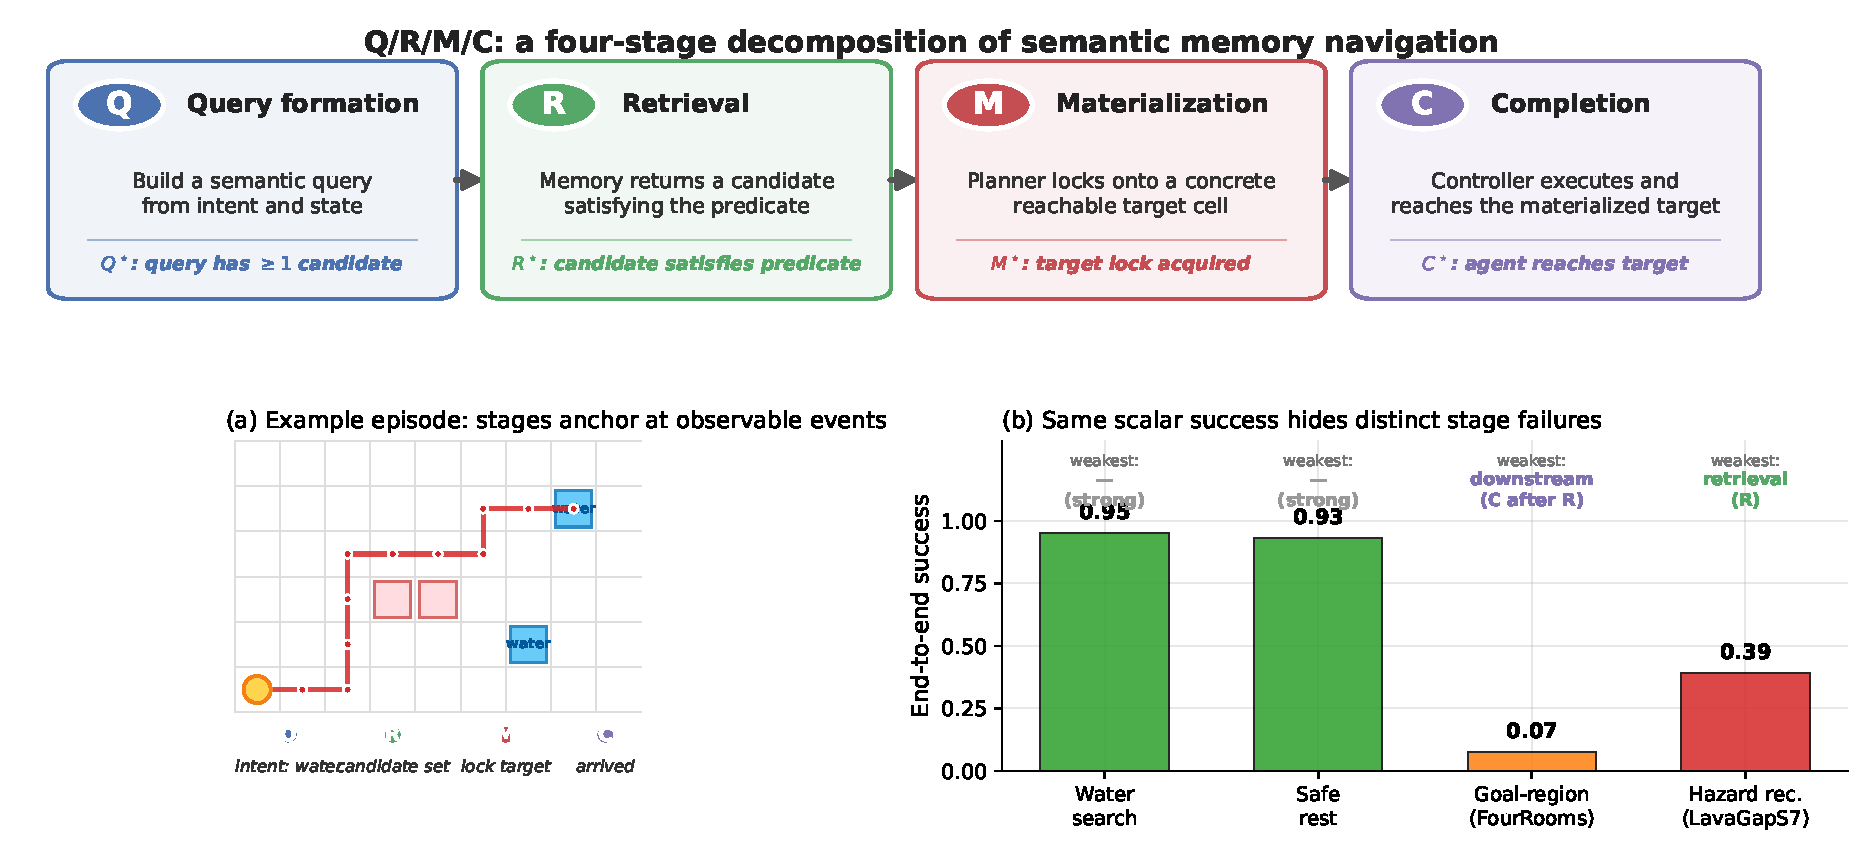
\includegraphics[width=\linewidth]{figures/fig_hero_qrmc.pdf}
  \caption{Q/R/M/C раскладывает один эпизод семантической навигации на четыре
  наблюдаемые стадии. \textbf{Сверху:} четыре стадии и их определения на уровне
  событий. \textbf{(a)}~Успешный эпизод поиска воды закрепляется
  на одном событии на стадию, порождая логируемые «звёздные» события
  $Q^\star, R^\star, M^\star, C^\star$. \textbf{(b)}~Одна и та же скалярная
  сводка «сквозного успеха» маскирует качественно различные отказы
  на четырёх одноагентных семействах задач: вода и отдых сильны;
  возврат в целевой регион (FourRooms) ограничен нижележащими стадиями; восстановление
  после опасности (LavaGapS7) ограничено извлечением (оракульные интервенции, \S\ref{sec:oracle}).}
  \label{fig:hero}
\end{figure}

Классические навигационные бенчмарки часто предполагают, что агенту дана
явная координата пункта назначения или плотная награда за задачу. Многие практические
навигационные задачи устроены иначе: агент должен достичь места определённого
\emph{типа} --- безопасной зоны отдыха, водоподобного ресурса,
выхода для восстановления после опасности или региона, ассоциированного с целью, ---
заданного семантическим паттерном, а не фиксированной путевой точкой $(x, y)$. Следовательно, место
должно быть \emph{запомнено и извлечено по смыслу}. Эта
постановка открывает методологический вопрос: можем ли мы измерить, \emph{где}
ломается семантическая навигация на основе памяти, а не только \emph{ломается ли}
она?

Мы отвечаем на этот вопрос четырёхстадийным диагностическим фреймворком,
применимым как к одиночным агентам, так и к многоагентным коллективам.
Декомпозиция --- Q/R/M/C: формирование запроса (\textbf{Q}uery formation), удовлетворение
извлечения (\textbf{R}etrieval satisfaction), материализация цели (target \textbf{M}aterialization) и завершение
после извлечения (\textbf{C}ompletion after retrieval). Декомпозиция факторизует поэпизодное завершение семантического
пути, и при условном постадийно-марковском свойстве её факторы
оцениваемы из логов траекторий (Определение~1).
Остальная часть статьи развивает единый аргумент в трёх частях.

\textbf{Одиночный агент.} Постадийная атрибуция нетривиальна.
Метрики только успеха схлопывают качественно различные отказы в
один скаляр. В 10-сидовом бенчмарке MiniGrid задачи воды и отдыха
сильны сквозным образом (успех 0.95, 0.93), но возврат в целевой регион и
восстановление после опасности существенно труднее, причём по \emph{разным
причинам}. Оракульные постадийные интервенции показывают, что восстановление после опасности
ограничено извлечением (оракульное извлечение поднимает успех $0.39 \to 0.60$),
тогда как возврат в целевой регион ограничен нижележащими стадиями (оракульное извлечение
спасает завершение семантического пути, не меняя сквозного успеха).
Инспекция собственных логов фреймворка затем заостряет атрибуцию:
бутылочное горлышко извлечения --- не \emph{ранжирование} кандидатов (точность
$96.9\%$, когда кандидаты существуют), а их \emph{генерация}:
память не содержит подходящих символов в 91\% точек принятия решений.
Одноагентное бутылочное горлышко --- предел \emph{накопления памяти}:
свидетельства наблюдаются, но так и не консолидируются в структуру, доступную запросам.

\textbf{Много агентов.} Консолидация обретает темп.
Когда $N$ агентов разделяют память через широковещательный протокол с каденцией (cadence)
$K$, факторизация расширяется укрупнёнными множествами обусловливания
(Определение~2), и $K$ становится структурной осью: механически это
ручка, регулирующая, \emph{насколько быстро приватные памяти консолидируются
в коллективную}. Утверждение на уровне наклонов
(Эмпирическое утверждение~1) предсказывает смещение бутылочного горлышка: с уменьшением $K$
$P(M^\star|R^\star)$ растёт (более свежая память пиров позволяет
надёжно коммититься), а $P(C^\star|M^\star)$ падает (пиры соревнуются за
одни и те же цели). Оба знака наклонов подтверждены на свипе из 35{,}640 прогонов
как умеренные, кластерно-робастные размеры эффекта (Приложение~\ref{app:effect-sizes}); сдвиг напрямую виден как отрицательная
внутрикаденционная корреляция между двумя звеньями, а результирующий
компромисс порождает внутренний оптимум среднего времени до успеха при
$K\!=\!8$: у консолидации есть нетривиальный оптимальный темп.

\textbf{Диагностический синтез.} Оба режима указывают на один и тот же
объект измерения. Одноагентный диагноз говорит, что консолидация
свидетельств в символы может быть связывающим ограничением; многоагентный
диагноз говорит, что темп и цена обмена
консолидированной памятью определяют оптимум. Q/R/M/C --- общий
инструмент: системы-кандидаты можно сравнивать по тому, как они сдвигают
$P(R^\star|Q^\star)$, $P(M^\star|R^\star)$ и
$P(C^\star|M^\star)$, даже когда их сквозные показатели успеха выглядят
похоже.

\begin{center}
\fbox{\parbox{0.94\linewidth}{
\textbf{Границы применимости и не-утверждения (консолидировано).} Все оговорки этой
статьи в одном месте; основной текст их больше не повторяет.
(i)~Аргумент состоятельности декомпозиции --- это цепное правило плюс
частотное оценивание --- математическая новизна не заявляется; вклад ---
дисциплина логирования и идентифицируемость
(Определения~1--2). (ii)~Эмпирическое утверждение~1 --- проверенное наблюдение
на уровне наклонов об условных частотах, а не теорема.
(iii)~Мы не делаем утверждений о форме условного произведения
$\Phi$; в наших данных оно монотонно по $K$, а внутренний оптимум
живёт на среднем времени до успеха (\S\ref{sec:multi-agent-results}).
(iv)~Основные субстраты --- grid worlds; VMAS --- направленная
проверка в непрерывном пространстве состояний, а LLM-исследования малы и контролируемы
(две локальные модели на TextNav; коллектив $N{=}3$; внешняя валидация
на трёх фреймворках при $n{=}8$ на ячейку, \S\ref{sec:external}). (v)~Идентичность мест в многоагентном случае предполагает
общую систему координат (\S\ref{sec:limitations}). Постадийная
операционализация проверяема на конкретных сводках и может быть
\emph{неверной} на других --- (iii) как раз такой случай, --- что и
отличает измерительный протокол от догадки, безразличной к стадиям.}}
\end{center}

\textbf{Почему такая рамка своевременна.} Воплощённые и целеобусловленные
агенты всё чаще извлекают места, объекты или инструменты по смыслу
\citep{andrychowicz2017hindsight,ghosh2021learning,savva2019habitat}.
Системы LLM-агентов опираются на явные слои памяти, но оцениваются в основном
сквозным образом \citep{wang2023voyager,shinn2023reflexion,packer2023memgpt}.
Многоагентное обучение с подкреплением также всё чаще вовлекает
коммуницирующие популяции \citep{lowe2017maddpg,foerster2018ctde}, однако
вопросу «какой агент должен знать что и когда?» недостаёт
единого диагностического словаря. Наш фреймворк его даёт.

\textbf{Вклады.} Это методологическая статья. Мы явно разделяем, что здесь бухгалтерия, что эмпирическое утверждение, а что инстанцированный артефакт.
\begin{enumerate}[leftmargin=20pt,itemsep=2pt,topsep=2pt]
\item \textbf{Измерительный протокол (один агент).} Декомпозиция Q/R/M/C операционализирована так, что условные частоты оцениваемы из логов траекторий (Определение~1); вклад --- \emph{дисциплина логирования}, делающая декомпозицию применимой к стандартным навигационным трассам (не-утверждения: см. бокс выше).

\item \textbf{Измерительный протокол (много агентов).} Расширение на $N$ коммуницирующих агентов с двумя каналами связывания (память $\mathcal{M}_{-i}^{(K)}$, занятость $\mathcal{O}_{-i}$) при протоколе широковещательной рассылки между пирами с каденцией $K$ (Определение~2).

\item \textbf{Эмпирическое утверждение~1 (смещение бутылочного горлышка).} На многоагентном свипе из 35{,}640 прогонов оба стилизованных условия на наклоны \textbf{(F)} и \textbf{(O)} подтверждены как умеренные, кластерно-робастные размеры эффекта (Спирмен $-0.53$ и $+0.43$ от $K$, 95\%-е ДИ, исключающие ноль, по 81 конфигурационной ячейке; Приложение~\ref{app:effect-sizes}; полный бенчмарк в \S\ref{sec:multi-agent-results}), с механизмом на уровне провенанса (provenance) (\S\ref{sec:multi-agent-results}).

\item \textbf{Система и бенчмарки.} Символьно-семантический стек памяти с четырьмя коммуникационными архитектурами (независимая, общая шина, центральный агрегатор, широковещательная рассылка peer-to-peer); одноагентный оракульный бенчмарк (10-сидовый MiniGrid, переносимость на BabyAI); многоагентный свип из 35{,}640 прогонов при $N\!\in\!\{3,5,8\}$ + масштабирование на 8{,}640 прогонов при $N\!=\!12$; свип переносимости из 100 прогонов на обёртке стандартного MiniGrid.

\item \textbf{Диагностическое сравнение архитектур.} Один и тот же контракт логирования отделяет символьные системы памяти от обученных политик с неявной коммуникацией: последние могут быть конкурентоспособны по успеху, схлопывая при этом постадийную наблюдаемость Q/R/M/C. Это результат оценивания, а не утверждение, что один класс архитектур должен всегда доминировать.

\item \textbf{Границы и честность.} Основные эксперименты --- в grid-world-субстратах. Мы рассматриваем это как выбор, характерный для методологической статьи, и заявляем его явно (\S\ref{sec:limitations}); включена предварительная проверка VMAS на непрерывном субстрате (Приложение~\ref{app:vmas}), а полная валидация в непрерывных/3D-средах (Habitat, ProcTHOR, MineDojo) --- будущая работа.
\end{enumerate}

\section{Декомпозиция Q/R/M/C}
\label{sec:framework}

\subsection{Постановка задачи и нотация}
\label{sec:notation}

Агент действует в частично наблюдаемой навигационной среде.
На каждом шаге он получает наблюдение $o_t$, поддерживает состояние памяти
$\mathcal{M}_t$ и формирует запрос $q_t$, кодирующий текущее
намерение задачи. Шаг извлечения возвращает из $\mathcal{M}_t$ множество мест-кандидатов,
соответствующих $q_t$; выбранный кандидат
материализуется в действенную цель; локальный контроллер исполняет
действия, пока цель не достигнута или эпизод не истёк по времени.
Цель --- не координата, а семантический паттерн, поэтому успех есть
функция семантического профиля выбранного кандидата, а не какой-либо
заранее заданной координаты.

Habitat, AI2-THOR и ProcTHOR сделали визуально богатое оценивание навигации
стандартом
\citep{savva2019habitat,kolve2017ai2thor,deitke2022procthor}. Мы
намеренно фокусируемся на средах класса MiniGrid, чтобы получить чистые и
воспроизводимые постадийные измерения, а BabyAI используем только как проверку
переносимости. Мы не претендуем здесь на решение проблемы памяти LLM-агентов; скорее, мы
утверждаем, что та же декомпозиция Q/R/M/C --- полезный шаблон для
оценивания решений агентов, опирающихся на память, за пределами навигации.

Центральный эмпирический вопрос, таким образом, не просто в том, успешен ли агент,
а в том, \emph{какая стадия отказывает первой}, когда он неуспешен. Используются два
связанных измерительных слоя. \textbf{Операциональные частоты} считают,
на каждую попытку запроса, дал ли запрос непустое множество кандидатов,
удовлетворил ли выбранный кандидат семантическому предикату
и был ли он материализован в действенную цель;
\emph{завершение после извлечения} --- индикатор уровня эпизода.
\textbf{Вложенные события уровня эпизода}
$Q^\star \Rightarrow R^\star \Rightarrow M^\star \Rightarrow C^\star$
используются в факторизации ниже и аудируются в
\S\ref{sec:validation}. Полные операциональные определения даны в
Приложении~\ref{app:estimators}.

\textbf{Нотация.} Четыре стадии --- $Q$, $R$, $M$, $C$ со «звёздными» событиями уровня эпизода $Q^\star,R^\star,M^\star,C^\star\!\in\!\{0,1\}$, вложенными по построению. $P(\cdot)$ обозначает популяционную вероятность; $\hat{P}(\cdot)$ --- её эмпирико-частотную оценку. \textbf{Буква $M$ всегда обозначает стадию материализации; число целей в многоагентной среде записывается как $T$ (не $M$, ограничение $T{\le}N$, «дефицит» = $N{>}T$).} Прочие символы: $\mathcal{C}_K$ --- протокол широковещательной рассылки между пирами с каденцией $K$, $\mathcal{M}_{-i}^{(K)}$ --- снимки памяти пиров, $\mathcal{O}_{-i}$ --- занятость пиров, $\nu(\cdot)$ --- функционал свежести, $\Phi(K){=}P(M^\star|R^\star;K)\!\cdot\!P(C^\star|M^\star;K)$, $t_{\mathrm{succ}}$ --- среднее время до успеха. Полная таблица символов в Приложении~\ref{app:notation}.

\subsection{Одноагентная факторизация}
\label{sec:single-theory}

Пусть $Y$ обозначает общий успех эпизода, а
$Q^\star, R^\star, M^\star, C^\star$ --- вложенные события семантического пути
уровня эпизода. Фреймворк факторизует \emph{завершение семантического
пути}, а не сырой успех задачи:
\[
Q^\star \rightarrow R^\star \rightarrow M^\star \rightarrow C^\star.
\]
Для любого запроса $q$ и состояния памяти $\mathcal{M}$
\begin{align*}
P(C^\star = 1 \mid q, \mathcal{M})
&=
P(Q^\star = 1 \mid q, \mathcal{M})\;
P(R^\star = 1 \mid Q^\star = 1, q, \mathcal{M}) \\
&\quad \cdot
P(M^\star = 1 \mid R^\star = 1, q, \mathcal{M})\;
P(C^\star = 1 \mid M^\star = 1, q, \mathcal{M}).
\end{align*}
Общий успех задачи $Y$ может превышать $C^\star$, поскольку некоторые эпизоды
успешны без прохождения полного семантического пути извлечения.

\paragraph{Предположение 1 (условное постадийно-марковское свойство).}
При условии успешности текущей стадии вероятность
следующей стадии зависит только от текущей успешной стадии,
текущего запроса и текущего состояния памяти. Формально,
\[
P(R^\star \mid Q^\star, q, \mathcal{M}, \text{история}) = P(R^\star \mid Q^\star, q, \mathcal{M}),
\]
и аналогично для $M^\star$ и $C^\star$.

\paragraph{Предположение 2 (положительность).}
Каждое используемое выше событие обусловливания имеет ненулевую вероятность на
носителе бенчмарка.

\paragraph{Определение 1 (одноагентная оцениваемость стадий).}
При Предположениях 1--2 четыре условные частоты в факторизации выше являются корректно определёнными популяционными величинами, а эмпирико-частотные оценки --- их состоятельными оценками; их произведение сходится к завершению семантического пути. Аргумент элементарен --- факторизация по цепному правилу плюс состоятельность частотных оценок на бернуллиевских событиях --- и ценность его формулирования операциональна, а не математична: он фиксирует \emph{дисциплину логирования} (какие события, при каком обусловливании), при которой декомпозиция читаема из стандартных логов траекторий, и является контрактом, на соответствие которому аудируется каждый эксперимент этой статьи (\S\ref{sec:validation}). Полная формулировка и элементарный аргумент в Приложении~\ref{app:proofs}.

\paragraph{Когда Предположение~1 может нарушаться.}
Предположение~1 здесь выполняется жёстко, потому что $q$ и $\mathcal{M}$
явно логируются при каждом стадийном событии. Остаются два практически значимых
нарушения: адаптивные внутриэпизодные переписывания запроса, не всплывающие в
логгер, и скрытые межстадийные обновления памяти. В этих случаях
факторизацию следует читать как проекцию на наблюдаемые
трассы, а не как полное утверждение о структурной идентификации.
Приложение~\ref{app:assumption1-stress} количественно оценивает смещение оценки
при контролируемом нарушении такого рода: оно пренебрежимо при мягких
нелогируемых связываниях и однознаково (смещение вверх у
$P(C^\star|M^\star)$), что ограничивает уязвимость фреймворка при его
применении к обученным или LLM-агентам.

\paragraph{Механизменное прочтение.}
Та же декомпозиция допускает стадийно-структурированную механизменную
интерпретацию. Рисунок~\ref{fig:causal} трактует исходы стадий как
направленный ациклический граф. При такой интерпретации абляции включения/выключения
ассиста --- это нацеленные на механизм возмущения материализации и
пост-извлеченческого исполнения, а не недифференцированный анализ
чувствительности; в многоагентной постановке тот же граф реплицируется на
агента и связывается через каденционный протокол $\mathcal{C}_K$,
который действует на $\mathcal{M}_{-i}^{(K)}$ на ребре R$\to$M и на
$\mathcal{O}_{-i}$ на ребре M$\to$C --- ровно те два ребра, где
Эмпирическое утверждение~1 предскажет сдвиг наклонов.

\begin{figure}[t]
  \centering
  \begin{tikzpicture}[
    node distance=7mm and 7mm,
    box/.style={draw, rounded corners, align=center, minimum height=8mm, minimum width=15mm, fill=blue!8},
    arrow/.style={-{Latex[length=2.0mm]}, thick},
    assist/.style={draw, rounded corners, align=center, minimum height=7mm, minimum width=18mm, fill=orange!15}
  ]
    \node[box] (q) {$Q$};
    \node[box, right=of q] (r) {$R$};
    \node[box, right=of r] (m) {$M$};
    \node[box, right=of m] (c) {$C$};
    \node[box, right=of c] (s) {успех};
    \node[assist, above=of m] (a) {абляция\\ассиста};
    \draw[arrow] (q) -- (r);
    \draw[arrow] (r) -- (m);
    \draw[arrow] (m) -- (c);
    \draw[arrow] (c) -- (s);
    \draw[arrow] (a) -- (m);
    \draw[arrow] (a) -- (c);
  \end{tikzpicture}
  \caption{Стадийно-структурированная интерпретация фреймворка Q/R/M/C. Абляции включения/выключения ассиста нацелены на промежуточные механизмы; в многоагентном расширении каденционный протокол $\mathcal{C}_K$ действует на рёбра R$\to$M и M$\to$C.}
  \label{fig:causal}
\end{figure}

\paragraph{Связь с предшествующими работами.} Ближайшие направления: (i) фреймворки когнитивных и семантических карт \citep{tolman1948cognitive,okeefe1978hippocampus,kuipers2000spatial,gupta2017cognitive,savinov2018semi}, (ii) целеобусловленный RL и RL с репрезентациями преемника \citep{andrychowicz2017hindsight,ghosh2021learning,dayan1993improving,stachenfeld2017hippocampus,momennejad2017successor}, (iii) многоагентная коммуникация \citep{lowe2017maddpg,foerster2018ctde,sukhbaatar2016commnet,foerster2016learning} и gossip/консенсус \citep{boyd2006gossip,xiao2007distributed}, а также (iv) слои памяти LLM-агентов, оцениваемые сквозным образом \citep{wang2023voyager,shinn2023reflexion,packer2023memgpt}. Наш фреймворк ортогонален всем четырём: он \emph{диагностирует}, где в цепочке Q/R/M/C данная архитектура успешна или отказывает, и поднимает ось каденции с уровня сетевых протоколов до параметра когнитивной архитектуры (полное обсуждение в Приложении~\ref{app:related-work-extended}).

\subsection{Семантика событий, ограниченная рациональность и теоретико-порядковое прочтение}
\label{sec:event-semantics}

Четыре «звёздных» события закрепляются на конкретных логируемых триггерах. Мы формулируем триггеры один раз, поскольку каждое эмпирическое утверждение статьи --- это утверждение о них (формальные определения по режимам в Приложении~\ref{app:estimators}), и даём каждой стадии прочтение в терминах ресурса, который она ограничивает.

\begin{description}[leftmargin=10pt,topsep=2pt,itemsep=2pt]
\item[$Q^\star$ (намерение выпущено).] Планировщик выпускает семантическое намерение $q=(q^{\mathrm{req}},q^{\mathrm{pref}},q^{\mathrm{pen}})$: малые множества обязательных, предпочтительных и штрафных тегов. Событие уровня эпизода срабатывает при выпуске, поэтому оно насыщено всякий раз, когда задача семантична ($\hat P(Q^\star){=}1.00$ в Таблице~\ref{tab:consistency}); многоагентный потиковый логгер дополнительно требует непустого множества кандидатов (Приложение~\ref{app:multi-agent-defs}) --- бухгалтерское различие, которое мы фиксируем, а не прячем. Ресурсное ограничение: внимание --- намерение состоит из нескольких тегов, а не полного состояния.
\item[$R^\star$ (память отвечает).] Извлечение оценивает $q$ по памяти и возвращает множество кандидатов; событие срабатывает, когда множество содержит кандидата, удовлетворяющего предикату задачи (в пределах $\epsilon$ от истинной цели в многоагентном логгере). Отказы с пустым множеством кандидатов (91\%) из \S\ref{sec:refined-attribution} --- события на стороне $R$: ни одно сохранённое место не проходит порог обязательных тегов. Ресурсное ограничение: память --- извлечение может поднять на поверхность лишь то, что консолидация сохранила.
\item[$M^\star$ (фиксация цели).] Планировщик материализует одного кандидата в конкретную действенную клетку. Само кандидатство пропускается через порог (место входит в множество кандидатов, только если его балл проходит гейт планировщика, Приложение~\ref{app:schemas}), и фиксация коммитится на одного кандидата один раз на запрос, а не переоптимизируется по всей памяти на каждом тике. Событие срабатывает при захвате фиксации (в пределах $\epsilon$ от истинной цели в многоагентном логгере). Ресурсное ограничение: делиберация.
\item[$C^\star$ (замкнутое завершение).] Локальный контроллер исполняет, пока зафиксированная клетка не достигнута или эпизод не истёк; событие срабатывает по прибытии. $C$ --- единственная стадия, чьи моды отказа внесемантичны: компетентность контроллера и, в многоагентном режиме, занятость $\mathcal{O}_{-i}$. Ресурсное ограничение: управление, а в коллективе --- разделяемые цели.
\end{description}

\paragraph{Почему детерминированная стратегия: ограниченная и экологическая рациональность.}
Естественное возражение --- что семантический стек является фиксированной детерминированной стратегией, а не обученной политикой. Мы считаем детерминизм принципиальным и называем его: конвейер --- это satisficing-агент в смысле Саймона \citep{simon1955behavioral,simon1956rational}. Кандидатство пропускается через порог, а не исчерпывающе скорится; коммит на цель совершается однажды, а не переоптимизируется на каждом тике; намерение --- несколько тегов, а не полное состояние. Ограниченная рациональность --- это ещё и то, что делает четыре локуса отказа наблюдаемыми: каждая стадия --- отдельное ресурсное ограничение (внимание, память, делиберация, управление), а Q/R/M/C --- аудиторский след того, где ограничение связывает. Обученные бейзлайны эмпирически демонстрируют обратное: политики без явного интерфейса запроса/фиксации схлопывают стадии даже при конкурентоспособном успехе (BC в \S\ref{sec:single-results}; CommNet PPO в \S\ref{sec:multi-agent-results}), то есть наблюдаемость выторговывается ровно там, где выторговывается сквозная оптимизация. То, что \emph{одна и та же} эвристика сильна на воде и отдыхе, голодает по извлечению на восстановлении после опасности и ограничена нижележащими стадиями на целевом регионе (Рисунок~\ref{fig:hero}b), --- это тезис экологической рациональности: успех эвристики есть свойство пары эвристика--среда \citep{simon1956rational,gigerenzer1996reasoning}; фреймворк --- инструмент, локализующий рассогласование. Та же линза читает расщепление $\Phi$-против-$t_{\mathrm{succ}}$ из \S\ref{sec:multi-agent-results}: цепная вероятность $\Phi$ игнорирует цену прохождения цепочки, поэтому при ресурсно-рациональном прочтении \citep{lieder2020resource} оптимум следует искать на метрике, несущей цену; именно там он и появляется ($K{=}8$ на среднем времени до успеха), а не на $\Phi$.

\paragraph{Теоретико-порядковое прочтение (вынесено в Приложение~\ref{app:galois}).}
Интерфейс запрос--извлечение несёт стандартную теоретико-порядковую структуру: места и теги образуют формальный контекст, чья связь Галуа реализует решётку понятий памяти, так что извлечение отказывает пустым множеством ровно тогда, когда объём запрошенного намерения пуст --- «отсутствие свидетельств», режим $91\%/96.9\%$ из \S\ref{sec:refined-attribution}, и режим, в котором рост контекста может только наращивать объёмы. Мы используем это как именующий приём, а не как вклад; формулировка, её четырёхстрочный аргумент и границы применимости --- в Приложении~\ref{app:galois}.

\paragraph{Динамическое прочтение (options / H-MDP) (вынесено в Приложение~\ref{app:hmdp}).}
Стадии также допускают прочтение через темпорально протяжённые действия: каждый запрос инстанцирует опцию $o=\langle\mathcal{I},\pi,\beta\rangle$ \citep{sutton1999between}, чью внутреннюю структуру Q/R/M/C аудирует ребро в ребро (инициация $\to$ политика верхнего уровня над опциями $\to$ исполнение до терминации), а длительность исполнения $\tau$ в полу-MDP структурно объясняет, почему внутренний оптимум появляется на $t_{\mathrm{succ}}$, но не на слепой к $\tau$ цепной вероятности $\Phi$. Как и теоретико-порядковое прочтение, это интерпретирующая линза, а не вклад; полное развитие, глосса belief--desire--intention (общая с компаньоном о коллективной памяти) и многоагентный расчёт столкновений опций для смещения бутылочного горлышка --- в Приложении~\ref{app:hmdp}.

\section{Один агент: постадийная диагностика локализует отказ}
\label{sec:single}

\subsection{Система, задачи и протокол}
\label{sec:single-setup}

\paragraph{Стек памяти.}
Система использует графовый субстрат с интерфейсом семантического извлечения поверх него: наблюдения $o_t$ токенизируются в символьные токены сцены и семантические теги, обновляющие память записей мест, переходов, эпизодических следов и записей понятий/отношений. Запросы планировщика возвращают кандидатов по взвешенному лог-баллу над обязательными, предпочтительными и штрафными тегами. Механизм извлечения переиспользуется во всех задачах и архитектурах; полная схема памяти, правила обновления и формула скоринга --- в Приложении~\ref{app:schemas}.

\paragraph{Задачи, бейзлайны, протокол.}
Оцениваются четыре одноагентных семейства задач (вода, безопасный отдых, целевой регион на Empty-6x6 / FourRooms~\citep{sutton1999between}, восстановление после опасности на LavaGapS7), 10 сидов $\times$ 8 эпизодов каждое, $\times$ 2 режима ассиста. Семантический стек (варианты node, concept, state-conditioned) сравнивается с четырьмя бейзлайнами: random, graph-only, SPTM-like, обученный BC. Отчётные величины: сквозной успех, шаги, четыре операциональные постадийные частоты, дельты ассиста, слабейшая стадия по задаче и по методу. Все средние агрегированы по сидам; 95\%-е бутстреп-ДИ используют $B{=}5{,}000$ ресемплов~\citep{efron1979bootstrap}; сравнения ассиста используют парные знако-ранговые критерии Уилкоксона~\citep{wilcoxon1945individual} с поправкой Холма--Бонферрони~\citep{holm1979simple} (Приложение~\ref{app:assist}). Для двух самых трудных задач (FourRooms, LavaGapS7) выполняются четыре оракульных режима (\emph{base}, \emph{oracle R/M/C}) --- каждый заменяет ровно одну стадию, оставляя остальной конвейер неизменным. Проверка переносимости на BabyAI --- в Приложении~\ref{app:babyai}. Все одноагентные эксперименты выполнялись на 10-ядерном ARM CPU, 32\,ГБ RAM (только CPU); оракульный свип --- $<1$\,мин настенного времени.

\paragraph{Диагностический блок LLM.}
Чтобы проверить, что Q/R/M/C не привязан к реализации символьного планировщика, мы также запускаем фиксированный субстрат TextNav с LLM-управляемым циклом observe/query/retrieve/decide. Задача TextNav, промпты, контракт парсера и определения событий фиксированы, меняется только локальная модель Ollama; бэкенд использует совместимые с моделью настройки completion, когда chat-шаблон Ollama иначе прячет короткие структурированные ответы в отдельном поле размышлений. Этот блок --- контролируемое исследование бюджета шагов (Таблица~\ref{tab:llm-smoke}): свип бюджета завершения загоняет обоих LLM-агентов в отказ, который Q/R/M/C локализует на стадии $C$, тогда как $Q/R/M$ остаются насыщенными, демонстрируя диагностическое свойство фреймворка на реальных языковых агентах. Воспроизведение полных агентов в стиле ReAct/Reflexion/Voyager/MemGPT --- отдельный системный вклад; сравнение с этими системами --- сравнение покрытия в Приложении~\ref{app:sota-coverage}.

\subsection{Валидация постадийных оценок}
\label{sec:validation}

Перед основным бенчмарком валидируется факторизация. На
синтетическом четырёхстадийном процессе с известными вероятностями
произведение вложенных оценок отслеживает эмпирическое завершение семантического пути
по размерам выборки. На реальном бенчмарке то же произведение совпадает с
завершением семантического пути, а не с общим успехом
(Таблица~\ref{tab:consistency}) --- в точности контракт
Определения~1.

\begin{table*}[t]
  \caption{Аудит согласованности постадийных факторов для лучшего семантического метода в каждом семействе задач. Произведение вложенных условных оценок совпадает с завершением семантического пути; общий успех может быть выше, поскольку некоторые эпизоды успешны без прохождения полного семантического пути извлечения.}
  \label{tab:consistency}
  \centering
  \small
  \begin{tabular}{p{1.7cm}p{2.5cm}c c c c c c c}
    \toprule
    Задача & Метод & Общий & SP-заверш. & $\hat P(Q^\star)$ & $\hat P(R^\star|Q^\star)$ & $\hat P(M^\star|R^\star)$ & $\hat P(C^\star|M^\star)$ & Произв. \\
    \midrule
    Вода & \texttt{water-cp} & 0.95 & 0.70 & 1.00 & 0.98 & 0.74 & 0.97 & 0.70 \\
    Отдых & \texttt{rest-s2} & 0.93 & 0.73 & 1.00 & 1.00 & 0.80 & 0.91 & 0.73 \\
    Целевой регион & \texttt{goal-n1} & 0.54 & 0.00 & 1.00 & 0.54 & 0.01 & 0.00 & 0.00 \\
    Восст. после опасности & \texttt{hazard-s7} & 0.40 & 0.16 & 1.00 & 0.56 & 0.58 & 0.50 & 0.16 \\
    \bottomrule
  \end{tabular}
\end{table*}

\subsection{Сводка «только успех» и что она скрывает}
\label{sec:single-results}

Вода и отдых --- сильные сквозные задачи (успех 0.95 и 0.93; Рисунок~\ref{fig:hero}b). Целевой регион достигает успеха 0.54 на уровне семейства задач --- среднее, объединяющее решённую среду (Empty-6x6, $1.00$) с трудной (FourRooms, $0.075$; \S\ref{sec:oracle}), так что число по семейству бимодально, а не равномерно средне-трудно, --- но бутылочное горлышко сидит ниже по потоку от выбора кандидатов (\S\ref{sec:oracle}). Восстановление после опасности --- самая трудная чувствительная к извлечению задача с успехом 0.40, где слабейшая стадия --- удовлетворение извлечения. При оценивании «только успех» два трудных семейства выглядят одинаковым видом слабости; постадийный взгляд покажет, что они противоположны. Позадачные операциональные частоты с 95\%-ми ДИ --- в Таблице~\ref{tab:main-results} (Приложение~\ref{app:single-results-table}).

\paragraph{Сравнение с бейзлайнами.}
Таблица~\ref{tab:baselines} сравнивает семантический стек с бейзлайнами random,
graph-only, SPTM-like и обученным поведенчески клонированным. Обученный
бейзлайн доминирует на самых лёгких ресурсных задачах (1.00 на воде
и отдыхе) и восстановлении после опасности (0.74), тогда как семантический стек остаётся
сильнейшим на насыщенном отношениями семействе целевого региона (0.54).
Однако релевантный для этой статьи контраст --- не столбец успеха:
семантический стек --- единственное семейство методов, чьи решения обнажают
интерпретируемую структуру Q/R/M/C. У BC-бейзлайна стадийные события
вырождены по той же структурной причине, что и у многоагентного
обученного бейзлайна, анализируемого в \S\ref{sec:multi-agent-results}: у
политики без явного интерфейса запроса/фиксации нет возможности выпускать разделимые
стадийные события, так что диагностической декомпозиции не к чему
прикрепиться. Сквозное обучение и постадийная диагностика отвечают на разные
вопросы; эта статья --- о втором.

\begin{table*}[t]
  \caption{Сравнение с бейзлайнами. Обученный поведенчески клонированный бейзлайн доминирует на самых лёгких ресурсных задачах и восстановлении после опасности, тогда как семантический стек остаётся сильнейшим на насыщенном отношениями семействе целевого региона и остаётся единственным семейством с интерпретируемой структурой Q/R/M/C.}
  \label{tab:baselines}
  \centering
  \small
  \begin{tabular}{p{1.9cm}c c c c c}
    \toprule
    Задача & Random & Graph-only & SPTM-like & Обученный & Лучший семантич. \\
    \midrule
    Вода & 0.85 & 0.90 & 0.90 & 1.00 & 0.95 \\
    Отдых & 0.85 & 0.90 & 0.90 & 1.00 & 0.93 \\
    Целевой регион & 0.41 & 0.49 & 0.52 & 0.50 & 0.54 \\
    Восст. после опасности & 0.08 & 0.39 & 0.00 & 0.74 & 0.40 \\
    \bottomrule
  \end{tabular}
\end{table*}

\subsection{Оракульные постадийные интервенции локализуют бутылочное горлышко}
\label{sec:oracle}

На целевом регионе семантические варианты решают Empty-6x6 (успех $1.00$), но проваливаются на FourRooms ($0.075$). Для восстановления после опасности (LavaGapS7) базовый успех $0.39$ поднимается лишь до $0.43$ при оракульном контроллере, но подскакивает до $0.59$ при оракульной материализации и $0.60$ при оракульном извлечении; возврат в целевой регион ограничен нижележащими стадиями (оракульное R поднимает завершение семантического пути до $0.08$, не сдвигая сквозной успех). Позадачная атрибуция в виде каскадной диаграммы --- на Рисунке~\ref{fig:oracle-waterfall} (Приложение~\ref{app:single-results-table}). Две задачи, идентичные при оценивании «только успех», отказывают на противоположных концах цепочки Q/R/M/C.

\subsection{Логи уточняют диагноз: предел накопления памяти}
\label{sec:refined-attribution}

Инспекция собственных логов фреймворка заостряет атрибуцию извлечения. На 10-сидовом прогоне восстановления после опасности залогировано $349$ вызовов извлечения: лишь $32$ ($9.2\%$) вернули хотя бы одного кандидата, и из них $31$ (точность $96.9\%$) выбрал семантически удовлетворяющего кандидата. Бутылочное горлышко, следовательно, не в \emph{ранжировании} кандидатов, а в их \emph{генерации} --- символьная память не содержит узлов с тегами восстановления после опасности в 91\% точек принятия решений. Переобученный двухслойный MLP генерации кандидатов, обученный на попозиционных признаках (тестовая точность $0.59$ против мажоритарного класса $0.81$; Приложение~\ref{app:learned-baselines}), подтверждает, что мгновенные признаки состояния не могут заменить недостающую структуру. Атрибуция фреймворка «ограничено извлечением» тем самым уточняется до предела \emph{накопления памяти}: генерация кандидатов не решается из одних лишь признаков состояния, и связывающим ограничением является то, как свидетельства траекторий консолидируются в персистентную символьную структуру. Эта атрибуция --- не артефакт порога обязательных тегов $\theta$: свип $\theta$ по всему диапазону оставляет долю пустых множеств кандидатов инвариантной (Приложение~\ref{app:theta-robustness}), потому что пустоты --- это отсутствие какого-либо сохранённого кандидата, а не подпороговая фильтрация. Это подводит к многоагентной секции: когда консолидация становится общим процессом между $N$ агентами, она обретает измеримый \emph{темп}.

\section{Много агентов: память как разделяемый ресурс}
\label{sec:multi}

\subsection{Четыре архитектуры памяти и ось каденции}
\label{sec:archs}

Инстанцированы четыре коммуникационные архитектуры; они разделяют
одноагентный субстрат извлечения, но различаются тем, как память
распределена между агентами (Рисунок~\ref{fig:architectures}).

\begin{figure}[t]
  \centering
  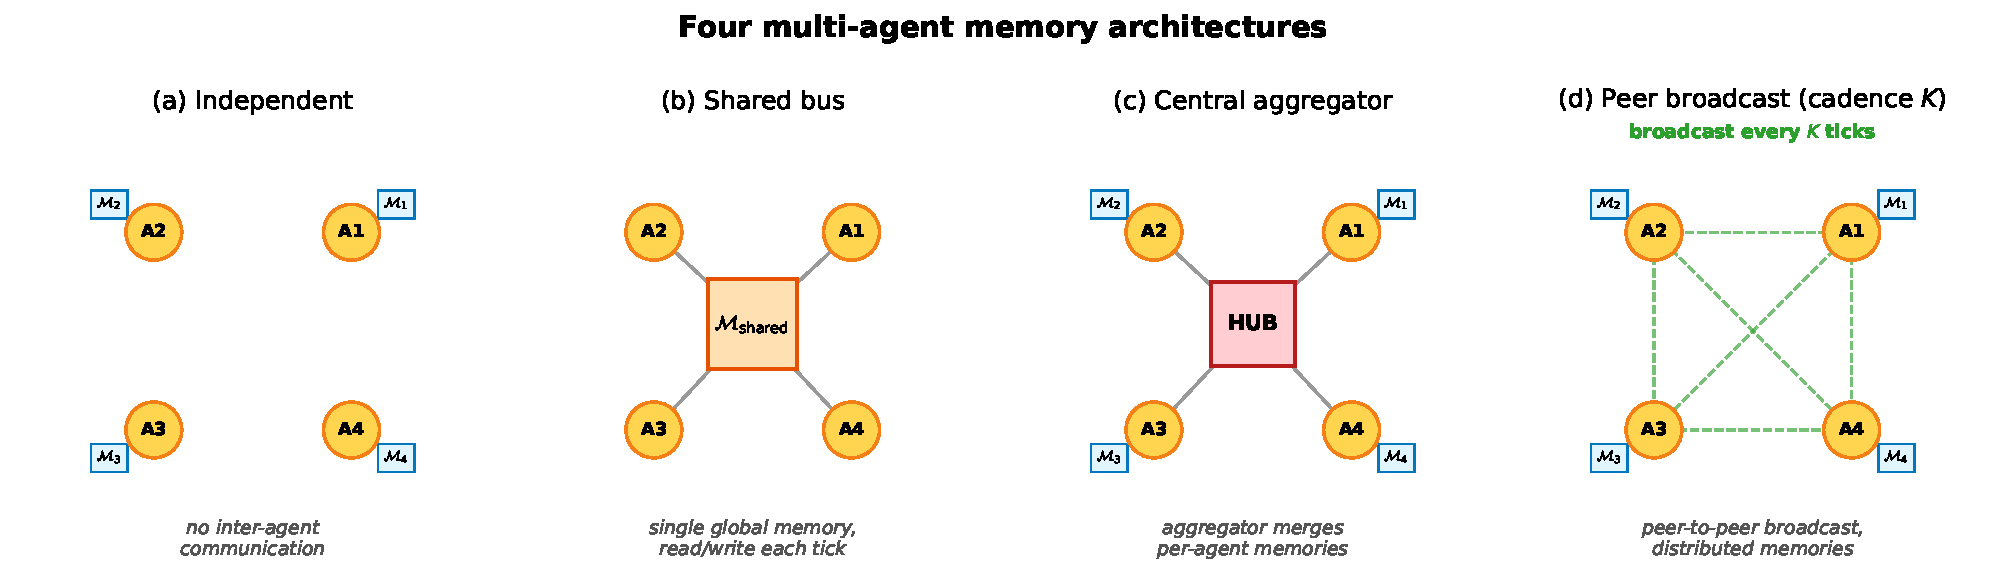
\includegraphics[width=\linewidth]{figures/fig_architectures.pdf}
  \caption{Четыре многоагентные архитектуры памяти. \textbf{(a)}~Независимая: приватная память на агента, без обмена. \textbf{(b)}~Общая шина: одна глобальная память, каждый агент читает/пишет каждый тик. \textbf{(c)}~Центральный агрегатор: памяти агентов плюс хаб, сливающий их в консенсусный отчёт. \textbf{(d)}~Широковещательная рассылка peer-to-peer: памяти агентов с попарным обменом снимками каждые $K$ тиков (ось каденции Эмпирического утверждения~1).}
  \label{fig:architectures}
\end{figure}

\begin{description}[leftmargin=10pt,topsep=2pt,itemsep=2pt]
\item[Независимая.] Каждый агент поддерживает приватное хранилище событий и граф понятий. Механизма межагентной коммуникации не существует. Бейзлайн-нижняя граница.
\item[Общая шина.] Все агенты публикуют наблюдения в единую шину событий \emph{коллективной памяти}. Один общий граф понятий перестраивается из объединения событий. Максимально централизовано.
\item[Центральный агрегатор (ConsensusLayer).] У каждого агента свой приватный граф понятий; центральный слой стягивает снимки и вычисляет слияние, взвешенное доверием, порождая единый \emph{консенсусный отчёт}, потребляемый всеми агентами.
\item[Широковещательная рассылка peer-to-peer (каденция $K$).] У каждого агента свой граф понятий и своё слитое представление. Каждые $K$ тиков каждый агент рассылает снимок в пассивную шину; каждый агент независимо сливает свой снимок с последним снимком, полученным от каждого пира. Разные агенты могут держать разные слитые представления; центрального отчёта нет.
\end{description}

Первые три соответствуют трём режимам в литературе по многоагентной
коммуникации: без обмена, агрегация в стиле CTDE и
децентрализованная пировая коммуникация. Четвёртая --- архитектура, к
которой Определение~2 и Эмпирическое утверждение~1 применимы
напрямую, поскольку каденция $K$ --- настраиваемый параметр, а не
фиксированный протокол. Механически $K$ --- это темп, с которым приватные
памяти консолидируются в коллективное представление, поэтому он и есть
структурная ось этой секции.

\subsection{Многоагентная факторизация}
\label{sec:multi-theory}

Расширим факторизацию на популяцию из $N$ агентов, разделяющих
информацию через коммуникационный протокол $\mathcal{C}_K$,
параметризованный каденцией рассылки $K$. Каждый агент $i$ имеет своё
состояние памяти $\mathcal{M}_i$ и выпускает свой запрос $q_i$. Пусть
$\mathcal{M}_i^{(K)}$ обозначает проекцию памяти агента $i$ в
момент запроса, после впитывания каждого пирового сообщения, полученного
при каденции $K$. Разделяются два канала связывания: (i) связывание
памяти $\mathcal{M}_{-i}^{(K)}$ --- последние снимки памяти пиров,
доступные агенту $i$; (ii) связывание занятости $\mathcal{O}_{-i}$ ---
множество целей, которые другие агенты уже заявили к моменту,
когда действует $i$.

\paragraph{Определение 2 (многоагентная оцениваемость стадий).}
Для каждого агента $i$
\[
P(C^\star_i \mid q_i, \mathcal{M}_i, \mathcal{C}_K)
=
P(Q^\star_i \mid q_i, \mathcal{M}_i)\;
P(R^\star_i \mid Q^\star_i, q_i, \mathcal{M}_i, \mathcal{M}_{-i}^{(K)})
\]
\[
\quad \cdot\;
P(M^\star_i \mid R^\star_i, q_i, \mathcal{M}_i, \mathcal{M}_{-i}^{(K)})\;
P(C^\star_i \mid M^\star_i, q_i, \mathcal{O}_{-i}).
\]
При многоагентном постадийно-марковском предположении
(Приложение~\ref{app:estimators}) четыре фактора оцениваемы из
поагентных логов траекторий, а эмпирико-частотные оценки
состоятельны.

\paragraph{Когда Определение~2 может нарушаться.}
Одноагентное постадийно-марковское свойство впитывает историю траектории в
$(q, \mathcal{M})$. В многоагентной постановке аналогичное
впитывание требует, чтобы зависимость от прошлых решений пиров входила только
через $\mathcal{M}_{-i}^{(K)}$ на стадии M и через
$\mathcal{O}_{-i}$ на стадии C. Этот шаг нетривиален:
$\mathcal{O}_{-i}$ суммирует занятость целей в момент решения, но
теряет информацию о том, \emph{как} пиры туда пришли.
Факторизация, следовательно, --- проекция на наблюдаемые поагентные
трассы при такой сводке. Возникают две конкретные моды нарушения: (i)
межагентные коммуникационные побочные каналы, не логируемые через
$\mathcal{C}_K$; (ii) координированные политики пиров, чьё решение на
стадии C зависит от скрытого состояния пиров, не суммируемого
$\mathcal{O}_{-i}$.

\subsection{Смещение бутылочного горлышка}
\label{sec:shift}

\paragraph{Эмпирическое утверждение~1 (смещение бутылочного горлышка M$\leftrightarrow$C, на уровне наклонов).}
Предположим дефицит ($N > T$ целей, см. \S\ref{sec:notation}) и
архитектуру пировой рассылки с каденцией $K \in \mathbb{N}$. Постулируются два
стилизованных предположения:
\textbf{(F)}~свежесть памяти $\nu(\mathcal{M}_{-i}^{(K)})$
поточечно не убывает при уменьшении $K$, и вероятность того, что
планировщик агента $i$ зафиксируется на достижимой цели, не убывает по
$\nu$;
\textbf{(O)}~вероятность того, что произвольная закоммиченная цель
уже находится в $\mathcal{O}_{-i}$, не возрастает при росте $K$.
Обозначим через $P(M^\star|R^\star;K)$ и $P(C^\star|M^\star;K)$
популяционные условные вероятности (усреднённые по агентам и
распределению сидов бенчмарка); $\hat{P}(\cdot)$ обозначает
соответствующую эмпирико-частотную оценку, вычисленную из логов. При
(F) и (O)
\[
\frac{\partial\, P(M^\star|R^\star;K)}{\partial K^{-1}} > 0,
\qquad
\frac{\partial\, P(C^\star|M^\star;K)}{\partial K^{-1}} < 0.
\]
Оба условия на наклоны --- прямые эмпирические предсказания,
проверяемые на логах через $\hat{P}$.

\paragraph{Чем это утверждение является и чем не является.}
Эмпирическое утверждение~1 --- \emph{утверждение об условных частотах на уровне наклонов}: каждый из двух наклонов проверяем и подтверждён на свипе из 35{,}640 прогонов (\S\ref{sec:multi-agent-results}) и независимо на свипе переносимости из 100 прогонов на стандартном MiniGrid (\S\ref{sec:limitations}). Мы сообщаем наклоны как \emph{размеры эффекта с кластерно-робастными доверительными интервалами} (ресемплированными по 81 независимой конфигурационной ячейке, а не по коррелированному числу прогонов) в Приложении~\ref{app:effect-sizes}. Граница утверждения относительно условного произведения $\Phi$ сформулирована один раз, в боксе «Границы применимости и не-утверждения» (\S1) и в \S\ref{sec:multi-agent-results}. Смещение --- сигнатура соперничества за дефицитные цели, а не устройства сетки: при изобилии ($T{>}N$) оба наклона выполаживаются, и антикорреляция M$\leftrightarrow$C ослабевает (Приложение~\ref{app:cadence-robustness}), т.е.\ предсказание ломается ровно там, где устранён механизм соперничества.

\paragraph{Хронология.}
Эмпирическое утверждение~1 является post-hoc. Оно было сформулировано \emph{после} первоначального свипа из 12{,}960 прогонов, проведённого при четырёх безразличных к стадиям гипотезах (Приложение~\ref{app:diagnostics}); затем два условия на наклоны были подтверждены на полном свипе из 35{,}640 прогонов, на масштабировании $N\!=\!12$ (Приложение~\ref{app:babyai}) и на обёртке переносимости MiniGrid (\S\ref{sec:limitations}). Мы заявляем это явно: подтверждённые знаки наклонов --- предсказания на укрупнённых данных, а не предварительно зарегистрированное
предсказание. Полностью формальная версия оставлена для будущей работы.

\subsection{Протокол свипа}
\label{sec:multi-agent-protocol}

Четыре архитектуры оцениваются на собственной многоагентной сетке ($12{\times}10$ клеток); каждый агент должен достичь клетки с тегом \texttt{water\_source}, выбирая действия через общий планировщик на основе памяти, так что различается только слой памяти. Свип скрещивает $N{\in}\{3,5,8\}$, $T{\le}N$, три раскладки (симметричная/асимметричная/случайная), три плотности опасностей, четыре архитектуры, восемь пировых каденций $K{\in}\{1,2,4,8,16,32,48,64\}$, 40 сидов --- 35{,}640 прогонов за $\approx 22$ мин на 8 ядрах. Логируются поагентные потиковые индикаторы Q/R/M/C (Приложение~\ref{app:estimators}); «звёздные» события уровня эпизода --- дизъюнкция по тикам. Отдельный блок оракульных интервенций на случаях дефицита $(N,T){\in}\{(3,2),(5,3),(8,5)\}$ при пяти каденциях оценивает оракульное R (память возвращает истинные позиции воды), оракульное M (планировщик фиксируется на ближайшей реальной воде) и оракульное C (завершение реальной материализованной фиксации гарантировано; Приложение~\ref{app:oracle-c-def}).

\subsection{Результаты: постадийная декомпозиция и смещение бутылочного горлышка}
\label{sec:multi-agent-results}

Свип из 35{,}640 прогонов излагается через четыре наблюдения,
структурированных зеркально Эмпирическому утверждению~1: (i) условная
декомпозиция изолирует стадии M и C как различающие
звенья; (ii) смещение бутылочного горлышка проявляется напрямую как отрицательная
внутрикаденционная корреляция между $P(M^\star|R^\star)$ и
$P(C^\star|M^\star)$, с пиком при $K\!=\!4$ и затуханием до шума при
$K\!=\!64$; (iii) на среднем времени до успеха результирующий компромисс
порождает внутренний оптимум при $K\!=\!8$ --- устойчивый по положению, но мелкий по запасу, с преимуществом над соседними быстрыми каденциями, не разрешённым при этом размере выборки (Приложение~\ref{app:effect-sizes}); (iv) на
условном произведении $\Phi$ тот же компромисс порождает монотонный
тренд, а не внутренний пик --- сводная статистика, о которой мы не делаем формальных утверждений. Бейзлайн с обученной коммуникацией и многоагентный
цикл оракульных интервенций закрывают подсекцию.

\subsubsection{Условная декомпозиция показывает, где отказывает каждая архитектура.}
Рисунок~\ref{fig:conditional-rates} показывает поархитектурные условные частоты Q/R/M/C; полная числовая картина с бутстреп-ДИ --- в Приложении~\ref{app:phi-detail}, Таблица~\ref{tab:multi-agent-cond}. Условная частота извлечения $P(R^\star|Q^\star)$ насыщена; различающий сигнал живёт на M и C. Общая шина, центральный агрегатор и быстрая пировая рассылка ($K\le4$) имеют высокое $P(M^\star|R^\star)$, но низкое $P(C^\star|M^\star)$; независимая и медленная пировая рассылка ($K\ge16$) показывают обратное --- компромисс M$\leftrightarrow$C, предсказанный Эмпирическим утверждением~1.

\begin{figure}[t]
  \centering
  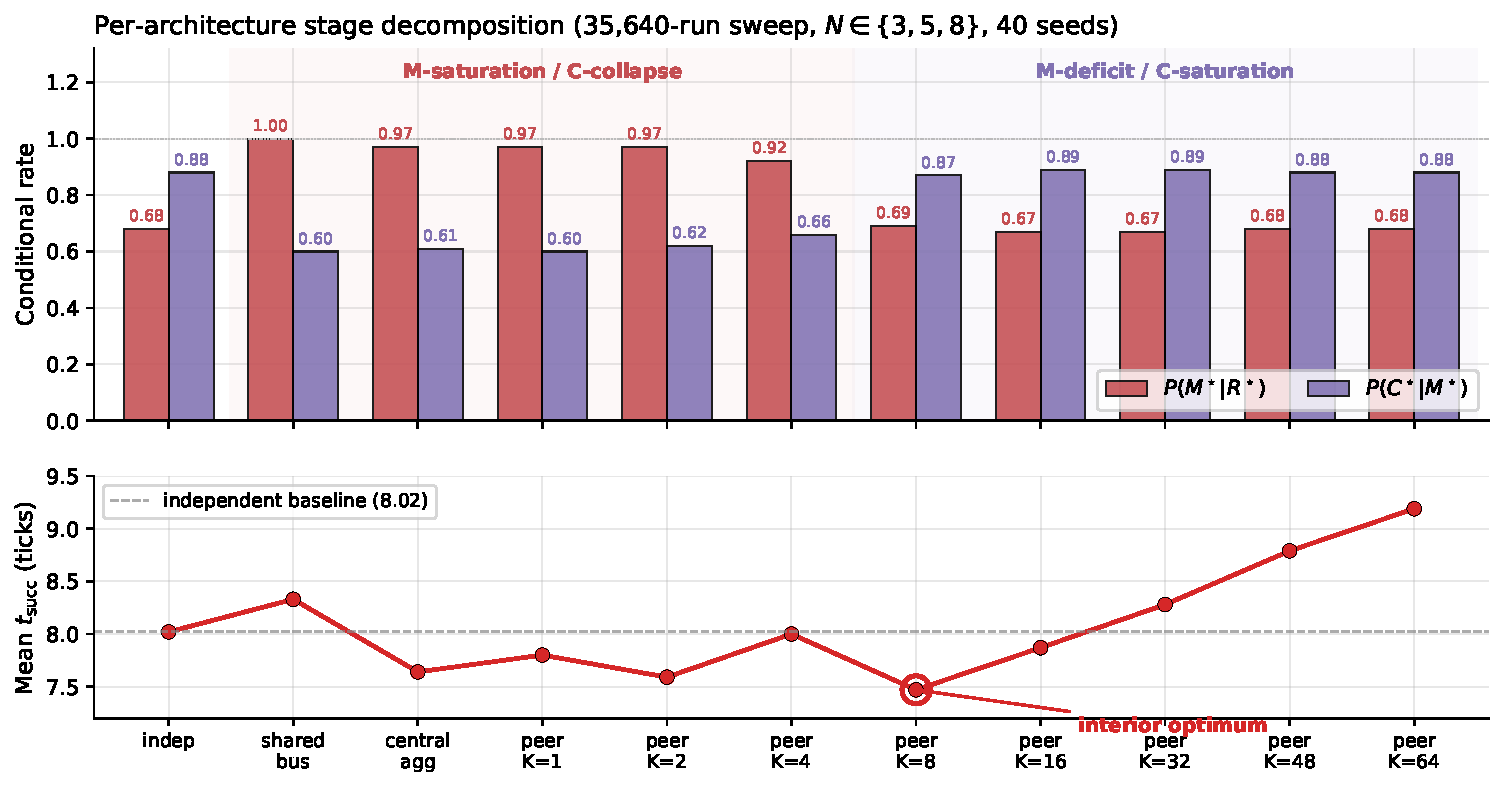
\includegraphics[width=\linewidth]{figures/fig_conditional_rates.pdf}
  \caption{Поархитектурные условные частоты (сверху) и среднее время до успеха (снизу) на свипе из 35{,}640 прогонов. Общая шина, центральный агрегатор и быстрая пировая рассылка ($K \le 4$) живут в режиме насыщения M / коллапса C; независимая и медленная пировая ($K \ge 16$) --- в режиме дефицита M / насыщения C. Среднее время до успеха имеет внутренний минимум при $K{=}8$ ($7.47$ тиков), ниже бейзлайна независимых агентов ($8.02$); положение устойчиво, но мелко --- запас над соседними быстрыми каденциями не разрешён (Приложение~\ref{app:effect-sizes}).}
  \label{fig:conditional-rates}
\end{figure}


\subsubsection{Смещение бутылочного горлышка и внутренний оптимум эффективности.}
По всем пировым прогонам Спирмен $P(M^\star|R^\star)$ от $K$ равен $-0.53$ (95\%-й кластерно-робастный ДИ $[-0.59,-0.47]$), а $P(C^\star|M^\star)$ от $K$ равен $+0.43$ (ДИ $[+0.37,+0.50]$); оба --- умеренные размеры эффекта, чьи ДИ исключают ноль при ресемплировании 81 конфигурационной ячейки (Приложение~\ref{app:effect-sizes}), что соответствует условиям на наклоны Эмпирического утверждения~1. Мы сообщаем именно их, а не $p$-значения, которые неинформативны при таком коррелированном размере выборки. Более сильная эмпирическая сигнатура --- на уровне отдельных конфигураций: Пирсон $P(M^\star|R^\star)$ от $P(C^\star|M^\star)$ \emph{внутри} фиксированного $K$ равен $-0.43, -0.54, -0.61, -0.19, -0.05, -0.04, -0.02, -0.02$ при $K{=}1,2,4,8,16,32,48,64$, с пиком при $K{=}4$ и затуханием до шума к $K{=}64$ (Рисунок~\ref{fig:jensen-scatter}, Приложение~\ref{app:phi-detail}). Конфигурации с высоким M систематически имеют низкое C: бутылочное горлышко мигрирует между двумя стадиями внутри одной и той же ячейки $(N,T,\text{раскладка},\text{опасность},\text{сид})$ при варьировании $K$. На метрике эффективности среднее $t_{\mathrm{succ}}$ имеет U-образную форму с внутренним минимумом при $K{=}8$ (7.47 тиков против 8.02 у независимого бейзлайна); положение минимума устойчиво, но мелко --- его запас над соседними быстрыми каденциями ($K{=}1,4$) не разрешён при ресемплировании на уровне ячеек (парно-бутстреповские ДИ в Приложениях~\ref{app:phi-detail} и \ref{app:effect-sizes}). Масштабирование до $N{=}12$ \emph{заостряет} сигнатуру: пиковый Пирсон растёт до $-0.70$ и
мигрирует наружу к $K\!=\!8$, что согласуется с тем, что более сильное связывание
занятости при большем $N$ задерживает переход между режимами издержек
(Приложение~\ref{app:babyai}, Рисунок~\ref{fig:scale-n12}).

\paragraph{Стратификация по провенансу: механизм за смещением.}
Аннотирование каждой фиксации $M^\star$ \emph{провенансом} свидетельств,
стоящих за ней, делает смещение бутылочного горлышка механизменным, а не
корреляционным. Пусть $\varphi$ --- чужая доля массы свидетельств,
поддерживающих зафиксированного кандидата, вычисленная из тех же весов
доверия/поддержки, которые использовало само слияние, и замороженная в момент фиксации; назовём фиксацию
\emph{варпом} (warp, $W^\star$), когда $\varphi \ge 0.8$: агент
коммитится на цель, которую знает по существу только от пиров. На
выделенном пировом свипе по ячейкам дефицита (случайные раскладки, 20
сидов, $K\in\{1,2,4,8,16\}$) доля варпов $P(W^\star|M^\star)$
падает с $0.55$ при $K{=}1$ до $0.11$ при $K{=}8$, тогда как страта
собственных свидетельств завершает на ровных $0.26$--$0.34$, а страта варпов
завершает ниже $0.05$ на всём диапазоне: \emph{C-коллапс
быстрого обмена сконцентрирован в страте варпов}. То, чем каденция
управляет механически, --- это какая часть материализации коллектива
работает на чужих свидетельствах, --- и именно эта страта проигрывает
гонку занятости. Та же стратификация
воспроизводится на непрерывном мосте VMAS ($0.72\to0.00$ по
$K{=}1/4/16$) и на текстовом LLM-субстрате ($0.42\to0.08$ по
$K{=}2/8$), причём кривые почти совпадают между субстратами. Полный
анализ, обусловленный провенансом (контрфактическая атрибуция маскированным
реплеем, замкнутая форма горизонта устаревания с зарегистрированным
hold-out $6/6$-exact и децентрализованный протокол починки), приведён в
сопутствующей рукописи; здесь стратификация служит
механизменным прочтением Эмпирического утверждения~1.

\paragraph{Чего мы не утверждаем о $\Phi$.} Условное произведение $\Phi = P(M^\star|R^\star)\!\cdot\!P(C^\star|M^\star)$ \emph{не} имеет внутреннего пика в проверенном диапазоне (оценка средним произведений монотонно растёт от $0.569$ при $K{=}4$ до $0.603$ при $K{=}64$, сходясь к границе независимых агентов $0.605$). Утверждение уровня наклонов Эмпирического утверждения~1 --- об условных частотах самих по себе, не о $\Phi$; мы не делаем формальных утверждений о форме $\Phi(K)$. Детали разрыва Йенсена и сравнение POM--MOP --- в Приложении~\ref{app:phi-detail}.

\paragraph{Бейзлайн с обученной коммуникацией: стадийные события структурно вырождены даже при конкурентоспособном успехе.}
Политика в стиле CommNet \citep{sukhbaatar2016commnet}, обученная PPO~\citep{schulman2017proximal} на том же сценарии ($N{=}3$, $T{=}2$), достигает $0.667$ успеха на отложенной выборке ($n{=}100$ сидов) --- вровень с символьной пировой архитектурой при $K{=}8$ ($0.65$). Несмотря на это, профиль Q/R/M/C остаётся структурно вырожденным: $Q^\star{=}1.00$ насыщено по построению; $R^\star{=}0.997$, $M^\star{=}0.997$ схлопнуты вместе ($P(M^\star|R^\star){=}1.00$). Это и есть проверенное структурное утверждение: вещественный коммуникационный вектор никогда не бывает информативно пустым (Q насыщается) и лишён явного интерфейса фиксации цели (R/M сливаются), независимо от бюджета обучения. Многоагентный аналог одноагентного анализа обученного BC (\S\ref{sec:single-results}). Полная архитектура, гиперпараметры PPO и параллельное сравнение REINFORCE и PPO --- в Приложении~\ref{app:learned-baselines}.

\paragraph{Свип LLM-моделей: логгер локализует реальный отказ в языковых агентах.}
Таблица~\ref{tab:llm-smoke} прогоняет тот же контракт событий Q/R/M/C на двух локальных LLM-агентах (qwen3:4b и llama3.1 через Ollama) на TextNav, свипуя бюджет шагов по $\{6,12,25\}$ ($8$ эпизодов каждый; задача требует $\sim$10 низкоуровневых шагов). При щедром бюджете ($12$, $25$) оба агента успешны, и все четыре стадии срабатывают. При бюджете ниже требуемого ($6$) успех падает до $0/8$ у \emph{обеих} моделей --- и декомпозиция показывает, \emph{где}: $Q^\star{=}R^\star{=}M^\star{=}1.00$ (агенты формируют запрос, извлекают и фиксируют правильную цель в каждом эпизоде), тогда как $C^\star{=}0.00$ (ни один не завершает вовремя). Фреймворк локализует отказ точно в ограниченном бюджетом завершении ($C$), а не в формировании запроса, извлечении или материализации; то, что обе модели отказывают одинаково, показывает структурность отказа, а не артефакт модели. Это то самое диагностическое свойство, которое фреймворк заявляет, теперь продемонстрированное на \emph{реальных языковых агентах}: в остальном непрозрачный коллапс успеха ($1.00\to0.00$) разрешается в конкретную отказывающую стадию. (Замечание об инструментировании: наивный вызов chat-шаблона qwen3:4b/Ollama изначально возвращал пустые строки \texttt{response}, потому что модель тратила короткий бюджет структурированного вывода в отдельном поле размышлений; для qwen3:4b мы используем сырой structured completion и парсер первой строки, что зафиксировано для воспроизводимости.)

\paragraph{Многоагентная феноменология воспроизводится на живом LLM-коллективе.}
Помимо одноагентного исследования бюджета, тот же контракт событий
инструментирует коллектив из $N{=}3$ LLM-агентов (llama3.1), разделяющих
символьную память мест пировой рассылкой при дефиците ($M{=}2$
доступные для захвата цели, четыре раскладки, $K\in\{2,8\}$), причём все предсказания
зарегистрированы до прогонов. Каденционная феноменология из
\S\ref{sec:multi-agent-results} переносится на языковой
субстрат: парное сравнение с бейзлайном без коммуникации
на идентичных раскладках показывает, что сырой обмен \emph{снижает} успех с
$2/3$ до $1/3$ на эпизод --- C-коллапс гонки за занятость, теперь
порождённый агентами, чьи запросы, извлечение тегов и коммиты
сделаны LLM, --- а столкновения целей появляются в $7/8$ эпизодов с общей
памятью. Присоединение протокола починки «резервирование и откат»
(конструктивный ответ на открытую проблему~3 из
Приложения~\ref{app:open-problems}) возвращает часть потери
($0.333\to0.417$ при обеих каденциях, латентность отката снова
${\approx}K$). Два интерфейсных наблюдения переносятся на любой
дизайн LLM-поверх-символьной-памяти: LLM-формирователи запросов свободно генерируют
теги извлечения вне словаря памяти (что требует толерантных
гейтов извлечения), а малые локальные модели надёжны в семантическом
коммите, но не в координатной арифметике или систематическом исследовании
(что требует слоёного исполнения). Полный протокол и анализ провенанса ---
в сопутствующей рукописи.

Границы: это контролируемые исследования на локальных моделях; масштабирование того же контракта на полноценных агентов в стиле Voyager/MemGPT на более богатых задачах с несколькими модами отказа развивается далее (валидация на внешних фреймворках) и в Приложении~\ref{app:sota-coverage}.

\begin{table}[h]
  \caption{Свип бюджета шагов LLM TextNav: Q/R/M/C локализует ограниченный завершением отказ у двух локальных Ollama-агентов. Восемь эпизодов на (модель, лимит шагов), температура 0.0; задача требует $\sim$10 низкоуровневых шагов. При бюджете ниже этого требования (лимит шагов 6) успех падает до $0.00$ у обеих моделей, однако $Q^\star{=}R^\star{=}M^\star{=}1.00$ (агенты формируют запрос, извлекают и фиксируют правильную цель в каждом эпизоде), тогда как $C^\star{=}0.00$: фреймворк локализует отказ на стадии C, а не на Q/R/M. Обе модели ведут себя идентично, так что отказ структурен (бюджет), а не специфичен для модели. Артефакты: \texttt{tmp/llm\_steplimit\_\{6,12,25\}}.}
  \label{tab:llm-smoke}
  \centering
  \small
  \begin{tabular}{l c c c c c c}
    \toprule
    Модель & Лимит шагов & Успех & $Q^\star$ & $R^\star$ & $M^\star$ & $C^\star$ \\
    \midrule
    qwen3:4b & 6  & 0.00 & 1.00 & 1.00 & 1.00 & \textbf{0.00} \\
    llama3.1 & 6  & 0.00 & 1.00 & 1.00 & 1.00 & \textbf{0.00} \\
    \midrule
    qwen3:4b & 12 & 1.00 & 1.00 & 1.00 & 1.00 & 1.00 \\
    llama3.1 & 12 & 1.00 & 1.00 & 1.00 & 1.00 & 1.00 \\
    qwen3:4b & 25 & 1.00 & 1.00 & 1.00 & 1.00 & 1.00 \\
    llama3.1 & 25 & 1.00 & 1.00 & 1.00 & 1.00 & 1.00 \\
    \bottomrule
  \end{tabular}
\end{table}

\paragraph{Многоагентные оракульные интервенции замыкают цикл диагностика$\to$интервенция$\to$верификация.}
На случаях дефицита среднее $t_{\mathrm{succ}}$ при малой/промежуточной каденции ($K{\in}\{1,2,4\}$) падает с $\sim10$--$11$ в бейзлайне до $\sim7.2$ при оракульном R или оракульном M и далее до $\sim6.1$ при оракульном C, которое дополнительно устраняет путь после фиксации; при медленной каденции ($K{=}16$) бейзлайн уже в пределах $\sim1.2$ от пола R/M-оракулов (Таблица~\ref{tab:multi-agent-oracle} в Приложении~\ref{app:multi-oracle}). Существенно, что оракульное C даёт наибольшее сокращение времени, но наименьший прирост доли успеха (Приложение~\ref{app:oracle-c-def}): при дефиците завершение стоит времени, тогда как извлечение и материализация решают успех. Индуцированное каденцией избыточное время при малых/промежуточных $K$ атрибутируется переходу M$\leftrightarrow$C; при больших $K$ бутылочное горлышко перемещается в одиночное исследование.

Многоагентный блок тем самым доставляет свою половину аргумента.
Каденция $K$ --- механически темп, с которым приватные памяти
консолидируются в коллективное представление; данные показывают, что у этого темпа есть
нетривиальный внутренний оптимум ($K\!=\!8$ на $t_{\mathrm{succ}}$), что
его канал издержек --- связывание занятости, и что оба эффекта
видимы постадийно на той же цепочке Q/R/M/C, что и для одиночных
агентов. Консолидация --- не только одноагентный предел; в
коллективе это настраиваемая, измеримая ось дизайна.

\section{Контракт на сторонних агентных стеках}
\label{sec:external}

Самый сильный вопрос о внешней валидности, который читатель может задать
диагностическому протоколу, --- работает ли он на системах, которые его авторы не
строили. Поэтому мы инструментируем три сторонних агентных стека --- цикл
function-calling на OpenAI SDK, преднастроенный ReAct-агент
LangGraph и пару AssistantAgent/UserProxy из AutoGen, все на одной
локальной модели (llama3.1, температура $0$) --- идентичным
контрактом Q/R/M/C, определённым однократно над \emph{трассами инструментов}: эпизодическая
бытовая память открывается через инструменты \method{recall}/\method{goto}/%
\method{take}, и $Q^\star$ срабатывает при запросе к памяти, $R^\star$ ---
при \emph{атрибуции} (возвращённая запись называет предмет в его истинном
месте), $M^\star$ --- при фиксации уровня эпизода (\method{goto} к
истинному месту, в верности Определению~1; дисциплина первого коммита (first-commitment discipline)
$M_1$ логируется как вспомогательная диагностика качества фиксации), а
$C^\star$ --- при завершении задачи в пределах бюджета инструментов. Три варианта
инженерят по одному отказу каждый --- консолидационный разрыв (consolidation gap; факт о местоположении
никогда не был записан в память), неоднозначность с устаревшим дистрактором, бюджет
инструментов ниже требований задачи --- плюс чистый контроль; все
предсказания были зарегистрированы до прогонов, а две ревизии
семантики событий (утечка атрибуции; перетянутое $M^\star$)
зафиксированы в регистрационном файле.

\begin{table}[h]
\caption{Q/R/M/C на трёх сторонних агентных фреймворках (llama3.1,
20 эпизодов на ячейку, идентичные эпизоды/инструменты/бюджеты). Структурные
отказы локализуются везде идентично: консолидационный разрыв ---
$R{=}0.00$, а бюджетный отказ --- $C{=}0.00$ при $Q{=}R{=}1$ для
всех трёх стеков. На \emph{чистом} контроле фреймворки расходятся
от $0.50$ до $0.75$ сквозным образом --- и декомпозиция атрибутирует
этот разброс (см. текст). $M_1$: первый \method{goto} целится в истинное
место; stale$_1$: первый \method{goto} целится в устаревший дистрактор.}
\label{tab:external}
\centering
\small
\begin{tabular}{llcccccc}
\toprule
Фреймворк & Вариант & $Q^\star$ & $R^\star$ & $M^\star$ & $C^\star$ & $M_1$ & stale$_1$ \\
\midrule
OpenAI SDK & контроль     & 1.00 & 1.00 & 0.85 & 0.75 & 0.25 & --- \\
           & консолидац. разрыв & 1.00 & \textbf{0.00} & 0.50 & 0.40 & 0.25 & --- \\
           & устаревшая неоднозн.   & 1.00 & 1.00 & 0.90 & 0.30 & 0.25 & 0.20 \\
           & жёсткий бюджет      & 1.00 & 1.00 & 0.25 & \textbf{0.00} & 0.25 & --- \\
\midrule
LangGraph  & контроль     & 1.00 & 1.00 & 0.70 & 0.50 & 0.50 & --- \\
           & консолидац. разрыв & 1.00 & \textbf{0.00} & 0.20 & 0.15 & 0.10 & --- \\
           & устаревшая неоднозн.   & 1.00 & 1.00 & 0.65 & 0.60 & 0.50 & 0.35 \\
           & жёсткий бюджет      & 1.00 & 1.00 & 0.10 & \textbf{0.00} & 0.10 & --- \\
\midrule
AutoGen    & контроль     & 1.00 & 1.00 & 0.85 & 0.55 & 0.45 & --- \\
           & консолидац. разрыв & 1.00 & \textbf{0.00} & 0.30 & 0.20 & 0.15 & --- \\
           & устаревшая неоднозн.   & 1.00 & 1.00 & 0.50 & 0.45 & 0.35 & 0.40 \\
           & жёсткий бюджет      & 1.00 & 1.00 & 0.15 & \textbf{0.00} & 0.15 & --- \\
\bottomrule
\end{tabular}
\end{table}

\begin{figure}[t]
\centering
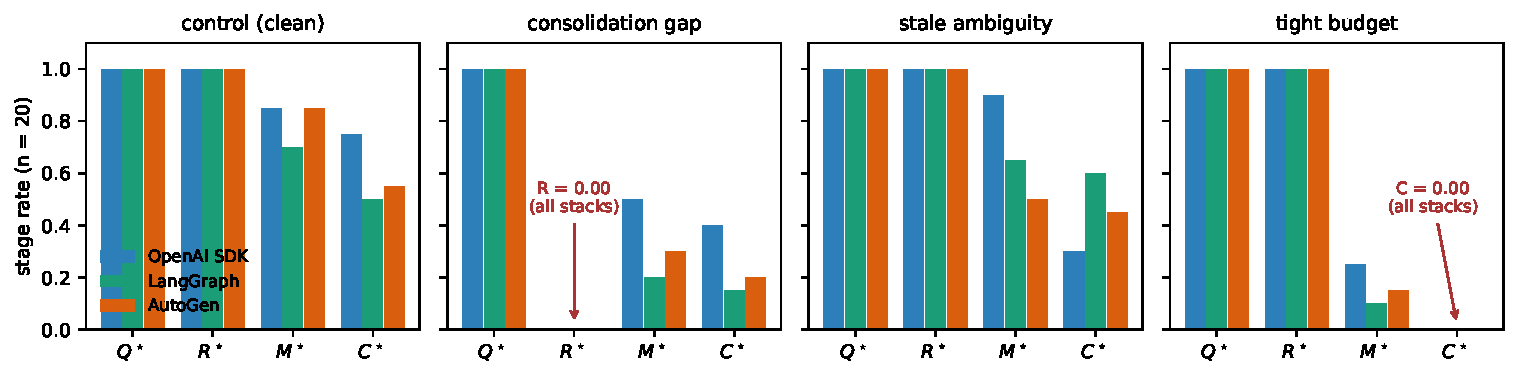
\includegraphics[width=\linewidth]{figures/fig_external_stages}
\caption{Постадийные профили трёх сторонних агентных стеков на четырёх
инженерных вариантах (llama3.1, $n{=}20$ на ячейку). Запрос и извлечение
насыщаются везде идентично; два структурных отказа дают
точные нулевые столбцы на каждом стеке ($R^\star{=}0$ при
консолидационном разрыве, $C^\star{=}0$ при жёстком бюджете);
поведенческий разброс между фреймворками целиком живёт на стадиях M и
C.}
\label{fig:external-stages}
\end{figure}

Три наблюдения (Таблица~\ref{tab:external},
Рисунок~\ref{fig:external-stages}). \textbf{(1)~Структурные
локализации точны и независимы от фреймворка.} Когда в памяти
нет факта, $R^\star{=}0.00$ на каждом стеке; когда бюджет
не вмещает завершение, $C^\star{=}0.00$ при $Q^\star{=}R^\star{=}1$ на
каждом стеке ($20/20$ эпизодов в каждом). Контракт не требует
пофреймворковой адаптации. \textbf{(2)~Чистый контроль разделяет
фреймворки, и декомпозиция говорит как.} Сквозной успех на
ОДНИХ И ТЕХ ЖЕ чистых эпизодах лежит в диапазоне от $0.50$ (LangGraph) до $0.75$ (OpenAI SDK).
Лидерборд сообщил бы «разное качество»; стадии показывают
общую патологию плюс разную экономику циклов: дисциплина первого
коммита слаба везде ($M_1{=}0.25$--$0.50$ --- первый
\method{goto} агента часто игнорирует его же только что извлечённые
свидетельства), материализация уровня эпизода восстанавливается до $0.70$--$0.85$
через циклы переспроса, а затем фреймворки различаются тем, какая часть
этого восстановления доживает до завершения ($C^\star/M^\star$ от $0.88$
у цикла OpenAI SDK до $0.65$ у AutoGen). \textbf{(3)~Устаревший
дистрактор тянет, измеримо и неравномерно.} Устаревшая запись
захватывает первый коммит в $0.20$--$0.40$ неоднозначных эпизодов
(сильнее всего у AutoGen), и цена её для завершения
специфична фреймворку: цикл OpenAI SDK платит тяжелее всех
($C^\star:0.75\to0.30$), тогда как LangGraph и AutoGen поглощают крюк
($0.50\to0.60$; $0.55\to0.45$) --- LLM-памятный аналог
гейтинга по устареванию, решающую роль которого показали коллективные
эксперименты. Честно проваленные регистрации: поведенческие предсказания,
предполагавшие чистый контроль (все стадии $\ge 0.75$; равномерное
индуцированное неоднозначностью падение завершения), сломались \emph{потому что сами фреймворки
проваливают чистую задачу на память в 25--50\% случаев и платят за
неоднозначность в разных местах} --- а это и есть наблюдения (2)--(3), не
шум; все ревизии зафиксированы как зарегистрированные провалы с
механизмами. Границы: три стека при $n{=}20$ на ячейку на одной основной
модели; Letta/CrewAI (Python $\ge$3.10) и модели API-масштаба --- естественное
расширение.

\section{Ограничения и будущая работа}
\label{sec:limitations}

\textbf{Переносимость между субстратами: условия на наклоны выполняются на MiniGrid.} Условия на наклоны Эмпирического утверждения~1 выполняются и на субстрате стандартного MiniGrid. Многоагентная обёртка на основе FourRooms (построенная из \texttt{minigrid.core.grid.Grid} + примитивов Wall/Floor/Lava, идентичные операциональные определения $Q^\star,R^\star,M^\star,C^\star$; \texttt{experiments/minigrid\_multiagent\_wrapper/}) использована для свипа переносимости из 100 прогонов ($K{\in}\{1,4,8,16,64\}$, 20 сидов, $N{=}3$, $T{=}2$): Спирмен $P(M^\star|R^\star)$ от $K$ равен $-0.50$, а Спирмен $P(C^\star|M^\star)$ от $K$ равен $+0.50$ (умеренные ранговые корреляции; это малый свип из 100 прогонов, поэтому мы сообщаем размеры эффекта и не опираемся на значимость). Внутренний минимум $t_{\mathrm{succ}}$ не отделяется при этом минимальном размере свипа (5 каденций, 20 сидов, одна плотность опасностей); более плотный свип --- естественный следующий шаг. Шов между двумя субстратами тем самым закрыт на уровне утверждения о наклонах.

\textbf{Эмпирическое утверждение~1 --- только об условных частотах на уровне наклонов.} Два условия на наклоны выполняются как умеренные, кластерно-робастные размеры эффекта (Приложение~\ref{app:effect-sizes}); мы не делаем формальных утверждений о форме условного произведения $\Phi$ (\S\ref{sec:shift}). Будущая формулировка непосредственно в терминах поверхности временн\'{ы}х издержек или вывод при генеративной модели (пуассоновски-обновляемая память, занятость рождения-гибели) превратили бы эмпирическое утверждение в теорему.

\textbf{Оцениваемость при скрытом состоянии.} При нелогируемых внутриэпизодных переписываниях запросов или пировых побочных каналах Определения~1 и~2 --- проекции на залогированные трассы, а не полная идентификация.

\textbf{Общая система координат.} Все многоагентные результаты предполагают, что агенты
интерпретируют места в общей системе координат: межагентная идентичность
места --- это координатная близость, с семантическими профилями как
разрешителем ничьих внутри пространственного радиуса. Проблема соответствия мест ---
обозначают ли записи двух агентов вообще одно и то же место ---
здесь, следовательно, вынесена за скобки, а не решена. Сопутствующая рукопись снимает
это предположение конструктивно (идентичность мест на основе отпечатков с
консенсусным восстановлением системы координат с точностью до трансляции и поворота на $90^\circ$)
и показывает, что измерения Q/R/M/C, включая каденционные наклоны и
горизонт устаревания, неизменны поверх восстановленных систем координат; более трудные
варианты (непрерывное $SE(2)$, шум внешнего вида, выравнивание
символов) остаются открытыми.

\textbf{Обученные бейзлайны.} Бейзлайн CommNet PPO достигает успеха $0.667$ на сценарии дефицита --- конкурентоспособно с символьным пировым при $K{=}8$ ($0.65$) --- и подтверждает Q-насыщение ($Q^\star{=}1.00$) и коллапс R/M ($P(M^\star|R^\star){=}1.00$) при конкурентоспособном успехе. Структурное предсказание теперь подтверждено, а не постулировано; абляции на архитектурах с явными символьными каналами фиксации цели оставлены для будущей работы.

\textbf{Масштаб.} Многоагентный свип ограничен $N{=}12$ (Приложение~\ref{app:babyai}; сигнатура заостряется, пиковый Пирсон $-0.70$ при $K{=}8$, внутренний минимум $t_{\mathrm{succ}}$ $4.77$). Более плотное масштабирование при $N{\ge}16$ --- будущая работа.
\textbf{Непрерывный субстрат.} Предварительная проверка VMAS~\citep{bettini2022vmas} воспроизводит \emph{оба} знака наклонов Эмпирического утверждения~1 в режиме связывания (Спирмен $-1.00$ и $+1.00$ по $K{\le}16$, 40 сидов; Приложение~\ref{app:vmas}), переиспользуя символьную память через мост дискретизации. Это лишь направленный сигнал --- идеальная ранговая корреляция по пяти монотонным точкам, одна конфигурация, дискретизованная память, --- так что он указывает, что смещение не является артефактом клеток сетки, но полная валидация в непрерывном пространстве состояний с кластерно-робастными ДИ остаётся будущей работой.

\section{Более широкое влияние}

Статья предлагает диагностическое оценивание для агентов на основе памяти в симулированной навигации. Её положительное влияние методологично: сделать отказы на основе памяти более измеримыми между архитектурами и сделать ось каденции распределённой многоагентной памяти настраиваемой по эмпирически обоснованному критерию. Потенциальные негативные влияния косвенны и возникли бы, если бы похожая диагностика использовалась для улучшения агентов в критичных к безопасности постановках (рои дронов, автономные транспортные средства, распределённые сенсорные сети) без адекватных мер защиты. Настоящая работа --- инфраструктура уровня бенчмарка, а не готовая к развёртыванию система.

\section{Заключение}

Мы предложили Q/R/M/C --- четырёхстадийную декомпозицию навигации на основе
памяти, чьи факторы оцениваемы из стандартных логов траекторий, ---
и использовали её как диагностический инструмент на символьных, обученных,
LLM-управляемых, одноагентных и многоагентных трассах. Главный результат ---
не новая архитектура агента: это воспроизводимый протокол логирования и
оценивания, разделяющий формирование запроса, удовлетворение
извлечения, материализацию цели и завершение после извлечения.
По всем экспериментам этот протокол локализует отказы, которые
оценивание «только успех» не может, обнажает вырожденную наблюдаемость у
неявных обученных политик и делает каденцию обмена памятью измеримой
как постадийная переменная дизайна.

\begin{ack}
Рукопись подготовлена в анонимизированной форме для рецензирования.
Представленные эксперименты выполнены из единого бенчмаркового конвейера,
экспортирующего сводки по семействам задач, сравнения ассиста вкл/выкл, диагностику
методов, CSV многоагентных свипов и бутстреп-анализы из
одних и тех же эталонных бенчмарковых артефактов.
\end{ack}

{\small
\begin{thebibliography}{9}

\bibitem[Andrychowicz et~al.(2017)]{andrychowicz2017hindsight}
M.~Andrychowicz, F.~Wolski, A.~Ray, J.~Schneider, R.~Fong, P.~Welinder, B.~McGrew, J.~Tobin, P.~Abbeel, and W.~Zaremba.
\newblock Hindsight experience replay.
\newblock In \emph{NeurIPS}, 2017.

\bibitem[B\v{e}lohl\'avek(1999)]{belohlavek1999fuzzy}
R.~B\v{e}lohl\'avek.
\newblock Fuzzy Galois connections.
\newblock \emph{Mathematical Logic Quarterly}, 45(4):497--504, 1999.

\bibitem[Bettini et~al.(2022)]{bettini2022vmas}
M.~Bettini, R.~Kortvelesy, J.~Blumenkamp, and A.~Prorok.
\newblock VMAS: A vectorized multi-agent simulator for collective robot learning.
\newblock In \emph{16th International Symposium on Distributed Autonomous Robotic Systems (DARS)}, 2022.
\newblock arXiv:2207.03530.

\bibitem[Boyd et~al.(2006)]{boyd2006gossip}
S.~Boyd, A.~Ghosh, B.~Prabhakar, and D.~Shah.
\newblock Randomized gossip algorithms.
\newblock \emph{IEEE Trans.\ Information Theory}, 52(6):2508--2530, 2006.

\bibitem[Chevalier-Boisvert et~al.(2018)]{chevalier2018babyai}
M.~Chevalier-Boisvert, D.~Bhoopchand, H.~Abdolmaleki, and A.~Mordatch.
\newblock BabyAI: A platform to study the sample efficiency of grounded language learning.
\newblock In \emph{ICLR}, 2019.

\bibitem[Chevalier-Boisvert et~al.(2023)]{MinigridMiniworld23}
M.~Chevalier-Boisvert, B.~Lahlou, S.~Willems, and P.~S. Castro.
\newblock MiniGrid and MiniWorld: Modular reinforcement learning environments.
\newblock \emph{arXiv:2306.13831}, 2023.

\bibitem[Chhikara et~al.(2025)]{chhikara2025mem0}
P.~Chhikara, D.~Khant, S.~Aryan, T.~Singh, and D.~Yadav.
\newblock Mem0: Building production-ready AI agents with scalable long-term memory.
\newblock \emph{arXiv:2504.19413}, 2025.

\bibitem[Dayan(1993)]{dayan1993improving}
P.~Dayan.
\newblock Improving generalization for temporal difference learning: The successor representation.
\newblock \emph{Neural Computation}, 5(4):613--624, 1993.

\bibitem[Deitke et~al.(2022)]{deitke2022procthor}
M.~Deitke, E.~V. Wijmans, D.~Schwenk, O.~Salvador, K.~M. Ehsani, et al.
\newblock ProcTHOR: Large-scale embodied AI using procedural generation.
\newblock In \emph{NeurIPS Datasets and Benchmarks}, 2022.

\bibitem[Efron(1979)]{efron1979bootstrap}
B.~Efron.
\newblock Bootstrap methods: Another look at the jackknife.
\newblock \emph{Annals of Statistics}, 7(1):1--26, 1979.

\bibitem[Foerster et~al.(2016)]{foerster2016learning}
J.~N. Foerster, Y.~M. Assael, N.~de~Freitas, and S.~Whiteson.
\newblock Learning to communicate with deep multi-agent reinforcement learning.
\newblock In \emph{NeurIPS}, 2016.

\bibitem[Foerster et~al.(2018)]{foerster2018ctde}
J.~N. Foerster, G.~Farquhar, T.~Afouras, N.~Nardelli, and S.~Whiteson.
\newblock Counterfactual multi-agent policy gradients.
\newblock In \emph{AAAI}, 2018.

\bibitem[Ganter and Wille(1999)]{ganter1999fca}
B.~Ganter and R.~Wille.
\newblock \emph{Formal Concept Analysis: Mathematical Foundations}.
\newblock Springer, 1999.

\bibitem[Ghosh et~al.(2021)]{ghosh2021learning}
D.~Ghosh, A.~Gupta, A.~Reddy, J.~Fu, S.~Levine, and C.~Finn.
\newblock Learning to reach goals via iterated supervised learning.
\newblock In \emph{ICLR}, 2021.

\bibitem[Gigerenzer and Goldstein(1996)]{gigerenzer1996reasoning}
G.~Gigerenzer and D.~G. Goldstein.
\newblock Reasoning the fast and frugal way: Models of bounded rationality.
\newblock \emph{Psychological Review}, 103(4):650--669, 1996.

\bibitem[Gupta et~al.(2017)]{gupta2017cognitive}
S.~Gupta, J.~Davidson, S.~Levine, R.~Sukthankar, and J.~Malik.
\newblock Cognitive mapping and planning for visual navigation.
\newblock In \emph{CVPR}, 2017.

\bibitem[Holm(1979)]{holm1979simple}
S.~Holm.
\newblock A simple sequentially rejective multiple test procedure.
\newblock \emph{Scandinavian Journal of Statistics}, 6(2):65--70, 1979.

\bibitem[Kolve et~al.(2017)]{kolve2017ai2thor}
E.~Kolve, R.~Mottaghi, D.~Gordon, Y.~Zhu, A.~Gupta, A.~Farhadi, and D.~Fox.
\newblock AI2-THOR: An interactive 3D environment for visual AI.
\newblock \emph{arXiv:1712.05474}, 2017.

\bibitem[Kuipers(2000)]{kuipers2000spatial}
B.~Kuipers.
\newblock The spatial semantic hierarchy.
\newblock \emph{Artificial Intelligence}, 119(1--2):191--233, 2000.

\bibitem[Lieder and Griffiths(2020)]{lieder2020resource}
F.~Lieder and T.~L. Griffiths.
\newblock Resource-rational analysis: Understanding human cognition as the optimal use of limited computational resources.
\newblock \emph{Behavioral and Brain Sciences}, 43:e1, 2020.

\bibitem[Lowe et~al.(2017)]{lowe2017maddpg}
R.~Lowe, Y.~Wu, A.~Tamar, J.~Harb, P.~Abbeel, and I.~Mordatch.
\newblock Multi-agent actor-critic for mixed cooperative-competitive environments.
\newblock In \emph{NeurIPS}, 2017.

\bibitem[Mac~Lane(1998)]{maclane1998categories}
S.~Mac~Lane.
\newblock \emph{Categories for the Working Mathematician}.
\newblock Springer, 2nd edition, 1998.

\bibitem[Momennejad et~al.(2017)]{momennejad2017successor}
I.~Momennejad, E.~M. Russek, J.~H. Cheong, M.~M. Botvinick, N.~Daw, and S.~J. Gershman.
\newblock The successor representation in human reinforcement learning.
\newblock \emph{Nature Human Behaviour}, 1:680--692, 2017.

\bibitem[O'Keefe and Nadel(1978)]{okeefe1978hippocampus}
J.~O'Keefe and L.~Nadel.
\newblock \emph{The Hippocampus as a Cognitive Map}.
\newblock Oxford University Press, 1978.

\bibitem[Packer et~al.(2023)]{packer2023memgpt}
C.~Packer, V.~Fang, S.~Patil, K.~Lin, S.~Wooders, and J.~Gonzalez.
\newblock MemGPT: Towards LLMs as operating systems.
\newblock \emph{arXiv:2310.08560}, 2023.

\bibitem[Park et~al.(2023)]{park2023generative}
J.~S. Park, J.~C. O'Brien, C.~J. Cai, M.~R. Morris, P.~Liang, and M.~S. Bernstein.
\newblock Generative agents: Interactive simulacra of human behavior.
\newblock \emph{arXiv:2304.03442}, 2023.

\bibitem[Rashid et~al.(2018)]{rashid2018qmix}
T.~Rashid, M.~Samvelyan, C.~Schroeder de Witt, G.~Farquhar, J.~Foerster, and S.~Whiteson.
\newblock QMIX: Monotonic value function factorisation for deep multi-agent reinforcement learning.
\newblock In \emph{ICML}, 2018.

\bibitem[Savinov et~al.(2018)]{savinov2018semi}
N.~Savinov, A.~Dosovitskiy, and V.~Koltun.
\newblock Semi-parametric topological memory for navigation.
\newblock In \emph{ICLR}, 2018.

\bibitem[Savva et~al.(2019)]{savva2019habitat}
M.~Savva, A.~Kadian, O.~Maksymets, Y.~Zhao, E.~Wijmans, B.~Jain, J.~Straub, J.~Liu, V.~Koltun, J.~Malik, et al.
\newblock Habitat: A platform for embodied AI research.
\newblock In \emph{ICCV}, 2019.

\bibitem[Schulman et~al.(2016)]{schulman2016gae}
J.~Schulman, P.~Moritz, S.~Levine, M.~Jordan, and P.~Abbeel.
\newblock High-dimensional continuous control using generalized advantage estimation.
\newblock In \emph{ICLR}, 2016.
\newblock arXiv:1506.02438.

\bibitem[Schulman et~al.(2017)]{schulman2017proximal}
J.~Schulman, F.~Wolski, P.~Dhariwal, A.~Radford, and O.~Klimov.
\newblock Proximal policy optimization algorithms.
\newblock \emph{arXiv:1707.06347}, 2017.

\bibitem[Shinn et~al.(2023)]{shinn2023reflexion}
N.~Shinn, F.~Cassano, A.~Berman, and A.~G. Labash.
\newblock Reflexion: Language agents with verbal reinforcement learning.
\newblock In \emph{NeurIPS}, 2023.

\bibitem[Simon(1955)]{simon1955behavioral}
H.~A. Simon.
\newblock A behavioral model of rational choice.
\newblock \emph{Quarterly Journal of Economics}, 69(1):99--118, 1955.

\bibitem[Simon(1956)]{simon1956rational}
H.~A. Simon.
\newblock Rational choice and the structure of the environment.
\newblock \emph{Psychological Review}, 63(2):129--138, 1956.

\bibitem[Stachenfeld et~al.(2017)]{stachenfeld2017hippocampus}
K.~L. Stachenfeld, M.~M. Botvinick, and S.~J. Gershman.
\newblock The hippocampus as a predictive map.
\newblock \emph{Nature Neuroscience}, 20(11):1643--1653, 2017.

\bibitem[Sukhbaatar et~al.(2016)]{sukhbaatar2016commnet}
S.~Sukhbaatar, A.~Szlam, and R.~Fergus.
\newblock Learning multiagent communication with backpropagation.
\newblock In \emph{NeurIPS}, 2016.

\bibitem[Sutton et~al.(1999)]{sutton1999between}
R.~S. Sutton, D.~Precup, and S.~Singh.
\newblock Between MDPs and semi-MDPs: A framework for temporal abstraction in reinforcement learning.
\newblock \emph{Artificial Intelligence}, 112(1--2):181--211, 1999.

\bibitem[Tolman(1948)]{tolman1948cognitive}
E.~C. Tolman.
\newblock Cognitive maps in rats and men.
\newblock \emph{Psychological Review}, 55(4):189--208, 1948.

\bibitem[Wang et~al.(2023)]{wang2023voyager}
G.~Wang, Y.~Xie, Z.~Jiang, A.~Mandlekar, C.~Xie, A.~Yu, and P.~Liang.
\newblock Voyager: An open-ended embodied agent with large language models.
\newblock \emph{arXiv:2305.16291}, 2023.

\bibitem[Wu et~al.(2023)]{wu2023autogen}
Q.~Wu, G.~Bansal, J.~Zhang, Y.~Wu, B.~Li, E.~Zhu, L.~Jiang, X.~Zhang, S.~Zhang, J.~Liu, A.~H. Awadallah, R.~W. White, D.~Burger, and C.~Wang.
\newblock AutoGen: Enabling next-gen LLM applications via multi-agent conversation.
\newblock \emph{arXiv:2308.08155}, 2023.

\bibitem[Wilcoxon(1945)]{wilcoxon1945individual}
F.~Wilcoxon.
\newblock Individual comparisons by ranking methods.
\newblock \emph{Biometrics Bulletin}, 1(6):80--83, 1945.

\bibitem[Williams(1992)]{williams1992simple}
R.~J. Williams.
\newblock Simple statistical gradient-following algorithms for connectionist reinforcement learning.
\newblock \emph{Machine Learning}, 8(3--4):229--256, 1992.

\bibitem[Yao et~al.(2023)]{yao2022react}
S.~Yao, J.~Zhao, D.~Yu, N.~Du, I.~Shafran, K.~Narasimhan, and Y.~Cao.
\newblock ReAct: Synergizing reasoning and acting in language models.
\newblock In \emph{ICLR}, 2023.

\bibitem[Xiao et~al.(2007)]{xiao2007distributed}
L.~Xiao, S.~Boyd, and S.~Lall.
\newblock A scheme for robust distributed sensor fusion based on average consensus.
\newblock \emph{IPSN}, 2007.

\bibitem[Yu et~al.(2022)]{yu2022mappo}
C.~Yu, A.~Velu, E.~Vinitsky, J.~Gao, Y.~Wang, A.~Bayen, and Y.~Wu.
\newblock The surprising effectiveness of PPO in cooperative multi-agent games.
\newblock In \emph{NeurIPS Datasets and Benchmarks Track}, 2022.

\end{thebibliography}
}

\appendix

\section{Формальные доказательства}
\label{app:proofs}

\subsection{Аргумент для Определения~1 (одноагентная оцениваемость)}

Для каждого эпизода $i \in \{1,\dots,n\}$ пусть $Q_i^\star, R_i^\star, M_i^\star, C_i^\star$ обозначают вложенные индикаторы уровня эпизода. По построению это измеримые функции лога траектории времени исполнения, удовлетворяющие $C_i^\star \Rightarrow M_i^\star \Rightarrow R_i^\star \Rightarrow Q_i^\star$. Эмпирические оценки
\[
\hat p_Q = \tfrac{1}{n}\sum_i Q_i^\star,\quad
\hat p_{R|Q} = \tfrac{\sum_i R_i^\star}{\sum_i Q_i^\star},\quad
\hat p_{M|R} = \tfrac{\sum_i M_i^\star}{\sum_i R_i^\star},\quad
\hat p_{C|M} = \tfrac{\sum_i C_i^\star}{\sum_i M_i^\star}
\]
состоятельны в силу цепного правила плюс условного постадийно-марковского свойства, и эмпирическое произведение сходится к завершению семантического пути. \hfill$\square$

\subsection{Аргумент для Определения~2 (многоагентная оцениваемость)}

Множества обусловливания укрупняются на $\mathcal{M}_{-i}^{(K)}$ и $\mathcal{O}_{-i}$. При укрупнённом постадийно-марковском свойстве доказательство Определения~1 переносится дословно, и каждая укрупнённая условная вероятность --- бернуллиевская вероятность на измеримом событии. Оговорки, сформулированные в \S\ref{sec:multi-theory} («Когда Определение~2 может нарушаться»), описывают две конкретные ситуации нарушения укрупнённого постадийно-марковского свойства. \hfill$\square$

\subsection{Аргумент для Эмпирического утверждения~1 (формулировка на уровне наклонов)}

Эмпирическое утверждение~1 --- эмпирическое утверждение, а не теорема. Аргумент ниже --- качественное обоснование, мотивирующее два знака наклонов; верифицируют их данные. Мы намеренно не называем это доказательством.

\emph{Наклон (a), при (F).} При уменьшении $K$ $\nu(\mathcal{M}_{-i}^{(K)})$ поточечно не убывает. При условии успешного извлечения вероятность фиксации на достижимой цели не убывает по $\nu$. Следовательно, $\partial P(M^\star|R^\star;K) / \partial K^{-1} > 0$.

\emph{Наклон (b), при (O).} При уменьшении $K$ пиры получают обновлённую память одновременно и сходятся на одной и той же ближайшей цели; маргинальная занятость $\Pr[\text{цель}\in\mathcal{O}_{-i}]$ растёт. Следовательно, $\partial P(C^\star|M^\star;K) / \partial K^{-1} < 0$.

\emph{Замечание об условном произведении $\Phi$.} Эмпирическое утверждение~1 не делает никаких заявлений о форме $\Phi(K) = P(M^\star|R^\star;K)\!\cdot\!P(C^\star|M^\star;K)$. При (F) и (O) наклон $\Phi$ по $K^{-1}$ есть сумма двух противонаправленных слагаемых, и меняет ли она знак --- зависит от количественных величин, не фиксируемых (F) и (O) самими по себе. В наших данных $\Phi$ монотонно по $K$ на $\{4,8,16,32,48,64\}$ и сходится к границе независимых агентов $\Phi_\infty = 0.605$. Практически значимая поверхность эффективности --- среднее время до успеха --- внутренний минимум при $K=8$ имеет; см. \S\ref{sec:multi-agent-results}. \hfill$\square$

\subsection{Связь Галуа запрос--извлечение: формулировка, аргумент, границы}
\label{app:galois}

\paragraph{Факт (стандартный).}
Пусть $G$ и $\Sigma$ --- множества, а $I \subseteq G \times \Sigma$ --- отношение. Для $B \subseteq \Sigma$ определим $\mathrm{ext}(B) = \{p \in G : \forall \tau \in B,\ (p,\tau) \in I\}$, а для $A \subseteq G$ определим $\mathrm{int}(A) = \{\tau \in \Sigma : \forall p \in A,\ (p,\tau) \in I\}$. Тогда для всех $A \subseteq G$, $B \subseteq \Sigma$:
\[
A \subseteq \mathrm{ext}(B) \iff B \subseteq \mathrm{int}(A);
\]
оба отображения антитонны, обе композиции $\mathrm{ext}\circ\mathrm{int}$ и $\mathrm{int}\circ\mathrm{ext}$ --- операторы замыкания, а замкнутые пары $(A, B)$ с $A = \mathrm{ext}(B)$ и $B = \mathrm{int}(A)$, упорядоченные включением объёмов, образуют полную решётку --- решётку понятий контекста $(G, \Sigma, I)$ \citep{ganter1999fca}.

\paragraph{Аргумент.}
$A \subseteq \mathrm{ext}(B)$ разворачивается в $\forall p \in A\ \forall \tau \in B:\ (p,\tau) \in I$ --- условие, симметричное по $A$ и $B$, что в точности есть $B \subseteq \mathrm{int}(A)$. Антитонность и свойства замыкания следуют стандартными однострочными аргументами \citep[Ch.~1]{ganter1999fca}. Рассматривая булеаны как тонкие категории (одну --- с обращённым порядком), выписанная эквивалентность говорит ровно то, что $\mathrm{int}$ и $\mathrm{ext}$ образуют сопряжённую пару; связь Галуа --- это сопряжение между частично упорядоченными множествами \citep[Ch.~IV]{maclane1998categories}. \hfill$\square$

\paragraph{Инстанцирование и границы.}
В нашей памяти возьмём в качестве $G$ записи мест, в качестве $\Sigma$ --- алфавит тегов, а $I_\theta = \{(p,\tau) : \text{таблица тегов места приписывает } \tau \text{ месту } p \text{ с уверенностью} \ge \theta\}$ (Приложение~\ref{app:schemas}); интент запроса --- $B = q^{\mathrm{req}}$, а R-доступность --- $\mathrm{ext}(B) \ne \emptyset$. Три намеренных ограничения области. (i)~\emph{Градуированные баллы.} Развёрнутый балл извлечения градуирован (взвешенный лог-балл над обязательными, предпочтительными и штрафными тегами из Приложения~\ref{app:schemas}), так что чёткая связь выше формализует пороговый скелет кандидатства по обязательным тегам; градуированный аналог --- теория нечётких связей Галуа \citep{belohlavek1999fuzzy}, и здесь мы её не используем. (ii)~\emph{Немонотонные обновления.} Обновления Дирихле--мультиномиальные не монотонны по $I_\theta$ буквально: противоречащее свидетельство может удалить инцидентность. На отчётных бенчмарках связывающий отказ --- отсутствие свидетельств, а не противоречие (91\% пустых объёмов, точность 96.9\% при непустых, \S\ref{sec:refined-attribution}), так что прочтение через монотонный рост --- эмпирически релевантный режим, и мы помечаем исключение, а не отмахиваемся от него. (iii)~\emph{Нет структуры для M или C.} Материализация --- satisficing-функция выбора на непустых объёмах, а завершение --- задача управления при занятости; ни то, ни другое не несёт порядковой структуры, и мы не прикрепляем к ним категориальных утверждений. Прочтение зарабатывает своё место тем, что точно называет моду отказа (запрошенный интент с пустым объёмом лежит вне реализованной решётки понятий), даёт консолидации точный объект (рост контекста, а значит, каждого объёма) и структурно локализует ось каденции: связывание памяти $\mathcal{M}^{(K)}_{-i}$ сливает контексты пиров с темпом $K^{-1}$, тогда как занятость $\mathcal{O}_{-i}$ вне-контекстна --- что и есть структурное содержание двух знаков наклонов Эмпирического утверждения~1.

\section{Прочтение стадий через опции / иерархический MDP}
\label{app:hmdp}

Это приложение развивает динамическое прочтение, на которое указано в
\S\ref{sec:event-semantics}. Оно не вводит нового алгоритма: оно именует
объект, который конвейер уже вычисляет, и делает расщепление
$\Phi$-против-$t_{\mathrm{succ}}$ свойством этого объекта. Там, где
теоретико-порядковое прочтение (Приложение~\ref{app:galois}) фиксирует \emph{статическое}
содержание стадий, это адресует время и издержки.

\paragraph{Q/R/M/C как аудит опции.}
Каждый запрос инстанцирует одно темпорально протяжённое действие --- опцию
$o=\langle \mathcal{I},\pi,\beta\rangle$ в смысле
\citet{sutton1999between}: множество инициации $\mathcal{I}$, внутреннюю
политику $\pi$ и условие терминации $\beta$. Стандартный
анализ уровня траекторий трактует опцию как чёрный ящик, оцениваемый её
возвратом. Декомпозиция Q/R/M/C, напротив, --- аудит \emph{внутренней}
структуры опции, и она выстраивается ребро в ребро с
факторизацией $Q^\star\!\rightarrow\!R^\star\!\rightarrow\!M^\star\!\rightarrow\!C^\star$:
\begin{description}[leftmargin=14pt,topsep=2pt,itemsep=2pt]
\item[$Q^\star\!\rightarrow\!R^\star$ (инициация).] Опция «достичь места, удовлетворяющего $q$» корректно инициируется, только когда её множество инициации непусто. В словаре \S\ref{sec:event-semantics} это в точности $\mathrm{ext}(q^{\mathrm{req}})\neq\emptyset$: пустой объём --- не плохой выбор опции, а отсутствие какой-либо допустимой, так что $R$ отказывает до того, как цель вообще зафиксирована.
\item[$R^\star\!\rightarrow\!M^\star$ (политика над опциями).] Материализация --- политика верхнего уровня, коммитящаяся на единственную опцию из допустимого множества --- фиксация цели $g^\star=\chi(\mathrm{ext}(q^{\mathrm{req}}))$ при satisficing-функции выбора $\chi$ из \S\ref{sec:event-semantics}.
\item[$M^\star\!\rightarrow\!C^\star$ (исполнение до терминации).] Завершение --- прокатка внутренней политики $\pi$ до срабатывания условия терминации $\beta$ (прибытие в $g^\star$ или таймаут). Это единственное ребро, чьи моды отказа внесемантичны: компетентность контроллера и, в коллективе, занятость $\mathcal{O}_{-i}$.
\end{description}
Так что Q/R/M/C при этом прочтении --- постадийно разрешающий инструмент для
внутренней структуры генератора опций иерархического MDP, а не
специализированный логгер для одной среды.

\paragraph{Почему оптимум живёт на $t_{\mathrm{succ}}$, а не на $\Phi$: прочтение через полу-MDP.}
В формализме опций / полу-MDP опция оценивается
возвратом, накопленным за \emph{случайную} длительность исполнения $\tau$,
\[
R(s,o)=\mathbb{E}\!\left[\textstyle\sum_{t=0}^{\tau-1}\gamma^{t}\,r_{t+1}\;\middle|\;s_0=s,\,o\right],
\]
где $\tau$ --- число низкоуровневых шагов до срабатывания $\beta$
\citep{sutton1999between}. Цепная вероятность
$\Phi=P(M^\star|R^\star)\!\cdot\!P(C^\star|M^\star)$ фиксирует только,
\emph{успешен ли} аудит опции; она по построению слепа к
$\tau$ --- цене его прохождения. Несущая цену метрика
$t_{\mathrm{succ}}$ --- это и есть $\tau$. В этом структурная причина --- а не
просто эмпирическое совпадение, --- что ресурсно-рациональное прочтение из
\S\ref{sec:event-semantics} \citep{lieder2020resource} находит
внутренний оптимум на $t_{\mathrm{succ}}$ ($K{=}8$), тогда как $\Phi$ остаётся
монотонным: две метрики измеряют разные грани одной и той же опции ---
успех против длительности.

\paragraph{Смещение бутылочного горлышка как многоагентное столкновение опций.}
Динамическое прочтение делает компромисс M$\leftrightarrow$C из
Эмпирического утверждения~1 физически конкретным. Более быстрая рассылка (меньший $K$)
чаще сливает контексты пиров $\mathcal{M}^{(K)}_{-i}$, что может только
укрупнить объём каждого агента и потому повышает вероятность того, что
цель допустима и зафиксирована: $P(M^\star|R^\star)$ растёт. Но
поскольку агенты разделяют пространственный базис и алфавит тегов
(\S\ref{sec:notation}), более свежая общая память ещё и \emph{синхронизирует}
политику верхнего уровня: несколько агентов коммитятся на одну и ту же опцию над
одной и той же дефицитной целью. При занятости $\mathcal{O}_{-i}$ это раздувает
длительность исполнения $\tau$ и подавляет $P(C^\star|M^\star)$. Каденция
$K$, таким образом, регулирует дисперсию распределения опций агентов:
редкий обмен десинхронизирует выбор опций и укорачивает $\tau$,
давая минимум $t_{\mathrm{succ}}$ при внутреннем $K$. Бутылочное горлышко,
следовательно, укоренено в конкуренции между
ростом множества инициации (семантическим, контекстным) и ценой столкновения опций
(внесемантической, занятостной) --- ровно те два ребра, на которые действует каденционный протокол
$\mathcal{C}_K$ на Рисунке~\ref{fig:causal}.

\paragraph{Глосса belief--desire--intention и границы.}
Аудируемое выше состояние верхнего уровня можно назвать в
терминах belief--desire--intention --- в той форме, которую использует
компаньон о коллективной памяти: \emph{belief} --- реализованная решётка
понятий из \S\ref{sec:event-semantics} (что извлекаемо), \emph{desire} ---
предикат, обусловленный состоянием, выбирающий запрос $q$ (например,
переменная жажды, переключающая обязательные теги на \method{water\_source}),
а \emph{intention} --- зафиксированная опция $g^\star$. Иерархическое
состояние тогда есть $h=(\,\text{решётка},\,\text{desire},\,g^\star,\,s\,)$, где
$s$ --- низкоуровневое физическое состояние, и три локуса отказа разделяются как
прежде: пустой объём --- отказ belief/$R$, непустой объём
без устойчивой фиксации --- отказ $M$, а фиксация, недостижимая при
занятости, --- отказ $C$. Две оговорки о границах. Мы не заявляем результата
об \emph{обучении} опций: конвейер --- фиксированный satisficing-генератор опций
\citep{simon1955behavioral}, и Q/R/M/C его аудирует. И мы прикрепляем
структуру опций только к семантическому пути --- $\mathcal{I}$ к
$Q\!\rightarrow\!R$, $(\pi,\beta)$ к $M\!\rightarrow\!C$, --- тогда как
возврат полу-MDP используется как объяснительная линза для расщепления
$\Phi$-против-$t_{\mathrm{succ}}$, а не фитируется к данным. Ни
это опционное прочтение, ни теоретико-порядковое прочтение из
Приложения~\ref{app:galois} не заявляются как вклад: оба --- стандартные
конструкции, используемые как интерпретирующие линзы на измерительный протокол,
который и есть вклад статьи. Их ценность в том, что каждое даёт
проверяемое утверждение на логах --- пустой объём локализует отказ $R$,
а длительность $\tau$ полу-MDP предсказывает, что оптимум
появляется на $t_{\mathrm{succ}}$, а не на $\Phi$.

\section{Операциональные и вложенные постадийные оценки}
\label{app:estimators}

\paragraph{Операциональные диагностические частоты.}
Основной бенчмарк логирует позапросные и поэпизодные диагностические величины напрямую из трасс времени исполнения (запрос сформирован, извлечение удовлетворено, цель материализована, завершение после извлечения). Это операциональные частоты, а не прямые мультипликативные факторы.

\paragraph{Вложенные постадийные оценки для факторизации.}
Для факторизации используются вложенные события уровня эпизода по первой отказавшей стадии, зафиксированной в таксономии времени исполнения: $Q^\star, R^\star, M^\star, C^\star$, вложенные по построению. Аудит согласованности в \S\ref{sec:validation} сообщает $\hat P(Q^\star)$, $\hat P(R^\star|Q^\star)$, $\hat P(M^\star|R^\star)$, $\hat P(C^\star|M^\star)$, их произведение и его зазор до завершения семантического пути.

\subsection{Многоагентные операциональные определения}
\label{app:multi-agent-defs}

Для многоагентного свипа каждая метрика определяется на агента и на тик, затем агрегируется. Пусть $\mathrm{Targets}_i(t)$ --- множество кандидатов, возвращённое запросом к памяти агента $i$ на тике $t$, $\mathrm{Locked}_i(t)$ --- внутрипланировочная зафиксированная цель агента, а $\mathcal{W}$ --- истинное множество целей.

\textbf{Потиковые события.} $Q_i(t) = \mathbf{1}[\mathrm{Targets}_i(t) \ne \emptyset]$; $R_i(t) = \mathbf{1}[\exists w \in \mathcal{W}: \min_{c}\|c - w\| \le \epsilon]$ ($\epsilon = 0.6$); $M_i(t) = \mathbf{1}[\mathrm{Locked}_i(t) \ne \emptyset \land \min_w\|\mathrm{Locked}_i(t) - w\| \le \epsilon]$.

\textbf{Звёздные события уровня эпизода.} $Q^\star_i = \bigvee_t Q_i(t)$; аналогично для $R^\star, M^\star$; $C^\star_i = \mathbf{1}[\text{агент } i \text{ достиг цели}]$.

\textbf{Агрегация.} Частоты по прогону усредняются по $N$ агентам; частоты по конфигурации усредняются по 40 сидам. Условные частоты $P(R^\star|Q^\star)$, $P(M^\star|R^\star)$, $P(C^\star|M^\star)$ вычисляются как отношения поэпизодных счётчиков внутри каждой конфигурации до усреднения по конфигурациям.

\section{Схема памяти и задач}
\label{app:schemas}

\subsection{Полная таблица нотации}
\label{app:notation}

Символы фиксированы на протяжении всей статьи.

\newcommand{\notentry}[1]{\par\smallskip\noindent\textbf{#1}\ \ }

\notentry{Стадии.}$Q$, $R$, $M$, $C$ --- четыре стадии: формирование запроса (\textbf{Q}uery), извлечение (\textbf{R}etrieval), материализация (\textbf{M}aterialization), завершение после извлечения (\textbf{C}ompletion). Они именуют и стадию, и (в выражениях вроде «звено M») соответствующее ребро цепочки.

\notentry{События.}$Q^\star, R^\star, M^\star, C^\star \in \{0, 1\}$ --- звёздные события уровня эпизода, фиксирующие успех каждой стадии (Приложение~\ref{app:estimators}). Вложены по построению: $Q^\star{=}1 \Leftarrow R^\star{=}1 \Leftarrow M^\star{=}1 \Leftarrow C^\star{=}1$.

\notentry{Вероятности.}$P(\cdot)$ --- популяционная вероятность (усреднённая по распределению сидов и, в многоагентном случае, по агентам). $\hat{P}(\cdot)$ --- эмпирико-частотная оценка, вычисленная из логов.

\notentry{Один агент.}$q$ --- запрос; $\mathcal{M}$ --- состояние памяти; $Y$ --- сквозной успех задачи (может превышать $C^\star$).

\notentry{Много агентов.}$N$ --- число агентов в популяции. $T$ --- число целей в среде (ограничение $T \le N$; «дефицит» означает $N > T$). $i$ --- индекс агента. $\mathcal{M}_i$ --- приватная память агента $i$. $q_i$ --- запрос агента $i$.

\notentry{Связывание.}$\mathcal{C}_K$ --- протокол пировой широковещательной коммуникации с каденцией $K \in \mathbb{N}$ (каждые $K$ тиков каждый агент рассылает снимок памяти, \S\ref{sec:archs}). $\mathcal{M}_{-i}^{(K)}$ --- последние снимки памяти пиров, доступные агенту $i$ при $\mathcal{C}_K$ (канал \emph{связывания памяти}). $\mathcal{O}_{-i}$ --- множество целей, уже заявленных другими агентами к моменту, когда действует $i$ (канал \emph{связывания занятости}).

\notentry{Переменные наклонов.}$\nu(\mathcal{M}_{-i}^{(K)})$ --- функционал свежести на памяти пиров; поточечно не убывает при уменьшении $K$ (предположение \textbf{(F)} Эмпирического утверждения~1). Наклон занятости --- предположение \textbf{(O)}.

\notentry{Сводные статистики.}$\Phi(K) := P(M^\star|R^\star;K)\cdot P(C^\star|M^\star;K)$ --- условное произведение, цепная вероятность $P(M^\star \land C^\star \mid R^\star)$. POM (произведение средних) и MOP (среднее произведений) --- две оценки $\Phi$; они различаются на $\mathrm{Cov}(P(M^\star|R^\star), P(C^\star|M^\star))$, что и есть разрыв Йенсена (\S\ref{sec:multi-agent-results}). $t_{\mathrm{succ}}$ --- среднее время до успеха в тиках среды.
\par\smallskip

\subsection{Стек памяти и паттерны задач}

Стек памяти хранит символьные записи мест (уверенности тегов по местам, счётчики, посещаемость, свежесть, геометрия), записи переходов (статистики успеха, риска, издержек с быстрыми/медленными оценками), эпизодические следы (намерение + состояние при каждом посещении) и записи понятий/отношений. На каждом шаге токенизатор выпускает $(z_t, \tau_t, e_t)$ из $o_t$. Таблицы тегов мест используют Дирихле-мультиномиальное обновление; переходы --- экспоненциально сглаженные статистики; эпизодические записи прикрепляют активное намерение и состояние агента. Запрос планировщика отвечается извлечением мест-кандидатов, чьи семантические профили соответствуют текущему намерению задачи и состоянию, через взвешенный лог-балл
$s(p \mid q_t, s_t) = \sum_{\tau \in q^{\mathrm{req}}} \log P(\tau|p)
+ \alpha \sum_{\tau \in q^{\mathrm{pref}}} \log P(\tau|p)
- \beta \sum_{\tau \in q^{\mathrm{pen}}} \log P(\tau|p)
+ \gamma\, u_{\mathrm{epi}}(p, s_t)$
над обязательными, предпочтительными и штрафными тегами. Четыре семейства задач определяются семантическими паттернами мест: поиск воды (цель $\{$water$\}$), безопасный отдых ($\{$rest$\}$ с обусловливанием состоянием), возврат в целевой регион ($\{$goal-region$\}$), восстановление после опасности ($\{$post-hazard-exit$\}$).

\subsection{Одноагентные вспомогательные таблицы и рисунки}
\label{app:single-results-table}

\begin{table*}[!ht]
  \caption{Лучший семантический результат по каждому семейству задач из финального 10-сидового бенчмарка, с 95\%-ми бутстреп-ДИ. Восстановление после опасности упирается в извлечение; целевой регион остаётся ограниченным нижележащими стадиями.}
  \label{tab:main-results}
  \centering
  \scriptsize
  \setlength{\tabcolsep}{3.5pt}
  \begin{tabular}{p{1.5cm}p{1.7cm}c c c c c c c}
    \toprule
    Задача & Лучший метод & Ассист & Успех (95\% ДИ) & Шаги & Запрос (оп.) & Извлеч. (оп.) & Матер.\ (оп.) & Пост (оп.) \\
    \midrule
    Вода & \method{water-cp} & вкл & 0.95 [0.88, 1.00] & 17.99 & 0.71 & 0.71 & 0.71 & 0.70 \\
    Отдых & \method{rest-s2} & вкл & 0.93 [0.85, 0.99] & 23.35 & 0.61 & 0.61 & 0.61 & 0.73 \\
    Целевой регион & \method{goal-n1} & выкл & 0.54 [0.52, 0.56] & 49.34 & 0.00 & 0.00 & 0.00 & 0.00 \\
    Восст. после опасн. & \method{hazard-s7} & вкл & 0.40 [0.35, 0.45] & 10.18 & 0.11 & 0.11 & 0.11 & 0.16 \\
    \bottomrule
  \end{tabular}
\end{table*}

\begin{figure}[!ht]
  \centering
  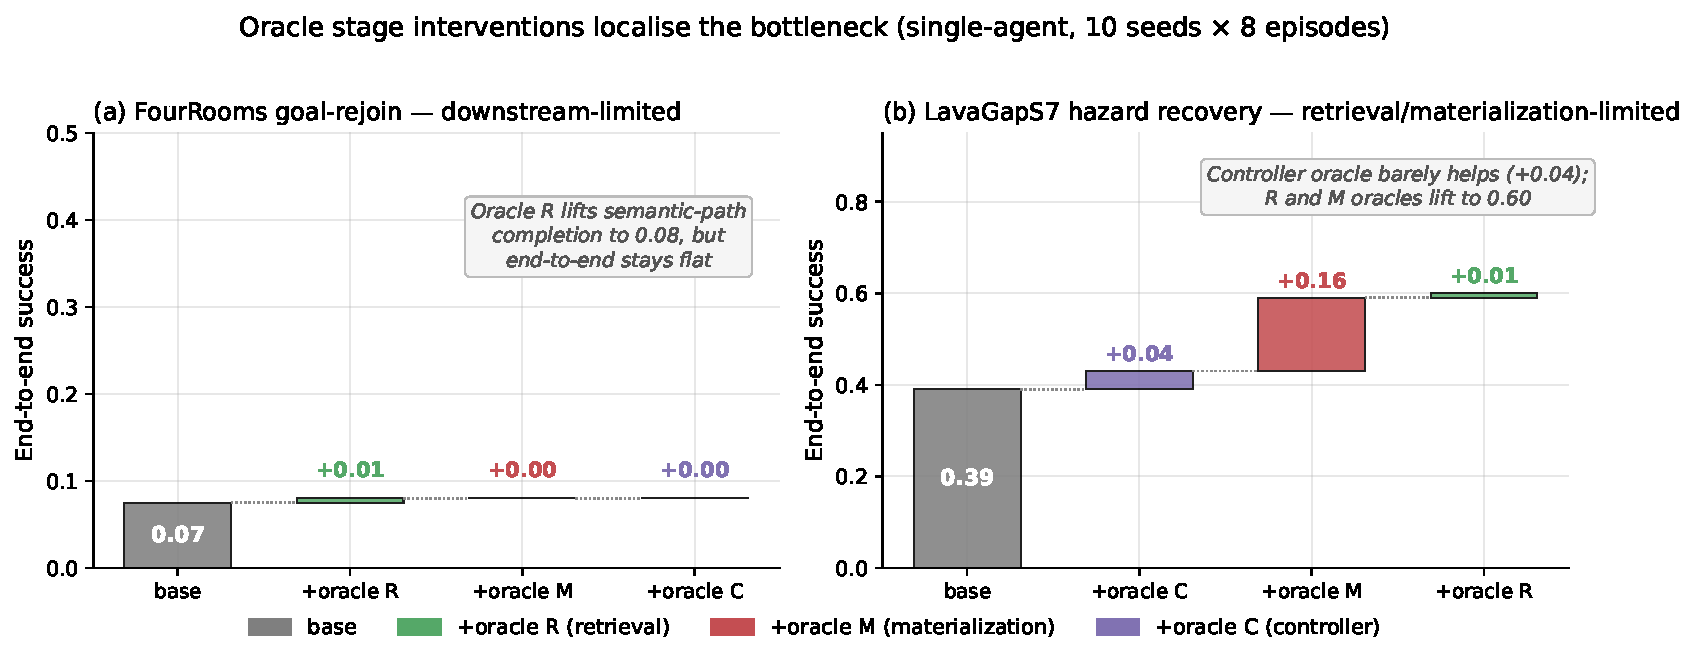
\includegraphics[width=\linewidth]{figures/fig_oracle_waterfall.pdf}
  \caption{Оракульные постадийные интервенции на двух самых трудных одноагентных семействах задач (10 сидов $\times$ 8 эпизодов). \textbf{(a)}~Возврат к цели в FourRooms: замена любой одной стадии оракулом оставляет сквозной успех на $0.07$; бутылочное горлышко --- ниже по потоку от стадий цепочки. \textbf{(b)}~Восстановление после опасности в LavaGapS7: оракульный контроллер добавляет лишь $+0.04$, но оракульная материализация добавляет $+0.16$, а оракульное извлечение --- ещё $+0.01$ до $0.60$. Фреймворк локализует стадию бутылочного горлышка постадийно.}
  \label{fig:oracle-waterfall}
\end{figure}
\FloatBarrier

\section{Переносимость и масштабирование}
\label{app:babyai}

\subsection{Перенос переносимости на BabyAI (10 сидов, полный бенчмарк)}
\label{app:babyai-deeper}

10-сидовый бенчмарк переносимости на \texttt{BabyAI-GoToObjMaze-v0}~\citep{chevalier2018babyai} (8 эпизодов на сид, max-steps 200) измерил все четыре одноагентных метода, используемых в основном бенчмарке (random, greedy, \texttt{babyai\_semantic\_node\_v1}, \texttt{babyai\_semantic\_plan\_v1}), с тем же логгером Q/R/M/C, применённым к трассам BabyAI. Числа в Таблице~\ref{tab:babyai-deeper} подтверждают, что (a) события Q/R/M/C нетривиально эмитируются на субстрате BabyAI, (b) два семантических варианта обнажают постадийно разделимую структуру там, где несемантические бейзлайны имеют $Q^\star{=}R^\star{=}M^\star{=}0$ (семантические запросы не выпускаются), и (c) упорядочение постадийных частот совпадает с бенчмарком MiniGrid (Таблица~\ref{tab:consistency}) в пределах бутстреп-ДИ. GoToObjMaze --- более трудный задачный субстрат, чем бенчмарк LavaGapS7/FourRooms из основного текста --- сквозной успех упирается в 0.15 у всех методов, --- что делает постадийную декомпозицию особенно информативной: семантический стек не выигрывает по успеху, но является единственным семейством методов, порождающим измеримые постадийные события.

\begin{table}[h]
\centering
\caption{Бенчмарк переносимости BabyAI: 10 сидов $\times$ 8 эпизодов на \texttt{BabyAI-GoToObjMaze-v0}, max-steps 200. Варианты семантического стека успешны с той же сквозной частотой, что и жадный бейзлайн (0.15), но являются единственными методами, порождающими ненулевые события Q/R/M/C --- протокол фреймворка переносится на субстрат BabyAI без модификаций. Операциональные частоты Q/R/M/C здесь оцениваются на одном и том же знаменателе (числе точек принятия решений), поэтому $Q{=}R{=}M$ у обоих семантических вариантов, поскольку GoToObjMaze эмитирует один семантический тип цели на эпизод.}
\label{tab:babyai-deeper}
\small
\begin{tabular}{l c c c c c c}
\toprule
Метод & Успех & Шаги & $Q$ (оп.) & $R$ (оп.) & $M$ (оп.) & Пост (оп.) \\
\midrule
random         & 0.125 $\pm$ 0.06 & 182.7 & 0.000 & 0.000 & 0.000 & 0.000 \\
greedy         & 0.150 $\pm$ 0.05 & 171.3 & 0.000 & 0.000 & 0.000 & 0.000 \\
semantic node  & 0.150 $\pm$ 0.05 & 171.3 & 0.032 & 0.032 & 0.032 & 0.025 \\
semantic plan  & 0.150 $\pm$ 0.05 & 171.3 & 0.032 & 0.032 & 0.032 & 0.025 \\
\bottomrule
\end{tabular}
\end{table}

\textbf{Вывод.} На второй субстрат переносится измерительный протокол фреймворка --- а не его результаты для конкретных задач. Сквозной успех на BabyAI доминируется существенно более низким потолком поэпизодного успеха GoToObjMaze, а не постадийной структурой; и наоборот, постадийная структура, которую обнажает семантический стек, идентична по форме той, что тот же стек обнажает на MiniGrid. Это ровно то свойство субстратной независимости, которое методология и призвана обеспечить. Сырые данные: \texttt{tmp/babyai\_deeper\_10seed/}.

\subsection{Многоагентное масштабирование при $N=12$}
\label{app:scale-N12}

Чтобы проверить, что многоагентные результаты \S\ref{sec:multi-agent-results} --- не артефакт диапазона $N\!\le\!8$, был выполнен дополнительный свип из 8{,}640 прогонов при $N\!=\!12$, $T \in \{6, 8, 10\}$, тех же трёх раскладках, трёх плотностях опасностей, восьми пировых каденциях и 40 сидах. Настенное время $\approx 12$ минут на 8 ядрах. Сигнатура условных частот из \S\ref{sec:multi-agent-results} сохраняется и усиливается (Таблица~\ref{tab:scale-n12}).

\begin{figure}[h]
\centering
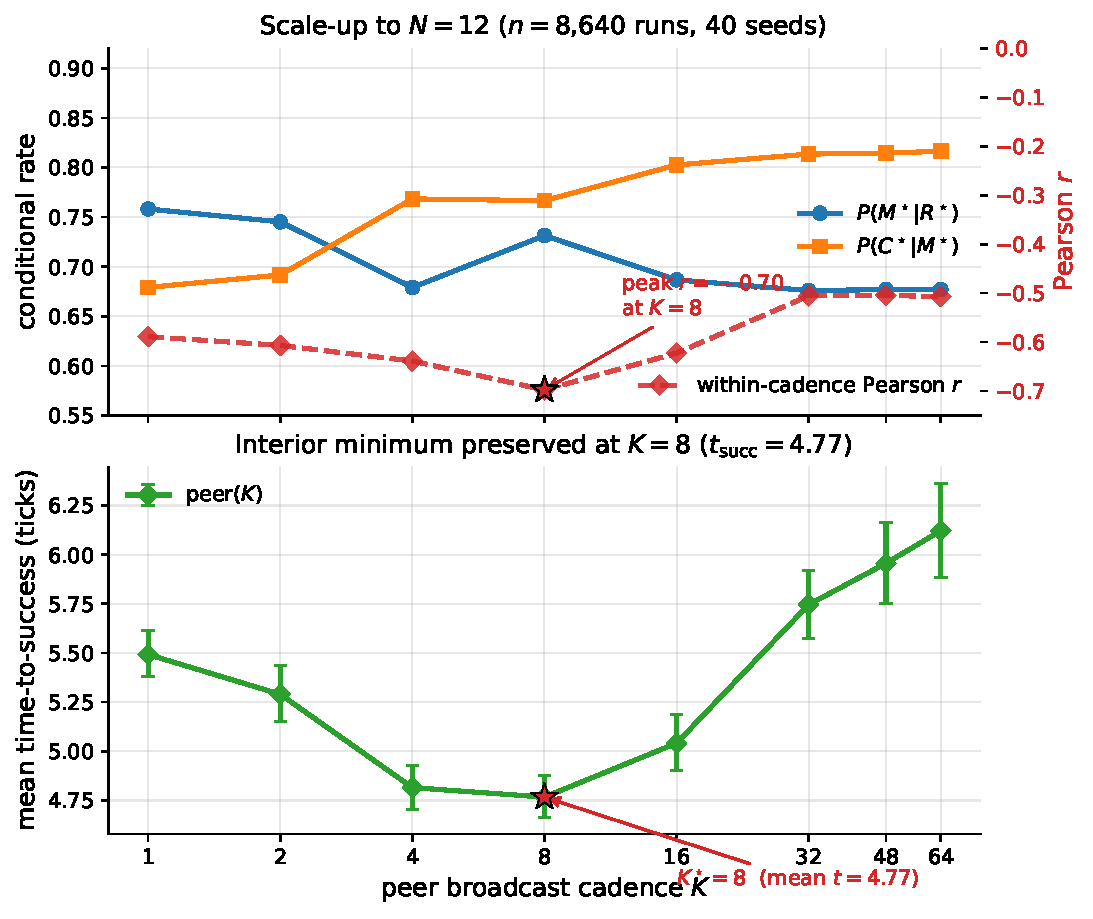
\includegraphics[width=0.92\linewidth]{figures/fig_scale_n12.pdf}
\caption{Сигнатура бутылочного горлышка при масштабировании $N\!=\!12$ ($n\!=\!8{,}640$ прогонов, 40 сидов). Сверху: покаденционные средние частоты движутся в предсказанных направлениях по $K$; внутрикаденционная корреляция Пирсона (красный пунктир, правая ось) достигает пика $-0.70$ при $K\!=\!8$ (именно этот внутрикаденционный пик и заостряется при $N{=}12$; сам M-наклон по $K$ не является кластерно-робастным при этом числе агентов, Таблица~\ref{tab:scale-n12}). Снизу: среднее время до успеха сохраняет внутренний минимум при $K\!=\!8$ ($4.77$ тиков); как и на основном свипе, положение устойчиво, но запас мелок --- зазор до соседнего $K\!=\!4$ ($4.82$ тиков) составляет $\approx0.05$ тика и не разрешён при этом размере выборки. Пик смещения бутылочного горлышка мигрирует наружу с $K\!=\!4$ при $N\!\le\!8$ до $K\!=\!8$ при $N\!=\!12$, что согласуется с тем, что более сильное связывание занятости при большем числе агентов задерживает переход между режимами издержек.}
\label{fig:scale-n12}
\end{figure}

\begin{table}[h]
\caption{Числовая детализация свипа масштабирования $N\!=\!12$ (пировая архитектура; $27$ конфигурационных ячеек). Размеры эффекта с кластерно-робастными 95\%-ми ДИ (блочный бутстреп по ячейкам): Спирмен $P(C^\star|M^\star)$ с $K$ равен $+0.31$ (ДИ $[+0.21,+0.41]$, исключает ноль), тогда как Спирмен $P(M^\star|R^\star)$ с $K$ --- лишь $-0.14$ (ДИ $[-0.28,+0.02]$, \emph{не} отделён от нуля при $N{=}12$). C-наклон Эмпирического утверждения~1 выполняется; M-наклон направленно согласован, но не кластерно-робастен при этом числе агентов. При $N{=}12$ заостряются внутрикаденционная корреляция и минимум $t_{\mathrm{succ}}$ (Рисунок~\ref{fig:scale-n12}), а не M-наклон по $K$.}
\label{tab:scale-n12}
\centering
\small
\begin{tabular}{c c c c c c}
\toprule
$K$ & $P(M^\star|R^\star)$ & $P(C^\star|M^\star)$ & MOP & среднее $t_{\mathrm{succ}}$ & корр \\
\midrule
1  & 0.758 & 0.679 & 0.475 & 5.49 & $-0.59$ \\
2  & 0.745 & 0.692 & 0.474 & 5.29 & $-0.61$ \\
4  & 0.679 & 0.768 & 0.482 & 4.82 & $-0.64$ \\
8  & 0.731 & 0.767 & 0.539 & \textbf{4.77} & $\mathbf{-0.70}$ \\
16 & 0.687 & 0.803 & 0.538 & 5.04 & $-0.62$ \\
32 & 0.676 & 0.814 & 0.538 & 5.75 & $-0.51$ \\
48 & 0.677 & 0.814 & 0.539 & 5.96 & $-0.51$ \\
64 & 0.677 & 0.816 & 0.541 & 6.12 & $-0.51$ \\
\bottomrule
\end{tabular}
\end{table}

\subsection{Q/R/M/C при семантическом, безрамочном сопоставлении мест}
\label{app:semantic-matching}

Основной свип разрешает идентичность мест общими ключами $(x,y)$. Чтобы проверить, что
декомпозиция не привязана к общему координатному субстрату, мы перезапускаем
многоагентный навигационный цикл, в котором каждый агент держит \emph{приватную}
систему координат (секретную поагентную трансляцию), а места сопоставляются
\emph{по смыслу}: локальные созвездия семантических отпечатков восстанавливают
межагентную систему координат и переносят пировые свидетельства о цели в систему координат
получателя (\method{experiments/warp/semantic\_peer\_memory.py}; раннер
\method{experiments/warp/exp\_semantic\_cadence\_qrmc.py}). Агенты навигируют
тем же планировщиком на правилах к перенесённой цели; Q/R/M/C логируются
без изменений, где $M^\star$ --- фиксация кандидата в пределах $\epsilon$ от истинной
цели ($N{=}6$, $T{=}2$ дефицитных источника воды, $8$ сидов).

Стадийные события остаются корректно определёнными без общей системы координат, и фреймворк
локализует отказ координатного предположения. \emph{Семантическое} плечо фиксирует
\emph{истинную} цель при первой материализации в $100\%$ агенто-эпизодов (при
каждой каденции); \emph{координатное} плечо --- читающее приватные
координаты пира за чистую монету --- впервые фиксирует истинную цель лишь в $25$--$52\%$
случаев (доля растёт с $K$ по мере накопления агентами собственных наблюдений), т.е.\ оно
\emph{отказывает в открытую}, материализуя фантомные клетки, не являющиеся водой. Сквозной
успех ограничен дефицитом и сопоставим между плечами ($\approx0.29\!\approx\!T/N$),
как и ожидалось. Это и есть интересующее диагностическое свойство: $M^\star$ при
координатной идентичности срабатывает на не-целях, и постадийный логгер это обнажает.

Мы \emph{не} заявляем здесь каденционного сдвига M$\leftrightarrow$C: при
рассылке все-всем и горизонте в $140$ тиков семантическая система координат восстанавливается при
каждом проверенном $K$, так что $P(M^\star|R^\star)$ каденционно-инвариантно в этой постановке
($1.00$ всюду). Эксперимент изолирует вопрос \emph{субстрата идентичности мест}:
Q/R/M/C независим от архитектуры и координат и обнаруживает
материализацию с отказом в открытую, --- а не каденционный результат, который стоит на
основном координатно-ключевом свипе. Встраивание семантического сопоставления в режим
дефицита, порождающий сдвиг, --- естественная следующая интеграция.

\section{Расширенная диагностика}
\label{app:diagnostics}

\subsection{Детализация условного произведения и разрыв Йенсена}
\label{app:phi-detail}

\begin{table*}[h]
\caption{Поархитектурные условные частоты Q/R/M/C из свипа в 35{,}640 прогонов (40 сидов). $P(R^\star|Q^\star)$ насыщено. POM = произведение средних; MOP = среднее произведений (правильное поконфигурационное ожидаемое произведение). Две сводки систематически расходятся при малых/промежуточных $K$, потому что внутрикаденционная корреляция между $P(M^\star|R^\star)$ и $P(C^\star|M^\star)$ там сильно отрицательна (последний столбец) --- сигнатура смещения бутылочного горлышка. \textbf{Жирным}: лучший по MOP среди пировых каденций. Среднее $t_{\mathrm{succ}}$ (последний столбец) --- практически значимая мера эффективности; её внутренний минимум при $K=8$ --- результат предсказанной формы, устойчивый по положению, но мелкий по запасу (соседние быстрые каденции не разрешены; Приложение~\ref{app:effect-sizes}).}
\label{tab:multi-agent-cond}
\centering
\scriptsize
\setlength{\tabcolsep}{3.5pt}
\begin{tabular}{l c c c c c c c}
\toprule
Архитектура & $P(R^\star|Q^\star)$ & $P(M^\star|R^\star)$ & $P(C^\star|M^\star)$ & POM & MOP (95\% ДИ) & корр & среднее $t_{\mathrm{succ}}$ \\
\midrule
независимая          & 0.99 & 0.68 & 0.88 & 0.598 & 0.605 [0.597, 0.614] & $+0.00$ & 8.02 \\
общая шина           & 1.00 & 1.00 & 0.60 & 0.600 & 0.595 [0.586, 0.604] & $-0.10$ & 8.33 \\
центральный агрегатор   & 1.00 & 0.97 & 0.61 & 0.592 & 0.572 [0.564, 0.580] & $-0.48$ & 7.64 \\
peer ($K=1$)         & 1.00 & 0.97 & 0.60 & 0.585 & 0.573 [0.564, 0.581] & $-0.43$ & 7.80 \\
peer ($K=2$)         & 1.00 & 0.97 & 0.62 & 0.594 & 0.576 [0.568, 0.584] & $-0.54$ & 7.59 \\
peer ($K=4$)         & 1.00 & 0.92 & 0.66 & 0.599 & 0.569 [0.561, 0.577] & $-0.61$ & 8.00 \\
peer ($K=8$)         & 0.99 & 0.69 & 0.87 & 0.597 & 0.586 [0.578, 0.595] & $-0.19$ & \textbf{7.47} \\
peer ($K=16$)        & 0.99 & 0.67 & 0.89 & 0.592 & 0.590 [0.581, 0.598] & $-0.05$ & 7.87 \\
peer ($K=32$)        & 0.99 & 0.67 & 0.89 & 0.595 & 0.598 [0.589, 0.606] & $-0.04$ & 8.28 \\
peer ($K=48$)        & 0.99 & 0.68 & 0.88 & 0.598 & 0.602 [0.593, 0.611] & $-0.02$ & 8.79 \\
peer ($K=64$)        & 0.99 & 0.68 & 0.88 & 0.599 & \textbf{0.603} [0.594, 0.611] & $-0.02$ & 9.19 \\
\bottomrule
\end{tabular}
\end{table*}

Условное произведение $\Phi = P(M^\star|R^\star)\!\cdot\!P(C^\star|M^\star)$ на свипе в 35{,}640 прогонов монотонно растёт по $K$ на $K\in\{4,8,16,32,48,64\}$ и сходится к границе независимых агентов $\Phi(K\!\to\!\infty)=0.605$. Парный бутстреп: $\Delta(K{=}32{-}K{=}16) = +0.008$ (ДИ $[+0.006, +0.010]$), $\Delta(K{=}48{-}K{=}16) = +0.011$, $\Delta(K{=}64{-}K{=}16) = +0.012$; уровень независимых агентов лежит выше каждого пирового $K$, кроме $K\!=\!64$ (где ДИ зазора включает ноль). Это утверждение об \emph{уровне} $\Phi$ на проверенных каденциях, а не о \emph{форме} $\Phi(K)$: согласуясь с монотонным трендом, мы не заявляем внутреннего экстремума (\S\ref{sec:shift}).

Отрицательная внутрикаденционная ковариация, задокументированная в \S\ref{sec:multi-agent-results}, создаёт разрыв неравенства Йенсена между $\Phi$ и маргинальным произведением средних: $E[X]\!\cdot\!E[Y] > E[X\!\cdot\!Y]$ при $\mathrm{Cov}(X,Y) < 0$. Среднее произведений сообщается как первичная сводка, потому что оно корректно впитывает ковариацию. Рисунок~\ref{fig:bottleneck-shift} показывает K-свиповый вид обеих условных частот и среднего $t_{\mathrm{succ}}$; Рисунок~\ref{fig:jensen-scatter} показывает поконфигурационный скаттер, который суммирует отрицательная ковариация.

\begin{figure}[t]
  \centering
  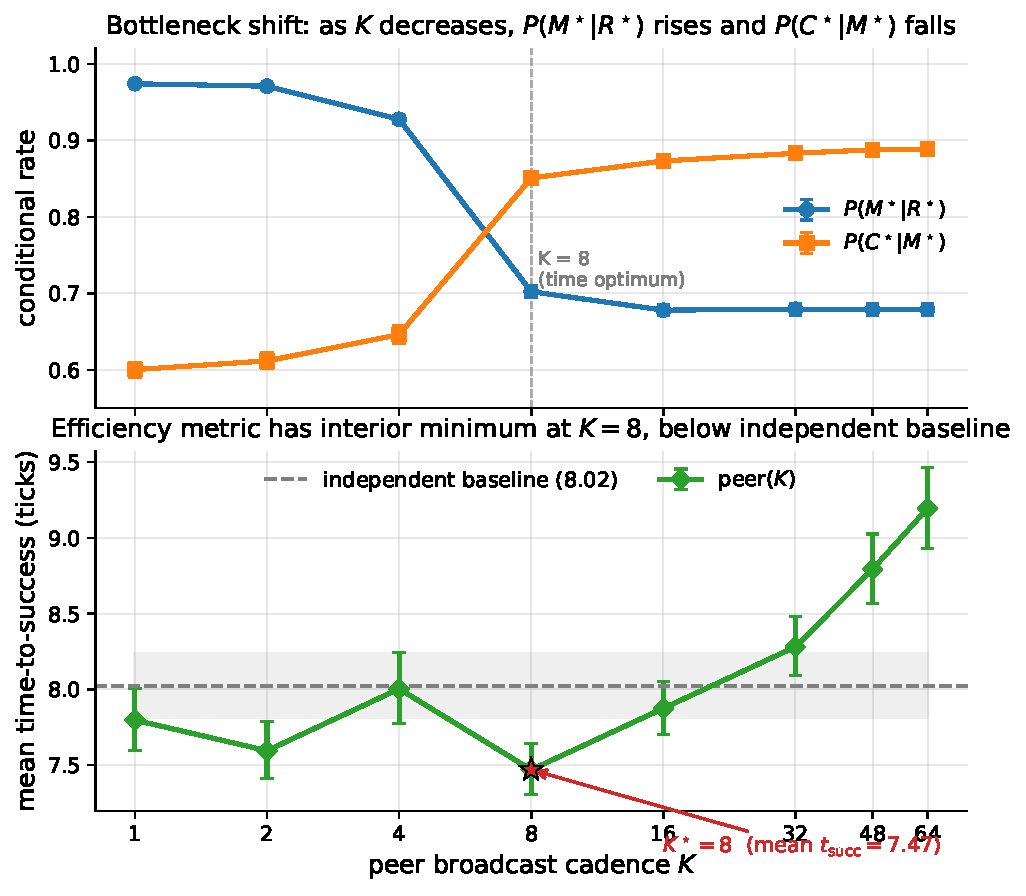
\includegraphics[width=0.85\linewidth]{figures/fig_bottleneck_shift.pdf}
  \caption{Смещение бутылочного горлышка по восьми пировым каденциям (40-сидовый свип). Сверху: $P(M^\star|R^\star)$ падает, а $P(C^\star|M^\star)$ растёт по $K$ (умеренные, кластерно-робастные спирменовские размеры эффекта $-0.53$ и $+0.43$; ДИ в Приложении~\ref{app:effect-sizes}). Снизу: среднее время до успеха имеет внутренний минимум при $K=8$ ($7.47$ тиков) ниже бейзлайна независимых агентов ($8.02$, пунктир); положение устойчиво, но его запас над соседними быстрыми каденциями ($K{=}1,4$) не разрешён (Приложение~\ref{app:effect-sizes}). Планки погрешностей и затенённая полоса --- 95\%-е бутстреп-ДИ.}
  \label{fig:bottleneck-shift}
\end{figure}

\begin{figure}[t]
  \centering
  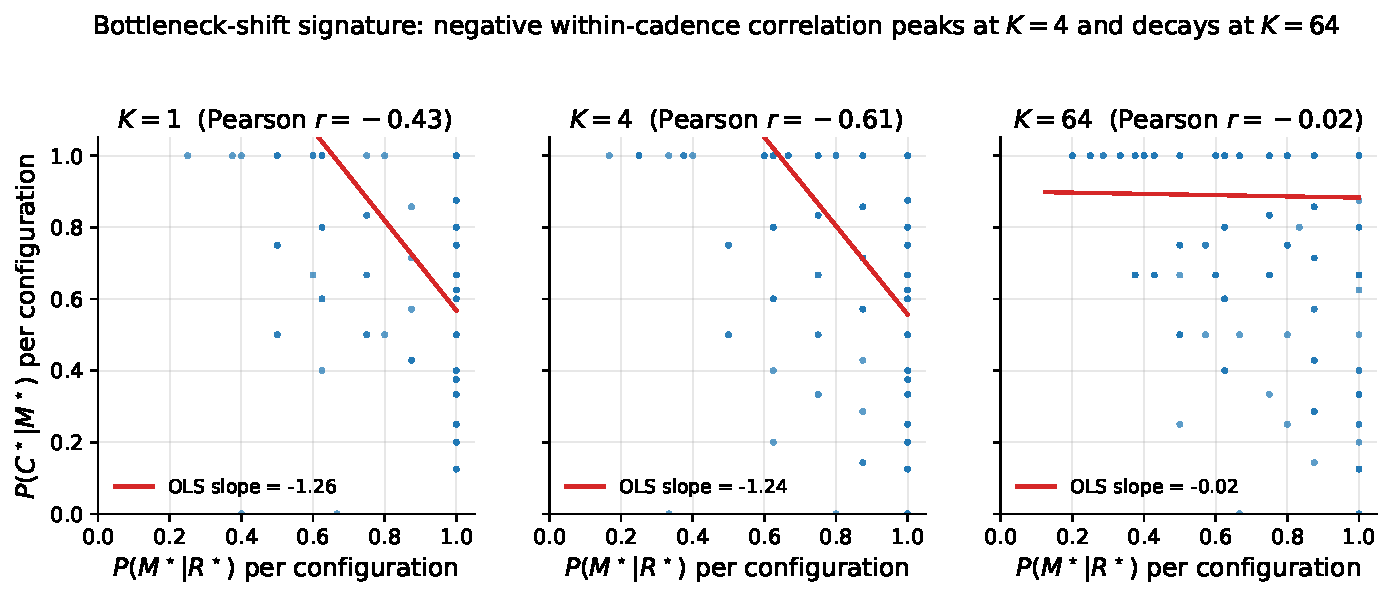
\includegraphics[width=0.95\linewidth]{figures/fig_jensen_scatter.pdf}
  \caption{Поконфигурационный скаттер $P(M^\star|R^\star)$ против $P(C^\star|M^\star)$ при трёх каденциях. Сильная отрицательная корреляция при $K=4$ (Пирсон $-0.61$) --- сигнатура смещения бутылочного горлышка: те же конфигурации, что успешны на $M$, склонны отказывать на $C$, и наоборот. Корреляция затухает до шума к $K=64$.}
  \label{fig:jensen-scatter}
\end{figure}

\subsection{Декомпозиция дизайна и сверка числа прогонов}
\label{app:design}

Число $35{,}640$ раскладывается в точности как в Таблице~\ref{tab:design}. Базовый дизайн --- девять допустимых дефицитных пар $(N,T)$ (для $N{=}3$: $T{\in}\{2,3\}$; $N{=}5$: $T{\in}\{2,3,5\}$; $N{=}8$: $T{\in}\{2,3,5,8\}$), скрещённых с тремя раскладками, тремя плотностями опасностей и 40 сидами, что даёт $3{,}240$ базовых конфигураций. Пировая архитектура прогоняется на всех восьми каденциях ($3{,}240\times 8 = 25{,}920$); три бескаденционные архитектуры (независимая, общая шина, центральный агрегатор) вносят по $3{,}240$ каждая. Число $25{,}920$ прогонов, используемое для пирового кластерно-робастного анализа (Приложение~\ref{app:effect-sizes}), --- это в точности пировый блок; первоначальный разведочный свип из $12{,}960$ прогонов (\S\ref{sec:shift}, «Хронология») и свипы расширенных каденций и $N{=}12$ (Приложение~\ref{app:babyai}) --- отдельные наборы прогонов и не смешиваются с основным свипом.

\begin{table}[h]
\caption{Сверка числа прогонов для основного многоагентного свипа ($35{,}640$ прогонов). Счётчики пересчитаны напрямую из опубликованного лога прогонов.}
\label{tab:design}
\centering
\small
\begin{tabular}{l l r}
\toprule
Фактор & Уровни & Число \\
\midrule
Дефицитные пары $(N,T)$ & $(3,2)(3,3)(5,2)(5,3)(5,5)(8,2)(8,3)(8,5)(8,8)$ & 9 \\
Раскладки & симметричная, асимметричная, случайная & 3 \\
Плотности опасностей & $0.0,\ 0.05,\ 0.10$ & 3 \\
Сиды & & 40 \\
\midrule
Базовые конфигурации & $9\times3\times3\times40$ & 3{,}240 \\
Peer (все 8 каденций $K$) & $3{,}240\times8$ & 25{,}920 \\
Независимая / шина / центральная & $3\times3{,}240$ & 9{,}720 \\
\midrule
\textbf{Итого} & & \textbf{35{,}640} \\
\bottomrule
\end{tabular}
\end{table}

\subsection{Размеры эффекта и кластерно-робастный вывод}
\label{app:effect-sizes}

Величины $p<10^{-4}$, приведённые в \S\ref{sec:multi-agent-results}, сообщаются для полноты, но не являются основанием утверждения: на десятках тысяч прогонов почти любой ненулевой наклон «значим», а прогоны не независимы --- они кластеризуются внутри конфигурации $(N,T,\text{раскладка},\text{опасность})$. Полный свип содержит $25{,}920$ пировых прогонов, но лишь \textbf{81 независимую ячейку дизайна}. Поэтому мы сообщаем размеры эффекта с кластерно-робастными доверительными интервалами из блочного бутстрепа, ресемплирующего \emph{конфигурационные ячейки} (а не строки), $B{=}4000$ ресемплов.

Два наклона Эмпирического утверждения~1 выживают как подлинные, но умеренные эффекты: спирменовская корреляция $P(M^\star|R^\star)$ с $K$ равна $\rho=-0.53$ (95\%-й кластерный ДИ $[-0.59,-0.47]$, сильная), а $P(C^\star|M^\star)$ с $K$ --- $\rho=+0.43$ (95\%-й кластерный ДИ $[+0.37,+0.50]$, умеренная). Оба интервала исключают ноль при ресемплировании на уровне ячеек, так что смещение бутылочного горлышка --- не артефакт коррелированного числа прогонов; это умеренный монотонный тренд, и мы описываем его именно так, а не как почти детерминированный закон.

Внутренний оптимум на среднем времени до успеха устойчив по \emph{положению}, но мелок по \emph{запасу}. Парный блочный бутстреп на ячеечных разностях $t_{\mathrm{succ}}$ даёт $t_{\mathrm{succ}}(K{=}8)$ ниже $t_{\mathrm{succ}}(K{=}16)$ на $0.40$ тика (ДИ $[0.08,0.83]$) и ниже $K{=}64$ на $1.67$ тика (ДИ $[0.75,2.83]$), оба разрешены; но его преимущество над $K{=}4$ ($0.49$, ДИ $[-0.47,1.51]$) и $K{=}1$ ($0.27$, ДИ $[-0.43,0.97]$) --- в пределах шума.\footnote{Этот парный бутстреп и спирменовские корреляции размеров эффекта выше вычислены на том же исполнении свипа, что и Таблица~\ref{tab:multi-agent-cond} ($25{,}920$ пировых прогонов); статистика $t_{\mathrm{succ}}$ определена только на успешных эпизодах, так что парная ячеечная разность ($1.67$ для $K{=}8$ против $K{=}64$) относится к этой субпопуляции и совпадает с разностью маргинальных средних в Таблице~\ref{tab:multi-agent-cond} ($9.19{-}7.47{=}1.72$) с точностью до округления. Размеры эффекта идентичны на независимом исполнении \texttt{paper1\_clean} ($-0.531$/$+0.434$), что подтверждает их непривязанность к конкретному прогону.} Взвешенная успехом метрика эффективности ($t_{\mathrm{succ}}$, делённое на долю успеха) имеет тот же внутренний $\arg\min$ при $K{=}8$, так что положение оптимума устойчиво к определению эффективности, даже если его запас над соседними быстрыми каденциями не разрешён при этом размере выборки. Мы читаем это как поддержку \emph{формы}, предсказанной компромиссом M$\leftrightarrow$C, а не остро настроенной оптимальной каденции.

\subsection{Конструктная валидность: успех задачи $Y$ против завершения семантического пути $C^\star$}
\label{app:y-vs-c}

Успех $Y$ в принципе может обойти семантический путь, так что постадийное бутылочное горлышко в $Q/R/M/C$ не обязано объяснять вариацию $Y$. Два факта ограничивают это опасение. Во-первых, в многоагентном свипе, о котором Эмпирическое утверждение~1, успех \emph{определяется} как достижение цели \texttt{water\_source}, что и есть в точности событие $C^\star$; эмпирически $Y$ и $C^\star$ совпадают прогон в прогон (корреляция $1.00$, средний зазор $0.00$). Центральное многоагентное утверждение тем самым не уязвимо для возражения о параллельном канале. Во-вторых, зазор $Y>C^\star$ --- одноагентный феномен на лёгких семействах задач (вода, отдых), где запасной контроллер может достичь цели без семантической фиксации цели; он наибольший ровно там, где успех уже высок и диагноз наименее нужен, и исчезает на трудных семействах (восстановление после опасности, целевой регион), где фреймворк и делает свою работу. Поэпизодная, постадийно разрешённая медиация $Y$ (а не $C^\star$) требует логов, помечающих каждый успех тем, прошёл ли он семантический путь, и является планируемым уточнением инструментирования.

\subsection{Робастность диагноза пустого множества кандидатов к порогу ($\theta$)}
\label{app:theta-robustness}

Одноагентная атрибуция «отказывает генерация кандидатов, не ранжирование»
(\S\ref{sec:refined-attribution}) опирается на высокую долю пустых множеств кандидатов.
Рецензент спрашивает, не артефакт ли это порога обязательных тегов
$\theta$ (развёрнутое значение $0.5$; гейт кандидатства ---
$\mathrm{profile}[\text{tag}]\ge\theta$ в
\method{symbolic\_memory.\_required\_matches\_profile}). Мы свипуем $\theta$ через
переопределение в построителе запросов (\method{experiments/big\_experiment/theta\_ablation.py});
крайние точки подтверждают, что гейт работает, а рабочий диапазон показывает, что
диагноз --- не пороговый эффект.

\begin{table}[h]
\caption{Доля пустых множеств кандидатов против порога обязательных тегов $\theta$ (семантический метод, ассист выкл., восстановление после опасности / целевой регион). Доля \emph{инвариантна} по всему реалистичному диапазону $\theta\in[0.05,0.95]$; лишь вырожденные крайние точки её сдвигают, и лишь до пола отсутствия кандидатов. Пустоты, следовательно, --- отсутствие сохранённых свидетельств, а не подпороговая фильтрация.}
\label{tab:theta-robustness}
\centering
\small
\begin{tabular}{c c c}
\toprule
$\theta$ & доля пустых (восст. после опасности) & доля пустых (целевой регион) \\
\midrule
$0.00$ (принять всё) & 0.50 & --- \\
$0.05$ & 0.533 & 0.267 \\
$0.15$ & 0.533 & 0.267 \\
$0.25$ & 0.533 & 0.267 \\
$0.50$ (развёрнутый) & 0.533 & 0.267 \\
$0.75$ & 0.533 & 0.267 \\
$0.95$ & 0.533 & 0.267 \\
$1.00$ (не принимать ничего) & 0.75 & --- \\
\bottomrule
\end{tabular}
\end{table}

Прочтение решающее (Таблица~\ref{tab:theta-robustness}). При $\theta{=}1.0$ ничего не проходит, и доля пустых растёт; при $\theta{=}0.0$ гейт обязательных тегов принимает каждый узел ($\mathrm{conf}\ge 0$ выполняется всегда), однако доля пустых падает лишь до $0.50$ --- своего пола, --- то есть в этих точках принятия решений \emph{нет узла-кандидата какой бы то ни было уверенности} для извлечения. По всему разумному диапазону $\theta\in[0.05,0.95]$ доля плоская на $0.533$: ослабление или ужесточение порога не возвращает кандидата, потому что требуемое семантическое место никогда не было сохранено. Это в точности режим «отсутствие свидетельств, а не противоречие», названный в \S\ref{sec:event-semantics}, теперь показанный порогово-инвариантным, так что атрибуция накопления памяти --- не артефакт $\theta$. (Абсолютные доли здесь --- на малом свипе восстановления после опасности / целевого региона и не являются заголовочными $91\%$ из \S\ref{sec:refined-attribution}, которые относятся к полному бенчмарку; суть в $\theta$-инвариантности, а не в уровне.)

\subsection{Робастность к нарушениям Предположения~1}
\label{app:assumption1-stress}

Определение~1 покоится на условном постадийно-марковском свойстве (Предположение~1). Два практически значимых нарушения --- адаптивные переписывания запроса, не всплывающие в логгер, и скрытые межстадийные обновления памяти --- ровно те случаи, когда \emph{нелогируемая латентная} переменная связывает несмежные стадии. Мы количественно оцениваем результирующее смещение оценки контролируемой симуляцией ($4\!\times\!10^5$ эпизодов на настройку; \method{experiments/big\_experiment/assumption1\_stress\_test.py}). Эпизоды генерируются с известными механизменными частотами $P(M^\star|R^\star){=}0.70$, $P(C^\star|M^\star){=}0.65$ и скрытой бинарной латентной $U$, сдвигающей \emph{обе} частоты M и C на $\pm\delta$; наивная оценка обусловливается лишь предыдущей звёздной стадией, не $U$.

\begin{table}[h]
\caption{Смещение наивных условных оценок при нелогируемой латентной силы $\delta$, связывающей стадии M и C (нарушая Предположение~1). $P(M^\star|R^\star)$ остаётся несмещённым; $P(C^\star|M^\star)$ смещено вверх, существенно лишь при сильном связывании.}
\label{tab:assumption1-stress}
\centering
\small
\begin{tabular}{c c c}
\toprule
$\delta$ (сила связывания) & смещение $\hat P(M^\star|R^\star)$ & смещение $\hat P(C^\star|M^\star)$ \\
\midrule
0.00 & $-0.001$ & $-0.002$ \\
0.05 & $+0.001$ & $+0.004$ \\
0.10 & $+0.001$ & $+0.015$ \\
0.15 & $-0.000$ & $+0.031$ \\
0.20 & $+0.000$ & $+0.056$ \\
0.25 & $-0.001$ & $+0.089$ \\
\bottomrule
\end{tabular}
\end{table}

Два вывода (Таблица~\ref{tab:assumption1-stress}). Условная вероятность R$\to$M несмещена при каждом $\delta$: латентная переменная перевзвешивает эпизоды, но не конфаундит это ребро. Условная вероятность C$\to$M приобретает однознаковое смещение \emph{вверх} --- латентная делает эпизоды с высоким M также эпизодами с высоким C, так что обусловливание на M пересчитывает завершение, --- но смещение составляет лишь $+1.5$ процентного пункта при мягком нарушении ($\delta\!\le\!0.10$) и достигает $+5.6$ пункта лишь при сильном нелогируемом связывании ($\delta{=}0.20$). Уязвимость фреймворка к нарушениям Предположения~1, следовательно, ограничена, и направление его отказа известно --- что и есть релевантное утверждение о робастности для применения логгера к обученным или LLM-агентам, где такие связывания более обычны.

\subsection{Предварительная проверка на непрерывном субстрате (VMAS)}
\label{app:vmas}

Самая запрашиваемая проверка робастности --- специфично ли смещение бутылочного горлышка
M$\leftrightarrow$C для сеточных субстратов. Мы сообщаем \emph{предварительный}
положительный результат на субстрате с непрерывным пространством состояний (VMAS~\citep{bettini2022vmas}).
Символьная пировая память и операциональные определения Q/R/M/C переиспользуются
без изменений; тонкий мост дискретизации отображает непрерывные $(x,y)$ в грубые клетки,
чтобы память была применима, а контроллер действует в непрерывном пространстве к
материализованной путевой точке (\method{experiments/vmas\_portability/}). Материализация
использует ту же чувствительную к занятости фиксацию, что и сеточный планировщик (кандидат, чья
цель уже заявлена, не фиксируется).

\begin{table}[h]
\caption{Предварительная переносимость VMAS: оба знака наклонов Эмпирического утверждения~1 воспроизводятся на непрерывном субстрате в режиме связывания ($N{=}8$, $T{=}3$, 40 сидов, горизонт $25$). $\mathrm{Spearman}(P(M^\star|R^\star),K){=}-1.00$ и $\mathrm{Spearman}(P(C^\star|M^\star),K){=}+1.00$. За пределами $K\!\approx\!32$ система входит в независимый режим (редкая рассылка, нет соперничества), и $P(M^\star|R^\star)$ отскакивает --- та же граница режимов, что видна на сетке.}
\label{tab:vmas}
\centering
\small
\begin{tabular}{c c c}
\toprule
$K$ & $P(M^\star|R^\star)$ & $P(C^\star|M^\star)$ \\
\midrule
1  & 1.000 & 0.182 \\
2  & 0.583 & 0.305 \\
4  & 0.448 & 0.405 \\
8  & 0.305 & 0.608 \\
16 & 0.278 & 0.639 \\
\bottomrule
\end{tabular}
\end{table}

Мы помечаем это как предварительное и не вливаем в заголовочные утверждения: это
одна конфигурация сценария, горизонт короток, кластерно-робастных ДИ пока нет,
память питается через мост дискретизации (непрерывная
\emph{динамика} с дискретизованной символьной \emph{памятью}, а не полностью непрерывная
память), а сообщаемый Спирмен $\pm1.00$ --- \emph{идеальная} ранговая
корреляция всего лишь по пяти монотонным точкам ($K\le16$) --- слабое свидетельство само по
себе, указывающее направление, а не разрешённый размер эффекта. Что оно устанавливает --- так это что два знака наклонов не являются артефактом
клеток сетки: тот же механизм «свежесть против соперничества» действует, когда позиции
и движение непрерывны. Повышение этого до заголовочного результата требует масштабирования
до нескольких ячеек дефицита и раскладок с кластерно-робастным бутстрепом из
Приложения~\ref{app:effect-sizes}.

\subsection{Каденционная робастность: сдвиг отслеживает дефицит, а не устройство сетки}
\label{app:cadence-robustness}

Рецензент может возразить, что смещение бутылочного горлышка встроено в сетку с дефицитными
целями и фиксациями. Если же это сигнатура соперничества за \emph{дефицитные
общие} цели, её условия на наклоны должны ломаться при изобилии целей. Мы
перезапускаем пировый каденционный свип в трёх режимах на той же среде ($N{=}8$, случайная
раскладка, опасность $0.05$, $20$ сидов; \method{experiments/big\_experiment/exp\_cadence\_robustness.py}):
дефицит ($T{=}3$), пограничный ($T{=}N{=}8$) и изобилие ($T{=}14{>}N$).

\begin{table}[h]
\caption{Два условия на наклоны Эмпирического утверждения~1 (\S\ref{sec:shift}) выполняются при дефиците и выполаживаются при изобилии. $P(M^\star|R^\star)$ должно падать, а $P(C^\star|M^\star)$ расти по $K$; «корр» --- внутрикаденционная корреляция Пирсона двух звеньев при $K{=}64$ (сигнатура сдвига). $P(C^\star|M^\star)$ --- операциональное отношение (ограничено $1$; изобилие завершает без формальной фиксации).}
\label{tab:cadence-robustness}
\centering
\small
\begin{tabular}{l c c c c}
\toprule
Режим & $P(M^\star|R^\star)$: $K{=}1\!\to\!64$ & $P(C^\star|M^\star)$: $K{=}1\!\to\!64$ & корр$(M,C)$ @ $K{=}64$ & argmin $t_{\mathrm{succ}}$ \\
\midrule
Дефицит ($T{=}3$)      & $0.86 \to 0.49$ (падает) & $0.51 \to 0.79$ (растёт) & $-0.86$ & $K{=}4$ (внутр.) \\
Пограничный ($T{=}N{=}8$) & $0.79 \to 0.72$        & $0.77 \to 0.95$ (растёт) & $-0.79$ & $K{=}8$ (внутр.) \\
Изобилие ($T{=}14$)    & $0.74 \to 0.77$ (плоско)  & $1.00 \to 0.99$ (плоско)  & $-0.29$ & $K{=}4$ \\
\bottomrule
\end{tabular}
\end{table}

Оба наклона присутствуют при дефиците, ослабевают на границе и \emph{выполаживаются}
при изобилии: при большем числе целей, чем агентов, соперничества нет, так что быстрый
обмен ни перенасыщает материализацию ($P(M^\star|R^\star)$ остаётся плоским
на $\sim0.75$ вместо всплеска с последующим падением), ни коллапсирует завершение
($P(C^\star|M^\star)$ остаётся на $\sim1$ даже при $K{=}1$ вместо падения до
$0.51$). Внутрикаденционная антикорреляция M$\leftrightarrow$C монотонно
ослабевает с изобилием ($-0.86\to-0.79\to-0.29$). Сдвиг, следовательно,
отслеживает \emph{механизм соперничества} и исчезает при его устранении --- он
не является фиксированным артефактом дизайна «сетка плюс фиксации». Честно отметим, что
внутренний оптимум $t_{\mathrm{succ}}$ более общ (присутствует во всех трёх
режимах): он отражает издержки исследования/пути очень быстрого \emph{или} очень
медленного обмена, где соперничество за цели --- один из вкладчиков, но не единственный.

\subsection{Открытые проблемы, подсказанные диагностикой}
\label{app:open-problems}

Четыре конкретных вопроса следуют напрямую из измерений \S\ref{sec:refined-attribution} и \S\ref{sec:multi-agent-results}.
\textbf{(1)~Адаптивная каденция.} Эмпирическое утверждение~1 предполагает фиксированный $K$; сигнатура смещения бутылочного горлышка подсказывает онлайн-контроллер $K_t$, рассылающий, когда (оцененный) выигрыш на стороне M превышает занятостную цену на стороне C.
\textbf{(2)~Селективная консолидация.} Обмен снимками сливает всё; правила слияния, приоритизирующие свидетельства о недопредставленных семантических тегах, атакуют голодание генерации кандидатов из \S\ref{sec:refined-attribution} напрямую.
\textbf{(3)~Слияние, взвешенное доверием, при занятости.} Центральный агрегатор уже выполняет слияние, взвешенное доверием, но платит цену C-коллапса; децентрализованные правила доверия, учитывающие \emph{намерение} пира (а не только его свидетельства), могли бы расцепить свежесть и гонку за цели. \emph{Со времени подачи первого драфта эта проблема решена конструктивно}: децентрализованный протокол, в котором фиксация цели агента подсаживает лёгкое \emph{резервирование} на его следующую запланированную рассылку (без координатора, без дополнительного канала), а фиксации, доминируемые более ранним резервированием, отзываются анти-$M^\star$ откатом с экспоненциальным бэкоффом. На ячейках дефицита это возвращает потерю завершения быстрых каденций на \emph{безусловных} метриках --- доля успеха растёт при каждом $K\in\{1,2,4\}$ с непересекающимися бутстреп-ДИ, а быстрый обмен с протоколом превышает бейзлайн оптимума $K{=}8$ ($0.614$--$0.620$ против $0.583$) --- с латентностью отката, ограниченной ${\approx}K$ тиками. Детали --- в сопутствующей рукописи; открытая проблема пересмотрена в сторону её более трудных вариантов (адаптивная область резервирования, гетерогенное доверие).
\textbf{(4)~Общность субстрата.} Декомпозиция переносится между MiniGrid, BabyAI, собственной сеткой и многоагентной обёрткой стандартного MiniGrid с идентичными операциональными определениями и подтверждёнными знаками наклонов Эмпирического утверждения~1 ($\S$~\ref{sec:limitations}), а предварительная проверка воспроизводит оба наклона на VMAS-субстрате с непрерывным пространством состояний (Приложение~\ref{app:vmas}). Декомпозиция также координатно-независима: при \emph{семантическом}, безрамочном сопоставлении мест (агенты в приватных системах координат, места сопоставляются по смыслу) стадийные события остаются корректно определёнными и обнажают материализацию координатного предположения с отказом в открытую (Приложение~\ref{app:semantic-matching}). Полная валидация в непрерывном пространстве состояний с кластерно-робастными ДИ и более богатые 3D-субстраты (Habitat~\citep{savva2019habitat}) остаются следующими шагами переносимости.

\subsection{Расширенный обзор литературы}
\label{app:related-work-extended}

Классические перспективы когнитивных карт мотивируют явные абстракции мест \citep{tolman1948cognitive,okeefe1978hippocampus,kuipers2000spatial}; современный воплощённый ИИ сочетает картирование и планирование \citep{gupta2017cognitive} или открывает топологическую память (SPTM, \citealp{savinov2018semi}); целеобусловленный RL обусловливается явными целями или эмбеддингами \citep{andrychowicz2017hindsight,ghosh2021learning}, а работы о репрезентации преемника дают предиктивную структуру \citep{dayan1993improving,stachenfeld2017hippocampus,momennejad2017successor}. Наша постановка отличается тем, что цель --- семантический паттерн, извлекаемый из памяти, а не координата. В многоагентном RL доминирует CTDE \citep{lowe2017maddpg,foerster2018ctde}, а обученная коммуникация добавляет пошаговую переменную обмена \citep{sukhbaatar2016commnet,foerster2016learning}; протоколы gossip и консенсуса \citep{boyd2006gossip,xiao2007distributed} --- ближайший сетевой аналог нашей оси каденции, поднятой здесь на уровень когнитивной архитектуры. Системы LLM-агентов сочетают рассуждение/действие, рефлексию, явную память и многоагентную беседу \citep{yao2022react,shinn2023reflexion,wang2023voyager,park2023generative,wu2023autogen,packer2023memgpt,chhikara2025mem0}. Наш фреймворк ортогонален: вместо обучения коммуникационной политики сквозным образом он \emph{диагностирует}, где в цепочке Q/R/M/C данная архитектура успешна или отказывает, и даёт предсказание уровня наклонов о каденции, проверяемое на логах.

\subsection{SOTA-бейзлайн и матрица покрытия}
\label{app:sota-coverage}

Таблица~\ref{tab:sota-coverage} разделяет прямые экспериментальные бейзлайны и более широкие SOTA-референсы. Локальные эксперименты намеренно скромны и полностью инструментированы: random / graph-only / SPTM-like / обученный BC в MiniGrid, CommNet PPO в многоагентной сетке и исследование бюджета шагов LLM на TextNav на двух локальных моделях Ollama (в котором Q/R/M/C локализует отказ, ограниченный завершением, \S\ref{sec:multi-agent-results}). ReAct, Reflexion, Voyager, Generative Agents, AutoGen, MemGPT и Mem0 здесь не реимплементируются как полные системы; они определяют текущее пространство дизайна агентов с памятью, относительно которого Q/R/M/C позиционируется как диагностический протокол.

\paragraph{Позиционирование относительно SOTA-дизайнов памяти.}
Пространство дизайна агентов с памятью можно организовать по двум осям: один против многих агентов, и как память представлена и разделяется (Таблица~\ref{tab:sota-quadrants}). Векторно-эмбеддинговая память (MemGPT, Voyager --- одноагентные; Generative Agents --- многоагентная) извлекает непрозрачным поиском ближайших соседей, так что отказ не локализуем по стадии. Дизайны с общим контекстом (MetaGPT, AutoGen) сваливают всё в одно окно, растворяя поагентное состояние. MARL с обученной коммуникацией (CommNet и более сильные CTDE-методы QMIX \citep{rashid2018qmix}, MAPPO \citep{yu2022mappo}, MADDPG \citep{lowe2017maddpg}) оптимизирует канал сообщений сквозным образом и, как мы верифицируем для CommNet PPO (\S\ref{sec:multi-agent-results}), не эмитирует разделимых событий запроса/фиксации/завершения. Ячейка, которую занимает наша система --- поагентная \emph{символьная} память с явным интерфейсом запроса/извлечения/материализации, обмениваемая с настраиваемой каденцией, --- в этой матрице пуста, и именно этот интерфейс делает четыре стадии Q/R/M/C наблюдаемыми. Наше утверждение против SOTA, следовательно, --- не более высокая награда, а более высокая \emph{диагностируемость при сопоставимом успехе задачи}: тот самый интерфейс, который сильный обученный метод выторговывает в пользу сквозной оптимизации, и позволяет фреймворку локализовать, где память помогает.

\begin{table}[h]
\caption{Где фреймворк сидит в пространстве дизайна агентов с памятью. Постадийная наблюдаемость Q/R/M/C требует явного интерфейса запроса/фиксации, который и предоставляет ячейка «символьная поагентная».}
\label{tab:sota-quadrants}
\centering
\small
\begin{tabular}{p{3.1cm} p{4.3cm} p{4.3cm}}
\toprule
Представление памяти & Один агент & Много агентов \\
\midrule
Векторно-эмбеддинговая память & MemGPT, Voyager \citep{packer2023memgpt,wang2023voyager} & Generative Agents \citep{park2023generative} \\
Общее контекстное окно & --- & AutoGen \citep{wu2023autogen} \\
MARL с обуч.\ коммуникацией & --- & CommNet, QMIX, MAPPO, MADDPG \citep{sukhbaatar2016commnet,rashid2018qmix,yu2022mappo,lowe2017maddpg} \\
Символьная поагентная + явный интерфейс & Q/R/M/C один агент (\S\ref{sec:single}) & \textbf{эта работа} (пировая память, каденция $K$) \\
\bottomrule
\end{tabular}
\end{table}

\begin{table*}[h]
\caption{SOTA-покрытие для Статьи 1. «Инструментировано» означает, что прогон эмитирует операциональные события $Q^\star,R^\star,M^\star,C^\star$, используемые Определением~1.}
\label{tab:sota-coverage}
\centering
\small
\begin{tabular}{p{2.45cm}p{2.55cm}p{2.7cm}p{4.0cm}}
\toprule
Семейство & Репрезентативный метод & Статус в этой статье & Точка сравнения Q/R/M/C \\
\midrule
Топологическая навигационная память & SPTM-подобный графовый бейзлайн \citep{savinov2018semi} & Прямой бейзлайн MiniGrid & Проверяет, обнажает ли топологическая память без семантического запроса/фиксации нетривиальные стадийные события. \\
Клонирование поведения & Обученный BC на сеточных наблюдениях & Прямой бейзлайн MiniGrid & Сильный успех на лёгких задачах, но без явного интерфейса запроса/фиксации, так что диагностика структурно ограничена. \\
Обученная коммуникация & CommNet PPO \citep{sukhbaatar2016commnet,schulman2017proximal} & Прямой многоагентный бейзлайн & Конкурентоспособный успех; $Q^\star$ насыщается и R/M схлопываются, верифицируя потерю наблюдаемости. \\
Кооперативный MARL (CTDE / декомпозиция ценности) & QMIX, MAPPO, MADDPG \citep{rashid2018qmix,yu2022mappo,lowe2017maddpg} & Референс первоисточников & Более сильные сквозные бейзлайны, чем CommNet; они оптимизируют совместную политику/канал сообщений без явного интерфейса запроса/фиксации, так что применим тот же аргумент о коллапсе наблюдаемости --- фреймворк квантифицирует диагностическую цену неявной координации, а не соревнуется по награде. \\
LLM-агенты рассуждения/действия & ReAct \citep{yao2022react} & Референс первоисточников & Q/R/M/C может инструментировать результирующие трассы действий, если логируются запросы, извлечённые свидетельства, фиксации целей и завершения. \\
Рефлексивные LLM-агенты & Reflexion \citep{shinn2023reflexion} & Референс первоисточников & Рефлексию можно трактовать как вышестоящую ревизию Q/R; фреймворк спрашивает, улучшает ли она R, M или C. \\
Воплощённые LLM-агенты & Voyager \citep{wang2023voyager} & Референс первоисточников & Извлечение навыков/памяти естественно отображается на R и M, но полное воспроизведение вне рамок этой статьи. \\
Социальные/памятные симуляции & Generative Agents \citep{park2023generative} & Референс первоисточников & Их цикл наблюдение/память/рефлексия мотивирует логирование стадийно-специфичного использования памяти, а не только правдоподобия. \\
Многоагентные LLM-фреймворки & AutoGen \citep{wu2023autogen} & Референс первоисточников & Трассы бесед дают кандидатные события Q/R/M/C; эта статья поставляет измерительный контракт. \\
Системы долговременной LLM-памяти & MemGPT / Mem0 \citep{packer2023memgpt,chhikara2025mem0} & Референс первоисточников & Персистентные системы памяти можно оценивать по тому, где они отказывают: извлечение, материализация или завершение. \\
Локальный LLM-субстрат & qwen3:4b, llama3.1 & Прямое исследование бюджета шагов TextNav & Q/R/M/C локализует отказ, ограниченный завершением ($C^\star{\to}0$ при насыщенных $Q/R/M$), в реальных LLM-агентах; см.\ Таблицу~\ref{tab:llm-smoke}. \\
\bottomrule
\end{tabular}
\end{table*}

\subsection{Числа многоагентных оракульных интервенций}
\label{app:multi-oracle}

\begin{table}[h]
\caption{Многоагентные оракульные интервенции на случаях дефицита при трёх каденциях. Среднее время до успеха (и доля успеха), усреднённые по $(N,T)\in\{(3,2),(5,3),(8,5)\}$, двум раскладкам (асимметричная, случайная), 15 сидам. Оракульное R возвращает истинные позиции воды; оракульное M фиксирует ближайшую реальную воду; \textbf{оракульное C} гарантирует завершение реальной материализованной фиксации (Приложение~\ref{app:oracle-c-def}). Оракульное C даёт наибольшее сокращение \emph{времени} (устраняет путь), но наименьший прирост \emph{успеха} --- завершение есть временная издержка, а не бутылочное горлышко успеха, которое сидит выше по потоку на R/M.}
\label{tab:multi-agent-oracle}
\centering
\small
\begin{tabular}{c c c c c}
\toprule
$K$ & Бейзлайн & Оракул R & Оракул M & Оракул C \\
\midrule
\multicolumn{5}{l}{\emph{среднее $t_{\mathrm{succ}}$}}\\
1  & 10.33 & 7.22 & 7.21 & \textbf{6.19} \\
4  & 10.98 & 7.22 & 7.21 & \textbf{6.07} \\
16 &  8.45 & 7.22 & 7.21 & \textbf{6.41} \\
\midrule
\multicolumn{5}{l}{\emph{доля успеха}}\\
1  & 0.591 & \textbf{0.614} & 0.602 & 0.591 \\
4  & 0.575 & \textbf{0.614} & 0.602 & 0.600 \\
16 & 0.578 & \textbf{0.614} & 0.602 & 0.598 \\
\bottomrule
\end{tabular}
\end{table}

\subsection{Оракульное C: определение и прочтение}
\label{app:oracle-c-def}

Оракульное C --- аналог оракульных R и M для стадии завершения, добавленный, чтобы симметрично замкнуть тройку R/M/C. Реальный конвейер Q/R/M работает без изменений (реальный запрос к памяти, реальная материализация), и как только агент зафиксировал цель, являющуюся подлинным \texttt{water\_source}, оракул гарантирует прибытие, помещая агента на эту клетку; дефицит сохраняется, потому что уже заявленная или занятая клетка недоступна, так что оракульное C не может сделать успешными более $T$ агентов. Раннер --- \method{experiments/big\_experiment/exp\_oracle\_interventions.py} (режим \method{oracle\_C}).

Из Таблицы~\ref{tab:multi-agent-oracle} следуют два прочтения. (i)~Оракульное C даёт \emph{наименьшее} среднее $t_{\mathrm{succ}}$ из трёх интервенций ($\sim6.1$--$6.4$ против $\sim7.2$ у R и M), потому что оно устраняет всё время пути после фиксации; это подтверждает, что реальная часть избыточного времени --- путь контроллера к корректно материализованной цели. (ii)~Оракульное C даёт \emph{наименьший} прирост доли успеха ($+0.01$--$0.02$ над бейзлайном, ниже и оракульного R с $0.614$, и оракульного M с $0.602$), потому что при дефиците ограничение на то, \emph{успешен ли} агент, находится выше по потоку --- извлечь и зафиксировать ещё доступную цель, --- а не достичь её. Два факта вместе --- это в точности тезис фреймворка в интервенционной форме: завершение --- где тратится время, извлечение/материализация --- где выигрывается успех.

\subsection{Безразличные к стадиям каденционные гипотезы и что меняет фреймворк}
\label{app:standalone-hypotheses}

Первая версия многоагентного каденционного свипа (12{,}960 прогонов при 20 сидах; поглощена свипом из 35{,}640 прогонов в этой статье) изначально планировалась с четырьмя операциональными гипотезами, сформулированными \emph{до} Эмпирического утверждения~1. Они сохранены здесь, потому что мотивировали итоговый фреймворк. Фреймворк был сформулирован после завершения свипа; не заявляется, что он предсказал числа свипа априори (см. «Хронологию» в \S\ref{sec:shift}).

\textbf{Исходные гипотезы (до фреймворка).}
\begin{description}[leftmargin=10pt,topsep=2pt,itemsep=1pt]
\item[H1.] Внутренний $K^\star \in \{2,4,8\}$, минимизирующий среднее время до успеха, существует для большинства ячеек $(N, T, \text{раскладка})$.
\item[H2.] $K^\star$ монотонно растёт с дефицитом $\rho = N/T$.
\item[H3.] При $\rho \le 1$ $K^\star = 1$.
\item[H4.] Пирово-широковещательные архитектуры Парето-доминируют централизованную агрегацию по (среднему времени до успеха, доле успеха).
\end{description}

\textbf{Автономный результат на исходном 20-сидовом свипе.}
Практическое утверждение было направленно поддержано: peer при эмпирически лучшем $K$ был быстрее централизованного в режиме дефицита (скромный эффект; Манн--Уитни $p{=}0.044$ на этом малом автономном свипе, сообщается как разведочный, а не как первичное свидетельство, в согласии с линией «сначала размер эффекта» Приложения~\ref{app:effect-sizes}). Из четырёх структурных гипотез только H4 была явно поддержана на подмножестве случайных раскладок. H1 выполнялась в 7 из 18 ячеек; H2 имела незначимую отрицательную корреляцию; H3 поддержана в 4 из 9 допустимых ячеек. Расширенный свип из 35{,}640 прогонов, используемый в остальной части статьи, даёт совпадающие автономные числа в пределах бутстреп-неопределённости.

\textbf{Что меняет фреймворк.}
Гипотезы H1--H4 безразличны к стадиям: каждая привязывает $K^\star$ к дефициту $\rho$, не специфицируя механизм. Эмпирическое утверждение~1, сформулированное после свипа, привязывает наклоны $P(M^\star|R^\star)$ и $P(C^\star|M^\star)$ к каденции; условия на наклоны проверяемы на логах. Данные верифицируют оба знака как умеренные, кластерно-робастные размеры эффекта (Приложение~\ref{app:effect-sizes}). Мы не делаем формальных утверждений о форме условного произведения $\Phi$, по которому данные монотонны. Внутренний оптимум выполняется на метрике эффективности --- среднем времени до успеха.

\section{Анализ ассиста вкл/выкл}
\label{app:assist}

По всем четырём одноагентным семействам задач итоговый успех практически неизменен при ассисте вкл/выкл ($\Delta \le 0.10$). Единственный нетривиальный эффект --- на отдыхе, где ассисты улучшают завершение после извлечения на~$+0.05$, не меняя частот запроса/извлечения, что согласуется с действием ассистов на материализацию и пост-извлеченческое исполнение.

\section{Переобученный ретривер и бейзлайн CommNet}
\label{app:learned-baselines}

\subsection{Переобученный MLP генерации кандидатов (\S\ref{sec:refined-attribution})}

\textbf{Извлечение датасета.} Из 10-сидового бенчмарка восстановления после опасности
(MiniGrid-LavaGapS7-v0, метод \texttt{milestone\_state\_conditioned\_hazard\_recovery\_v7})
извлечён 18-мерный вектор признаков для каждого шага каждого эпизода каждого сида --- 3 числовых скаляра состояния агента (energy, thirst, risk\_budget),
9 уверенностей семантических тегов, 6 one-hot намерения --- и бинарная метка: \emph{был ли
этот символьный узел когда-либо выбран кандидатом в течение прогона?} Итоги датасета:
814 примеров, 113 положительных (13.9\%).

\textbf{Разбиение.} По сидам: train $\{2,3,4,5,6,7\}$ (505 примеров, 9.7\% положительных),
val $\{8,9\}$ (170, 22.4\% положительных), test $\{10,11\}$ (139, 18.7\% положительных).

\textbf{Архитектура.} $18 \to 32 \to 32 \to 1$, активации ReLU, BCE с
$\text{pos\_weight}\!\approx\!9.3$ для дисбаланса классов, Adam $\text{lr}=2{\cdot}10^{-3}$
с $\text{weight\_decay}=10^{-4}$, батч 64, 200 эпох, лучшая по val-лоссу.

\textbf{Результаты.}

\begin{table}[h]
\centering
\small
\begin{tabular}{l c c c}
\toprule
Метрика & Train & Val & Test \\
\midrule
Точность                          & 0.584 & 0.553 & 0.590 \\
Точность мажоритарного бейзлайна  & 0.903 & 0.776 & 0.813 \\
Precision @ recall $=0.70$        & 0.171 & 0.278 & 0.275 \\
\bottomrule
\end{tabular}
\end{table}

\begin{figure}[h]
\centering
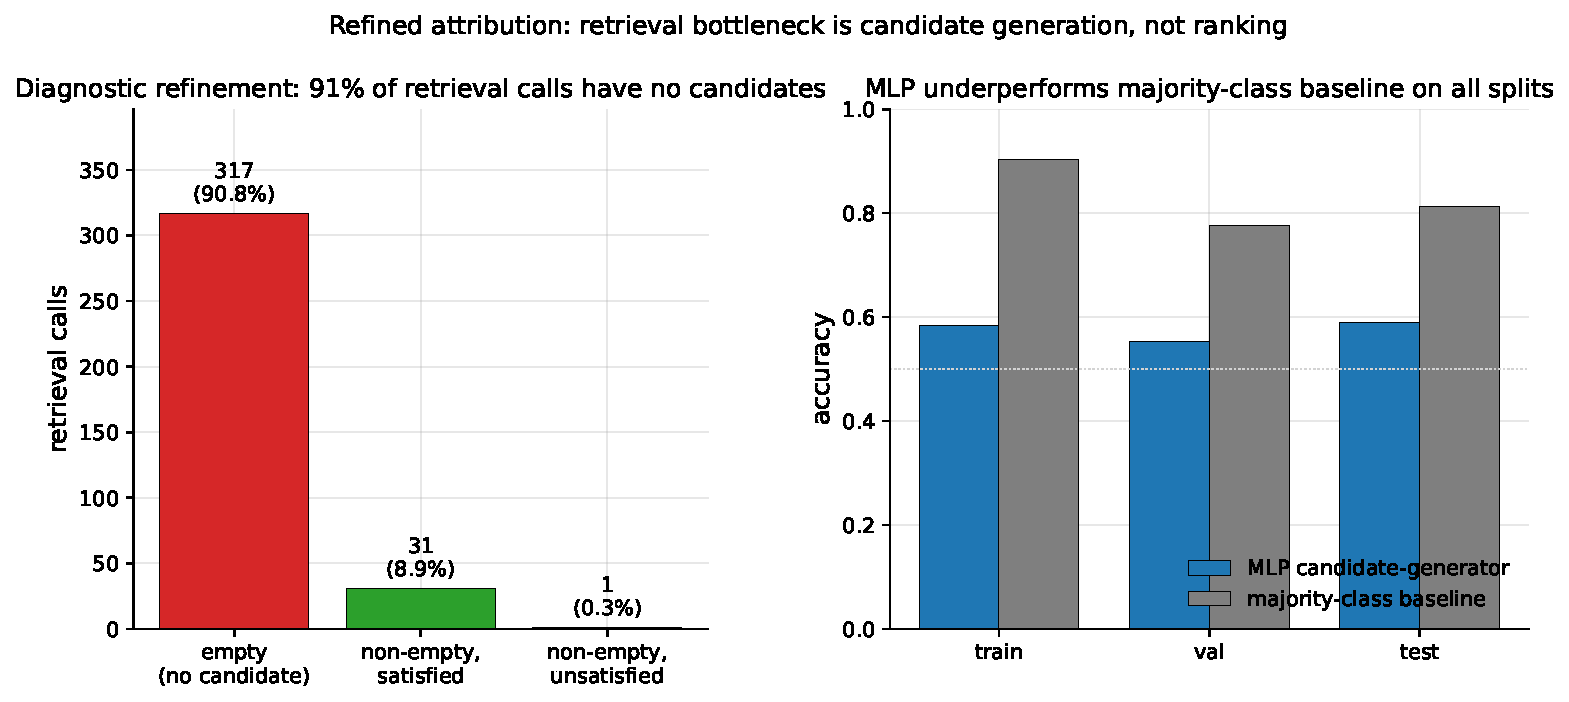
\includegraphics[width=0.95\linewidth]{figures/fig_refined_attribution.pdf}
\caption{Диагностика уточнённой атрибуции. \emph{Слева:} 349 вызовов извлечения, агрегированных по 10 сидам; 317 (90.8\%) вернули пустые множества кандидатов, 31 (8.9\%) вернул хотя бы одного удовлетворяющего кандидата, лишь 1 (0.3\%) вернул кандидатов, отранжированных, но неудовлетворяющих. Бутылочное горлышко --- генерация кандидатов, а не их ранжирование. \emph{Справа:} обученный MLP уступает мажоритарному бейзлайну на всех трёх сид-дизъюнктных разбиениях, подтверждая, что одних лишь мгновенных признаков состояния недостаточно для предсказания пригодности кандидата.}
\label{fig:refined-attribution}
\end{figure}

MLP уступает мажоритарному классу по точности на всех разбиениях и
достигает лишь умеренной precision при фиксированном recall. Мгновенных признаков
состояния недостаточно, чтобы предсказать пригодность кандидата ниже по потоку. Это
то самое негативное-но-информативное наблюдение, на которое ссылается \S\ref{sec:refined-attribution}:
атрибуция фреймворка «ограничено извлечением» уточняется до
«ограничено накоплением памяти», а не «ограничено ранжированием».

\subsection{Бейзлайн обученной коммуникации в стиле CommNet (\S\ref{sec:multi-agent-results})}

\textbf{Архитектура политики.} Наблюдение агента --- 4-мерный one-hot направления
$+$ локальное окно типов клеток $5\!\times\!5\!\times\!5$ (125) $+$ 2-мерная нормализованная
позиция $=$ 131. Энкодер с общими весами $131{\to}64{\to}64$ (ReLU), 16-мерная
проекция коммуникации, mean-pool по пирам (исключая себя), объединение $80{\to}64$ (ReLU),
голова актора $64\!\to\!4$ (TURN\_LEFT, TURN\_RIGHT, FORWARD, NOOP), голова критика
$64\!\to\!1$. Это архитектура обученной коммуникации в стиле CommNet~\citep{sukhbaatar2016commnet}.

\textbf{Обучение.} REINFORCE~\citep{williams1992simple} с ценностным бейзлайном; лосс $=\!-\,\mathrm{mean}(\log\pi(a)\cdot(R\!-\!V))\,+\,0.5\cdot\mathrm{MSE}(V,R)\,-\,0.01\cdot H[\pi]$; Adam $\text{lr}=3{\cdot}10^{-4}$, клиппинг градиента $1.0$. Шейпинг награды: $+1.0$ за первый успех на агента, $-0.01$ шаговая цена, $-0.1$ за контакт с опасностью. 2000 эпизодов с циклом по 200 сидам среды, настенное время $100$\,с на CPU. Оценка на отложенных 50 сидах среды 250--299.

\textbf{Кривая обучения.} Поэпизодный успех (окно последних 100) остаётся в
$[0.13, 0.23]$ на протяжении обучения; монотонного улучшения после $\sim\!200$
эпизодов нет. Политика сходится к локальному оптимуму, где один из трёх агентов
находит воду случайно.

\begin{figure}[h]
\centering
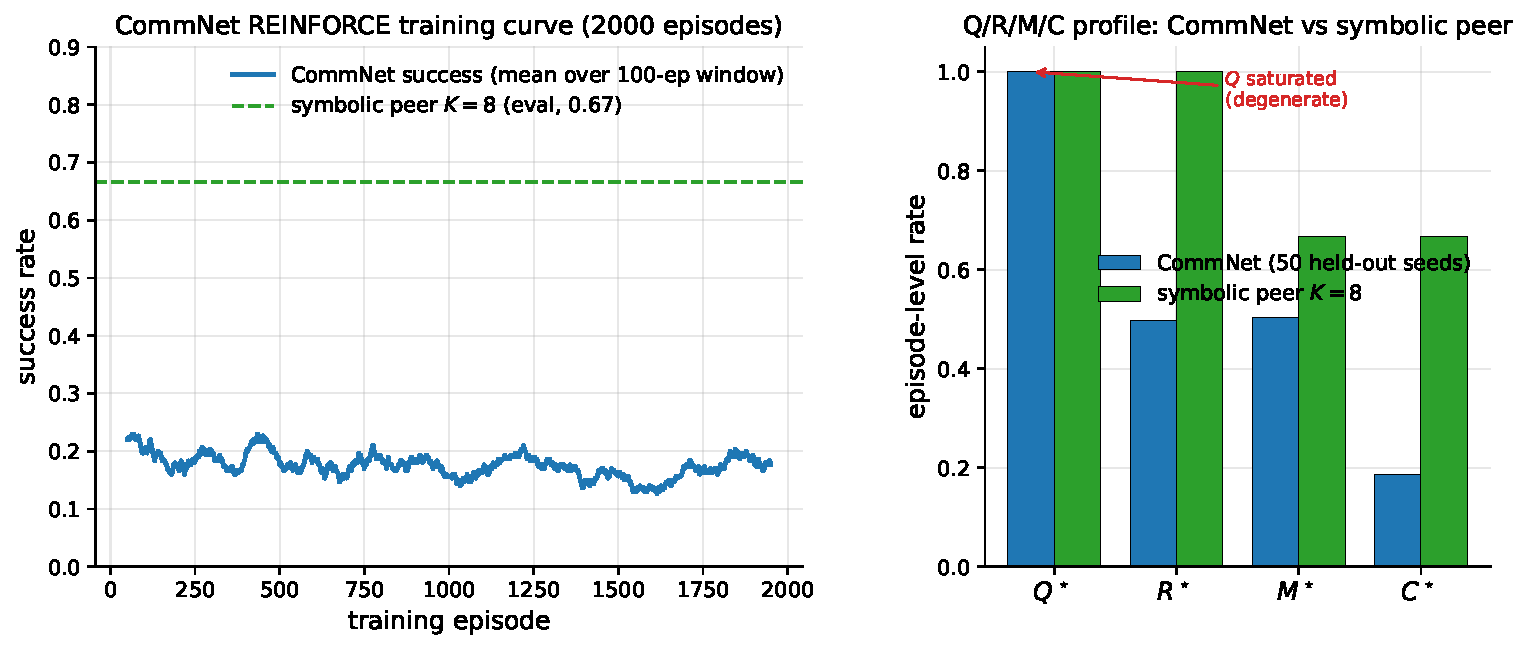
\includegraphics[width=0.95\linewidth]{figures/fig_commnet_baseline.pdf}
\caption{Диагностика бейзлайна обученной коммуникации. \emph{Слева:} кривая обучения CommNet (сглаженная доля успеха по окну в 100 эпизодов) на 2000 обучающих эпизодов; успех остаётся ниже 0.25 на всём протяжении. Пунктирная линия --- символьная пировая архитектура при $K\!=\!8$ на том же сценарии для сравнения. \emph{Справа:} профиль Q/R/M/C обученного CommNet на 50 отложенных сидах против символьного peer при $K\!=\!8$. $Q^\star$ насыщен на $1.0$ у CommNet (вырожден по построению); $R/M$ схлопываются вместе; только у символьной архитектуры условные частоты разделены.}
\label{fig:commnet}
\end{figure}

\textbf{Оценка Q/R/M/C (50 отложенных сидов, стохастическое сэмплирование действий).}

\begin{table}[h]
\centering
\small
\begin{tabular}{l c}
\toprule
Величина & Значение \\
\midrule
Частота $Q^\star$                              & \textbf{1.00} (насыщена) \\
Частота $R^\star$                              & 0.50 \\
Частота $M^\star$                              & 0.50 (схлопывается на $R$) \\
Частота $C^\star$                              & 0.19 \\
$P(R \mid Q)$                               & 0.50 \\
$P(M \mid R)$                               & 1.00 \\
$P(C \mid M)$                               & 0.42 \\
Доля успеха                                & 0.19 \\
Средние шаги                                  & 80 (бюджет исчерпан) \\
\bottomrule
\end{tabular}
\end{table}

Сравните с символьной пировой архитектурой при $K{=}8$: $P(M^\star|R^\star){=}0.69$, $P(C^\star|M^\star){=}0.87$, успех $\sim 0.65$.

\paragraph{Вариант PPO: структурная вырожденность верифицирована при конкурентоспособном успехе.}
Обученный PPO~\citep{schulman2017proximal} вариант той же архитектуры CommNet (клип $\epsilon{=}0.2$, обобщённая оценка преимущества~\citep{schulman2016gae} с $\lambda{=}0.95$, $\gamma{=}0.99$, 4 PPO-эпохи на роллаут, 64 роллаута на обновление, 200 обновлений, $\approx 96$ минут на одном ядре CPU; полная настройка в \texttt{experiments/commnet\_ppo\_baseline/train\_ppo\_commnet.py}) достигает успеха $0.667$ на 100 отложенных сидах --- конкурентоспособно с символьной пировой архитектурой при $K{=}8$ ($0.65$).

\begin{table}[h]
\centering
\small
\caption{REINFORCE против PPO CommNet против символьного peer ($K{=}8$) на сценарии дефицита ($N{=}3$, $T{=}2$, асимметричная, опасность $0.05$). PPO конкурентоспособен по доле успеха, но всё равно демонстрирует Q-насыщение и коллапс R/M --- диагностическое утверждение верифицировано, а не постулировано.}
\label{tab:ppo-commnet}
\begin{tabular}{l c c c}
\toprule
Метрика & CommNet REINFORCE & \textbf{CommNet PPO} & Симв. peer ($K{=}8$) \\
\midrule
Доля успеха                  & 0.19   & \textbf{0.667} & 0.65 \\
Частота $Q^\star$                & 1.00   & \textbf{1.00}  & 0.99 \\
Частота $R^\star$                & 0.50   & \textbf{0.997} & 0.69 \\
Частота $M^\star$                & 0.50   & \textbf{0.997} & 0.69 \\
$P(M^\star|R^\star)$          & 1.00   & \textbf{1.00}  & 0.69 \\
$P(C^\star|M^\star)$          & 0.42   & \textbf{0.67}  & 0.87 \\
R/M разделены?                & нет     & \textbf{нет}    & \textbf{да} \\
\bottomrule
\end{tabular}
\end{table}

Результат PPO превращает структурный аргумент из утверждения («бюджет обучения этого бы не изменил») в измерение: $Q^\star$ остаётся насыщенным на 1.00, $P(M^\star|R^\star)$ остаётся 1.00 (коллапс R/M) даже при конкурентоспособном успехе. Стадия Q вырождена по построению у любой политики, чей коммуникационный канал --- вещественный вектор с обученной линейной проекцией --- канал никогда не бывает информативно пустым, независимо от бюджета обучения, --- а без явного символьного интерфейса фиксации цели событие M не может отделиться от R. Только архитектуры с явным интерфейсом \emph{запроса/фиксации} (символьный стек из \S\ref{sec:archs}) обнажают постадийно разделимые события Q/R/M/C.

\section{Команды воспроизводимости}
\label{app:repro}

Подачу сопровождает анонимизированный публичный репозиторий. Артефакты основной статьи сгенерированы следующими скриптами; всюду предполагаются \texttt{PYTHONPATH=.} и виртуальное окружение Python 3 с \texttt{numpy}, \texttt{scipy}, \texttt{pandas}, \texttt{matplotlib}, \texttt{imageio}, \texttt{gymnasium} и \texttt{minigrid}.

\paragraph{Вычислительная инфраструктура.} Все эксперименты выполнялись на одной
потребительской машине: Apple Silicon (10 ядер CPU для свипов через
\texttt{ProcessPoolExecutor}), macOS (Darwin 25.4), Python 3.9.6.
Ключевые версии библиотек: \texttt{numpy} 1.x, \texttt{scipy},
\texttt{torch} (бейзлайн CommNet-PPO и VMAS), \texttt{vmas} 1.5.2,
\texttt{minigrid}/\texttt{gymnasium}. LLM-эксперименты используют локальные
модели через Ollama (\texttt{llama3.1:latest} 8B, \texttt{qwen3:4b}) при
температуре $0$ с детерминированным дисковым кэшированием ответов;
исследование внешних фреймворков дополнительно использует \texttt{openai} 2.44,
\texttt{langgraph} 0.6, \texttt{langchain-ollama} и
\texttt{pyautogen} 0.9 (классический AutoGen). GPU-кластер или платный API
не использовались; полный многоагентный блок воспроизводится за ${\approx}22$
минуты на 8 ядрах, а каждое LLM-исследование --- за минуты-часы локального
инференса.

\subsection*{Воспроизведение одной командой (многоагентный блок, $\approx 22$ минуты на 8 ядрах)}
\path{bash scripts/reproduce_paper.sh}

\subsection*{Чистая сюита Статьи 1}
\begin{itemize}[leftmargin=16pt]
\item smoke-сюита (все локальные не-LLM блоки): \path{python scripts/run_paper1_clean_experiments.py --mode smoke --skip_llm --out_dir tmp/paper1_clean_experiments_smoke}
\item полная локальная сюита (одноагентный, оракульный, многоагентный, CommNet, переносимость/шум): \path{python scripts/run_paper1_clean_experiments.py --mode full --skip_llm --workers 8 --out_dir tmp/paper1_clean_experiments_full}
\item свип бюджета шагов LLM TextNav (требует локальный Ollama), запуск один раз на бюджет $K'\in\{6,12,25\}$: \path{python -m experiments.llm_collective.run_model_sweep --models qwen3:4b llama3.1:latest --episodes 8 --step_limit <K'> --out_dir tmp/llm_steplimit_<K'>}
\end{itemize}

\subsection*{Один агент (\S\ref{sec:validation}--\S\ref{sec:oracle})}
\begin{itemize}[leftmargin=16pt]
\item статейный бенчмарк и сюита обученных бейзлайнов: \path{scripts/benchmark_symbolic_memory_article.py}
\item статейный анализ и генерация рисунков: \path{scripts/analyze_symbolic_memory_article.py}
\item синтетическая проверка корректности факторизации: \path{scripts/validate_qrmc_factorization.py}
\item бенчмарк оракульных постадийных интервенций: \path{scripts/benchmark_oracle_stage_interventions.py}
\item бенчмарк переноса на BabyAI: \path{scripts/compare_semnav_babyai.py}
\end{itemize}

\subsection*{Много агентов (\S\ref{sec:multi-agent-results})}
\begin{itemize}[leftmargin=16pt]
\item Базовый батч --- peer при $K\in\{1,2,4,8,16\}$ \emph{и} три бескаденционные архитектуры (независимая, общая шина, центральный агрегатор), 40 сидов ($25{,}920$ прогонов $=16{,}200$ peer $+\,9{,}720$ бескаденционных), $\approx 18$ мин:
\path{python experiments/big_experiment/exp_cadence_phase.py --mode full --workers 8 --out_dir tmp/big_experiment_qrmc_40}
\item Батч расширенных каденций --- только peer при $K\in\{32,48,64\}$ ($9{,}720$ прогонов), $\approx 4$ мин:
\path{python experiments/big_experiment/exp_extra_K.py --workers 8 --out_dir tmp/big_experiment_extraK}
\item[] \emph{Замечание.} Эти два батча разбивают итог $35{,}640$ по \emph{диапазону каденций}; поархитектурное разбиение из Приложения~\ref{app:design} ($25{,}920$ peer по всем восьми каденциям против $9{,}720$ бескаденционных) переиспользует те же два итога для \emph{разных} подмножеств (совпадение: $3$ расширенные каденции $\times\,3{,}240 = 3$ бескаденционные архитектуры $\times\,3{,}240$). Объединённый лог --- \path{tmp/paper1_clean_experiments_full/multiagent_cadence_full/runs.csv}.
\item Постадийный анализ Q/R/M/C и бутстреп-ДИ:
\path{python experiments/big_experiment/analyze_qrmc.py --runs_csv tmp/big_experiment_qrmc_40/runs.csv --out_dir tmp/big_experiment_qrmc_40}
\item Многоагентные оракульные интервенции:
\path{python experiments/big_experiment/exp_oracle_interventions.py --workers 8 --out_dir tmp/big_experiment_oracle}
\item Smoke-тесты фаз 1--4:
\path{python scripts/run_all_smokes.py --out_dir tmp/all_smokes}
\item Обученный PPO бейзлайн CommNet (Таблица~\ref{tab:ppo-commnet}, $\approx 96$ мин на одном ядре CPU):
\path{python -m experiments.commnet_ppo_baseline.train_ppo_commnet --total_updates 200 --rollouts_per_update 64}
\item Оценка Q/R/M/C политики PPO на 100 отложенных сидах:
\path{python experiments/commnet_baseline/eval_with_qrmc.py --policy_path experiments/commnet_ppo_baseline/ppo_policy.pt --out_dir experiments/commnet_ppo_baseline --n_episodes 100}
\item Свип переносимости на субстрате MiniGrid (\S\ref{sec:limitations}, 100 прогонов, $\approx 2$ мин):
\path{python -m experiments.minigrid_multiagent_wrapper.run_portability_sweep --out_dir tmp/minigrid_portability}
\end{itemize}

\section{Замечание об ассетах и лицензиях}
\label{app:assets}

Эксперименты используют MiniGrid~\citep{MinigridMiniworld23} и BabyAI~\citep{chevalier2018babyai}, оба выпущены под лицензией MIT. Локально реализованные бейзлайны и скрипты запуска бенчмарков, введённые в этой статье, будут выпущены под лицензией MIT в составе пакета артефактов camera-ready.

\clearpage
\FloatBarrier
\input{checklist.tex}

\end{document}
